% !TEX program = xelatex
% Tiny210 / S5PV210 ARM32 专题书稿
\documentclass[UTF8,zihao=-4,fontset=none,oneside]{ctexbook}

\usepackage[a4paper,top=24mm,bottom=24mm,left=22mm,right=22mm,headheight=16pt]{geometry}
\usepackage{xcolor}
\usepackage{booktabs,longtable,tabularx,array}
\usepackage{listings}
\usepackage{fancyvrb}
\usepackage{graphicx}
\usepackage{tikz}
\usepackage{float}
\usepackage{caption}
\usepackage{enumitem}
\usepackage{fancyhdr}
\usepackage{hyperref}
\usetikzlibrary{arrows.meta,positioning,shapes.geometric,fit,calc,matrix}

% 优先使用开发主机上的中文字体；在没有这些字体的 TeX Live 环境中回退 Fandol。
\IfFontExistsTF{Songti SC}{
  \setCJKmainfont[AutoFakeBold=2]{Songti SC}
  \setCJKsansfont[AutoFakeBold=2]{Hiragino Sans GB}
  \setCJKmonofont[AutoFakeBold=2]{Hiragino Sans GB}
}{
  \setCJKmainfont[AutoFakeBold=2]{FandolSong-Regular}
  \setCJKsansfont[AutoFakeBold=2]{FandolHei-Regular}
  \setCJKmonofont[AutoFakeBold=2]{FandolFang-Regular}
}
\IfFontExistsTF{Menlo}{\setmonofont{Menlo}}{}

\definecolor{tinyblue}{RGB}{17,91,122}
\definecolor{tinycyan}{RGB}{23,139,166}
\definecolor{tinyred}{RGB}{155,45,55}
\definecolor{tinygreen}{RGB}{28,113,83}
\definecolor{codebg}{RGB}{247,249,250}
\definecolor{codecomment}{RGB}{104,116,126}

\hypersetup{
  unicode=true,
  colorlinks=true,
  linkcolor=tinyblue,
  urlcolor=tinycyan,
  citecolor=tinyred,
  bookmarksnumbered=true,
  bookmarksopen=true,
  pdftitle={从裸机到系统：Tiny210 / ARMv7-A},
  pdfauthor={Jiming Kang}
}

\pagestyle{fancy}
\fancyhf{}
\fancyhead[L]{Tiny210 / ARMv7-A}
\fancyhead[R]{\leftmark}
\fancyfoot[C]{\thepage}
\renewcommand{\headrulewidth}{0.4pt}

\setcounter{tocdepth}{2}
\setcounter{secnumdepth}{3}
\setlength{\parindent}{2em}
\setlength{\parskip}{0.25em}
\setlength{\emergencystretch}{3em}
\setlength{\LTleft}{0pt}
\setlength{\LTright}{0pt}
\setlength{\tabcolsep}{4pt}
\setlist{nosep,leftmargin=2.2em}

\lstdefinelanguage{armasm}{
  sensitive=false,
  morekeywords={mov,movw,movt,ldr,ldrb,str,strb,ldm,stm,push,pop,add,sub,
    and,orr,bic,eor,lsl,lsr,asr,cmp,tst,b,bl,bx,blx,svc,mrc,mcr,isb,dsb,dmb,
    cpsid,cpsie,wfi,nop},
  morecomment=[l]{@},morecomment=[l]{//},morecomment=[s]{/*}{*/},morestring=[b]"
}
\lstdefinelanguage{mermaid}{
  sensitive=true,
  morekeywords={flowchart,graph,sequenceDiagram,stateDiagram-v2,participant,as,
    Note,over,rect,end,subgraph,style,classDef}
}
\lstset{
  basicstyle=\ttfamily\small,
  keywordstyle=\color{tinyred}\bfseries,
  commentstyle=\color{codecomment},
  stringstyle=\color{tinygreen},
  backgroundcolor=\color{codebg},
  frame=single,
  rulecolor=\color{tinyblue!35},
  framerule=0.35pt,
  breaklines=true,
  columns=fullflexible,
  keepspaces=true,
  showstringspaces=false,
  tabsize=2,
  xleftmargin=3pt,
  xrightmargin=3pt,
  aboveskip=6pt,
  belowskip=6pt
}

\tikzset{
  box/.style={draw=tinyblue!75!black,rounded corners=2pt,fill=tinyblue!7,
    align=center,minimum height=8mm,inner sep=4pt,font=\small},
  hbox/.style={box,fill=tinycyan!18},
  gbox/.style={box,draw=gray!65,fill=gray!8},
  arr/.style={-{Stealth[length=2.2mm]},thick,draw=tinyblue!80!black},
  darr/.style={arr,dashed},
  lab/.style={font=\footnotesize,text=gray!70!black}
}

% Pandoc 生成章节时使用的兼容宏。
\providecommand{\tightlist}{\setlength{\itemsep}{0pt}\setlength{\parskip}{0pt}}
\providecommand{\passthrough}[1]{#1}
\providecommand{\pandocbounded}[1]{#1}
\newcounter{none}

\title{从裸机到系统\\[4pt]\Large Tiny210 / S5PV210 ARMv7-A 实现}
\author{Jiming Kang\\\small xv6-aarch64 项目}
\date{2026 年 11 月\\\small 版本 0.1}

\begin{document}

\frontmatter
\maketitle

\chapter*{关于本书}
\addcontentsline{toc}{chapter}{关于本书}
本书面向 FriendlyARM Tiny210 开发者，以 Samsung S5PV210、ARMv7-A 和当前
\texttt{tiny210} 分支为唯一对象。它不把 Raspberry Pi 3 的 AArch64、GIC、DWC2
板载拓扑或 BCM43430 路径混入正文，而是沿 Tiny210 的真实依赖链讲解：iROM/BL1、
ARM32 异常向量和 VIC、PWM 时钟、FIMD、SDHCI、EHCI、MT7601U、VFS 与 xv6fs。

正文由 \texttt{doc/readme/tiny210} 下的专题 Markdown 整理而来；代码和寄存器值
以仓库当前实现为准。QEMU 使用的 Cubieboard 只是 ARM32 通用逻辑替身，不能代替
Tiny210 实板验证。

\tableofcontents

\mainmatter
\chapter{Tiny210
开发者指南}\label{tiny210-ux5f00ux53d1ux8005ux6307ux5357}

本文档集面向在 FriendlyARM Tiny210（Samsung S5PV210、ARM
Cortex-A8）上开发 xv6 的人员。默认目标是 Tiny210；同一端口也可通过
\passthrough{\lstinline!S5PV210\_BOARD=x210!} 构建九鼎 X210，但两块板的
DRAM、串口和机器号不同。

\begin{quote}
当前状态：S5PV210 实板路径与 QEMU 替身路径共用 ARM32 内核框架。QEMU 使用
\passthrough{\lstinline!cubieboard!}（Allwinner A10）验证通用
ARM32、initcall、platform bus、 进程和文件系统逻辑，并不能验证 S5PV210
的 VIC、PWM、FIMD、DDR 时序和引脚。 修改寄存器驱动后仍需 Tiny210
实板验证。
\end{quote}

\section{阅读顺序}\label{ux9605ux8bfbux987aux5e8f}

\begin{enumerate}
\def\labelenumi{\arabic{enumi}.}
\tightlist
\item
  \href{boot.md}{启动与内存初始化}：从 iROM/BL1 到第一个用户进程。
\item
  \href{interrupts.md}{异常、中断与系统时钟}：异常向量、VIC、PWM Timer 4
  和调度 tick。
\item
  \href{lcd.md}{LCD/FIMD}：面板时序、FIMD DMA scanout、framebuffer 与
  fbcon。
\item
  \href{wifi.md}{MT7601U Wi-Fi}：EHCI 枚举、固件、SoftMAC、WPA2、NAPI 和
  DHCP。
\item
  \href{filesystem.md}{文件系统}：内嵌 xv6fs、bcache、redo log 和
  \passthrough{\lstinline!/init!}。
\item
  \href{drivers.md}{驱动模型与板载按键}：platform
  device/driver、resource、initcall、 K1-\/-K8 输入子系统和
  \passthrough{\lstinline!event0!}。
\item
  \href{bringup-notes.md}{上板调试记录}：串口乱码、EHCI 欠载、iROM 读第
  0 扇区卡死、BL1 入口偏移与对齐错误等问题的现象、原因和解决办法。
\end{enumerate}

\section{代码地图}\label{ux4ee3ux7801ux5730ux56fe}

\begin{lstlisting}
ports/tiny210/
|-- Makefile             Tiny210/X210 构建入口
|-- mktiny210.py         BL1、uImage、整卡镜像生成与校验
`-- test_shell.py        QEMU shell 回归测试

kernel/arch/arm/
|-- vectors.S            ARMv7 异常向量和 trapframe 保存/恢复
|-- irq.c                request_irq() 与通用 IRQ 分派
|-- time.c               clocksource、ticks、调度 tick
|-- vm.c                 ARMv7 short-descriptor 页表和 MMU
`-- initcall.c           按 level/order 执行内置驱动

kernel/arch/arm/mach-s5pv210/
|-- bl1/                 自带第一阶段引导程序
|-- entry.S              内核物理入口、各模式栈、VBAR
|-- setup.c              x210_main() 和板级启动
|-- devices.c            S5PV210 platform device/resource 表
|-- board.h              Tiny210/X210 板级差异
|-- memlayout.h          DRAM、用户空间和 framebuffer 布局
`-- atag.c               ARM Linux ATAG 解析

kernel/drivers/
|-- clk/clk-s5pv210.c
|-- irqchip/irq-vic.c
|-- clocksource/samsung_pwm_timer.c
|-- tty/serial/samsung.c
|-- watchdog/s3c2410_wdt.c
|-- video/fbdev/s3c-fb.c
|-- video/fbdev/fbcon.c
|-- input/keyboard/s5pv210-keys.c
|-- usb/host/ehci-hcd.c
|-- usb/core/usb.c
|-- net/wireless/mt7601u.c
`-- block/ramdisk_embed.c
\end{lstlisting}

\section{快速构建}\label{ux5febux901fux6784ux5efa}

在仓库根目录执行：

\begin{lstlisting}[language=sh]
make tiny210
\end{lstlisting}

生成整卡镜像并写入已挂载的 SD 卡（BL1 到第 1 扇区、uImage 到第 49
扇区，MBR 不动，写后读回校验）：

\begin{lstlisting}[language=sh]
make tiny210-sdimg
\end{lstlisting}

等价的显式 Tiny210 构建是：

\begin{lstlisting}[language=sh]
make -f ports/tiny210/Makefile \
  S5PV210_BOARD=tiny210 \
  S5PV210_LCD=s70
\end{lstlisting}

主要产物位于 \passthrough{\lstinline!build/tiny210/!}：

{\def\LTcaptype{none} % do not increment counter
\begin{longtable}[]{@{}p{0.34\linewidth}p{0.60\linewidth}@{}}
\toprule\noalign{}
产物 & 作用 \\
\midrule\noalign{}
\endhead
\bottomrule\noalign{}
\endlastfoot
\passthrough{\lstinline!tiny210-bl1.bin!} & 16 KiB、带 iROM 头的
BL1，写入 SD 扇区 1 \\
\passthrough{\lstinline!xv6-tiny210.uImage!} & legacy uImage；写在
第 49 扇区，是 BL1 唯一的启动内核 \\
\passthrough{\lstinline!tiny210-sd.img!} & BL1@1 与 uImage@49
已放到固定扇区的整卡原始镜像 \\
\passthrough{\lstinline!kernel.elf!} /
\passthrough{\lstinline!kernel.map!} & 带符号调试文件和链接映射 \\
\passthrough{\lstinline!fs.img!} & 4 MiB xv6fs；构建时会被嵌入内核
\passthrough{\lstinline!.ramdisk!} \\
\end{longtable}
}

构建与 QEMU 回归测试：

\begin{lstlisting}[language=sh]
make tiny210-check
make tiny210-qemu
\end{lstlisting}

更换 \passthrough{\lstinline!S5PV210\_BOARD!}、LCD 型号或
\passthrough{\lstinline!BUILD!} 配置时先清理，避免复用旧目标文件：

\begin{lstlisting}[language=sh]
make tiny210-clean
\end{lstlisting}

\section{默认硬件参数}\label{ux9ed8ux8ba4ux786cux4ef6ux53c2ux6570}

{\def\LTcaptype{none} % do not increment counter
\begin{longtable}[]{@{}p{0.34\linewidth}p{0.60\linewidth}@{}}
\toprule\noalign{}
项目 & Tiny210 默认值 \\
\midrule\noalign{}
\endhead
\bottomrule\noalign{}
\endlastfoot
CPU & Samsung S5PV210 / Cortex-A8，单核 \\
DRAM & 512 MiB，物理起始 \passthrough{\lstinline!0x20000000!} \\
内核入口 & \passthrough{\lstinline!0x20008000!} \\
ATAG & \passthrough{\lstinline!0x20000100!} \\
机器号 & 3466（MINI210） \\
串口 & UART0 / COM0，115200 8N1 \\
IRQ 控制器 & 4 个 PL192 VIC，IRQ 0..127 \\
系统 tick & PWM Timer 4，IRQ 25 \\
LCD & S70 800×480，XRGB8888（可编译选择其他面板） \\
根文件系统 & 优先 FAT32 中的
\passthrough{\lstinline!FS.IMG!}，找不到时回退内嵌 xv6fs RAM 镜像 \\
\end{longtable}
}

\section{启动全景}\label{ux542fux52a8ux5168ux666f}

\begin{figure}[htbp]
\centering
\resizebox{\linewidth}{!}{\begin{tikzpicture}[node distance=5mm]
  \node[hbox] (rom) {S5PV210 iROM\\BL0};
  \node[box,right=of rom] (bl1) {BL1 / iRAM\\时钟、UART、DDR};
  \node[box,right=of bl1] (mbr) {LBA 0 / MBR\\定位 FAT32};
  \node[box,right=of mbr] (img) {根目录文件\\加载 uImage};
  \node[box,right=of img] (entry) {\texttt{\_entry}\\ARM32 环境};
  \node[box,right=of entry] (main) {\texttt{x210\_main()}\\MMU、设备、进程};
  \node[hbox,right=of main] (user) {\texttt{/init}\\\texttt{/bin/sh}};
  \draw[arr] (rom)--(bl1); \draw[arr] (bl1)--(mbr); \draw[arr] (mbr)--(img); \draw[arr] (img)--(entry);
  \draw[arr] (entry)--(main); \draw[arr] (main)--(user);
\end{tikzpicture}}
\caption{Tiny210 从上电到第一个用户 shell 的主路径}
\label{fig:tiny-overview}
\end{figure}


\section{当前实现边界}\label{ux5f53ux524dux5b9eux73b0ux8fb9ux754c}

\begin{itemize}
\tightlist
\item
  内核使用 ARMv7 short-descriptor 页表和恒等映射；cache 在当前 bring-up
  中关闭。
\item
  只启用单 CPU；没有 SMP/GIC 路径。
\item
  UART 输入不是 UART IRQ 驱动，而是每次 PWM tick 调用
  \passthrough{\lstinline!uartintr()!} 轮询。
\item
  K1-\/-K8 使用 GPH2/GPH3 外部中断和 20 ms 延迟消抖，通过
  \passthrough{\lstinline!/dev/input/event0!} 输出 Linux 风格
  \passthrough{\lstinline!EV\_KEY!}/\passthrough{\lstinline!EV\_SYN!}
  事件。
\item
  LCD 只有 FIMD Window 0、单 framebuffer、32 bpp；没有 VSync
  IRQ、双缓冲或用户态 mmap。
\item
  实板构建已包含 SDHCI、FAT32、VFS 和 ext2；QEMU 构建仍使用内嵌 RAM
  镜像。
\item
  USB-A/EHCI 和 MT7601U 已接入，但 EHCI 尚无运行时热插拔，QEMU
  也无法验证。
\item
  \passthrough{\lstinline!DEVICE\_MAX!} 和字符设备表等仍是静态上限，不是
  Linux 的动态对象模型。
\end{itemize}

\section{实板调试入口}\label{ux5b9eux677fux8c03ux8bd5ux5165ux53e3}

\begin{itemize}
\tightlist
\item
  串口先看 BL1 是否打印；完全无输出时优先检查启动拨码、COM0、115200
  8N1。
\item
  BL1
  可单独构建串口测试：\passthrough{\lstinline!make -f ports/tiny210/Makefile uarttest!}。
\item
  内核加载前失败依次看
  \passthrough{\lstinline!tiny210-bl1.bin!}、第 49 扇区的
  \passthrough{\lstinline!xv6-tiny210.uImage!} 和 uImage CRC；
  根文件系统的 FAT32/raw 探测错误属于内核侧；内核入口失败看
  \passthrough{\lstinline!\_entry!}。
\item
  进入内核后按 \passthrough{\lstinline!initcall:!} 日志判断失败属于
  clock、VIC、timer、serial 还是 LCD probe。
\item
  LCD 无显示但串口正常时，先选择正确
  \passthrough{\lstinline!S5PV210\_LCD!}，再核对 RGB 排线、供电和背光。
\item
  完整烧录步骤与风险提示见
  \href{../../../ports/tiny210/README.md}{ports/tiny210/README.md}。
\end{itemize}

\chapter{Tiny210
启动与内存初始化}\label{tiny210-ux542fux52a8ux4e0eux5185ux5b58ux521dux59cbux5316}

\section{SD 启动布局}\label{sd-ux542fux52a8ux5e03ux5c40}

Tiny210 不依赖 U-Boot。S5PV210 iROM（BL0）从 SD 卡固定位置加载本仓库的
BL1； BL1 初始化 SDHCI 后读取 MBR，在第一个 FAT32
分区的根目录中查找并加载 \passthrough{\lstinline!xv6\_tiny210.img!}：

{\def\LTcaptype{none} % do not increment counter
\begin{longtable}[]{@{}p{0.18\linewidth}p{0.26\linewidth}p{0.50\linewidth}@{}}
\toprule\noalign{}
SD 扇区 & 内容 & 运行/加载位置 \\
\midrule\noalign{}
\endhead
\bottomrule\noalign{}
\endlastfoot
0 & MBR，制作镜像时保留 & 不执行 \\
1..32 & 16 KiB \passthrough{\lstinline!tiny210-bl1.bin!} & iRAM
\passthrough{\lstinline!0xD0020000!}，代码入口
\passthrough{\lstinline!0xD0020010!} \\
33..48 & 保留 & --- \\
49.. & 原始 uImage 救援副本（可选） & FAT32 文件不可用时才读取 \\
MBR 指定的 FAT32 分区 & 根目录
\passthrough{\lstinline!xv6\_tiny210.img!} & 主启动内核；先放到
DRAM+\passthrough{\lstinline!0x7fc0!}，uImage payload 位于
DRAM+\passthrough{\lstinline!0x8000!} \\
\end{longtable}
}

BL1 的前 16 字节是 iROM 所需的大小、保留字段和字节校验和。链接脚本
\href{../../../kernel/arch/arm/mach-s5pv210/bl1/bl1.ld}{\passthrough{\lstinline!bl1/bl1.ld!}}
强制代码不超过 \passthrough{\lstinline!16 KiB - 16 B!}。

\section{BL0 → BL1 → 内核}\label{bl0--bl1--ux5185ux6838}

\begin{figure}[htbp]
\centering
\resizebox{\linewidth}{!}{%
\begin{tikzpicture}[node distance=7mm]
  \node[hbox] (rom) {iROM / BL0\\读扇区 1--32};
  \node[box,below=of rom] (bl1) {BL1 @ \texttt{0xD0020010}\\校验头、PS\_HOLD、PLL、UART};
  \node[box,below=of bl1] (ddr) {初始化 DMC0 DDR2\\容量和读写测试};
  \node[box,below=of ddr] (sd) {初始化启动通道的 SDHCI PIO\\读取 LBA 0};
  \node[box,below=of sd] (mbr) {校验 MBR \texttt{0x55AA}\\选择首个 \texttt{0x0b/0x0c} 分区};
  \node[box,below left=7mm and 10mm of mbr] (fat) {解析 FAT32 BPB、FAT、根目录\\读取 \texttt{xv6\_tiny210.img}};
  \node[gbox,below right=7mm and 10mm of mbr] (raw) {MBR、FAT32 或文件失败\\扇区 49 救援 uImage};
  \node[box,below=20mm of mbr] (atag) {加载到 \texttt{0x20007fc0} 并校验 uImage\\生成 ATAG：\texttt{r0=0, r1=3466, r2=0x20000100}};
  \node[hbox,below=of atag] (kernel) {跳到 \texttt{0x20008000}\\内核 \texttt{\_entry}};
  \draw[arr] (rom)--(bl1); \draw[arr] (bl1)--(ddr); \draw[arr] (ddr)--(sd); \draw[arr] (sd)--(mbr);
  \draw[arr] (mbr)--(fat); \draw[arr] (mbr)--(raw);
  \draw[arr] (fat)--(atag); \draw[arr] (raw)--(atag); \draw[arr] (atag)--(kernel);
\end{tikzpicture}
}
\caption{MBR/FAT32 内核加载主路径与固定扇区救援回退}
\label{fig:tiny-boot-chain}
\end{figure}


BL1 入口在
\href{../../../kernel/arch/arm/mach-s5pv210/bl1/start.S}{\passthrough{\lstinline!bl1/start.S!}}，
硬件初始化和加载决策在
\href{../../../kernel/arch/arm/mach-s5pv210/bl1/bl1.c}{\passthrough{\lstinline!bl1/bl1.c!}}，
FAT32 只读实现位于
\href{../../../kernel/arch/arm/mach-s5pv210/bl1/bl1fat.c}{\passthrough{\lstinline!bl1/bl1fat.c!}}。
由于实板 iROM 的 \passthrough{\lstinline!CopySDMMCtoMem!} 读取 LBA 0
会卡住，主路径复用
\href{../../../kernel/drivers/mmc/host/sdcore.c}{\passthrough{\lstinline!sdcore.c!}}
的小型 SDHCI PIO 核心读取 MBR、FAT 和文件数据；iROM 复制服务只保留给扇区
49 的救援回退。

BL1 的 FAT32 加载顺序为：

\begin{lstlisting}
LBA 0
  -> 校验 0x55AA
  -> 扫描 4 个 MBR partition entry
  -> 选择第一个 type=0x0b/0x0c 的 FAT32 分区
  -> 读取 VBR/BPB，计算 fat_lba、data_lba、root_cluster
  -> 遍历根目录 cluster chain
  -> 匹配 xv6_tiny210.img 的 VFAT 长文件名或 8.3 别名
  -> 沿 FAT cluster chain 把文件读到 DRAM+0x7fc0
  -> 校验 uImage header、load/entry、文件长度和 data CRC
\end{lstlisting}

只有 MBR/FAT32 无效或根目录找不到内核文件时，BL1 才读取固定扇区 49
的救援 uImage。这样日常升级只需替换 FAT32 文件，不必重新写内核原始扇区。

交接遵循 ARM Linux 传统启动约定：

\begin{lstlisting}
r0 = 0
r1 = 3466 (MINI210 machine ID)
r2 = 0x20000100 (ATAG list)
CPU = SVC mode，IRQ/FIQ 屏蔽，MMU/D-cache 关闭
\end{lstlisting}

\section{\texorpdfstring{\texttt{\_entry}
做什么}{\_entry 做什么}}\label{_entry-ux505aux4ec0ux4e48}

内核入口是
\href{../../../kernel/arch/arm/mach-s5pv210/entry.S}{\passthrough{\lstinline!entry.S!}}
中的 \passthrough{\lstinline!\_entry!}：

\begin{enumerate}
\def\labelenumi{\arabic{enumi}.}
\tightlist
\item
  检查实际运行地址是否等于链接地址。
\item
  拒绝 USR mode 或仍开启 MMU 的错误启动方式。
\item
  关闭 I-cache/D-cache，设置低向量/非 VIC vectored 模式。
\item
  分别设置 IRQ、Abort、Undefined 和 SVC 各模式的栈。
\item
  清空 \passthrough{\lstinline!.bss!}。
\item
  把 VBAR 指向
  \href{../../../kernel/arch/arm/vectors.S}{\passthrough{\lstinline!vectors.S!}}
  的 \passthrough{\lstinline!vectors!}。
\item
  保留 \passthrough{\lstinline!r0/r1/r2!} 并调用
  \passthrough{\lstinline!x210\_main()!}。
\end{enumerate}

链接地址由
\href{../../../kernel/arch/arm/mach-s5pv210/kernel.ld}{\passthrough{\lstinline!kernel.ld!}}
的 \passthrough{\lstinline!KERNEL\_LOAD!} 决定；Tiny210 默认为
\passthrough{\lstinline!0x20008000!}。代码、只读数据、initcall 表、
数据和内嵌 ramdisk 都位于镜像中，\passthrough{\lstinline!.bss!}
不占镜像文件空间。

\section{\texorpdfstring{\texttt{x210\_main()}
内核初始化顺序}{x210\_main() 内核初始化顺序}}\label{x210_main-ux5185ux6838ux521dux59cbux5316ux987aux5e8f}

\href{../../../kernel/arch/arm/mach-s5pv210/setup.c}{\passthrough{\lstinline!setup.c!}}
的 \passthrough{\lstinline!x210\_main()!} 是板级 启动主线：

\begin{lstlisting}
uartinit()                         早期串口可立即打印
read_bootparams(r2)               解析 ATAG 或 DTB
kvminit(); kvminithart()          建立并启用内核页表
kinit1()                          初始化物理页分配器
device_init()                     注册 platform bus
consoleinit(); ttyinit()          控制台与 tty 字符设备
printfinit()
arm32_time_init()                 初始化 tickslock
s5pv210_register_devices()        登记板级控制器资源
do_initcalls()                    驱动注册、匹配并 probe
procinit(); binit(); iinit(); fileinit()
userinit()                        创建第一个用户进程
scheduler()                       不再返回
\end{lstlisting}

文件系统初始化没有直接放在 \passthrough{\lstinline!x210\_main()!}
中，因为日志恢复和 buffer lock 可能睡眠。 第一个普通进程第一次执行
\passthrough{\lstinline!forkret()!} 时调用
\passthrough{\lstinline!fsinit(ROOTDEV)!}，然后才返回用户态。

\section{内存布局与 MMU}\label{ux5185ux5b58ux5e03ux5c40ux4e0e-mmu}

Tiny210 DMC0 的物理 DRAM 从 \passthrough{\lstinline!0x20000000!}
开始。当前端口只把前 128 MiB 交给 页分配器，并在紧随其后的区域保留 2 MiB
framebuffer：

\begin{lstlisting}
0x20000000  +-------------------------------+
            | ATAG @ +0x100                 |
            | kernel @ +0x8000              |
            | text/rodata/data/ramdisk/bss  |
            | kalloc 可用页                  |
0x28000000  +-------------------------------+  DRAM + 128 MiB
            | LCD framebuffer (2 MiB)       |
0x28200000  +-------------------------------+
            | 当前内核未交给页分配器的 DRAM |
0x40000000  +-------------------------------+  512 MiB 顶端
\end{lstlisting}

\href{../../../kernel/arch/arm/vm.c}{\passthrough{\lstinline!vm.c!}}
使用 ARMv7 short-descriptor：

\begin{itemize}
\tightlist
\item
  内核 DRAM 采用 1 MiB section 恒等映射，VA 等于 PA。
\item
  \passthrough{\lstinline!devices.c!} 中每个
  \passthrough{\lstinline!IORESOURCE\_MEM!} 也建立恒等映射。
\item
  控制器寄存器映射为 privileged、strongly ordered、XN。
\item
  framebuffer 映射为 privileged、Normal non-cacheable、XN。
\item
  用户地址范围为 \passthrough{\lstinline![0, 0x20000000)!}，低于 Tiny210
  DRAM 起始地址。
\item
  当前 bring-up 中 CPU cache
  保持关闭，便于先保证设备一致性，但性能较低。
\end{itemize}

\section{第一个用户进程}\label{ux7b2cux4e00ux4e2aux7528ux6237ux8fdbux7a0b}

\passthrough{\lstinline!userinit()!} 的一页用户地址空间里放入
\href{../../../kernel/arch/arm/initcode.S}{\passthrough{\lstinline!initcode.S!}}：

\begin{lstlisting}
userinit()
  -> uvminit(..., initcode)
  -> PC=0, SP=4096, CPSR=user mode
  -> RUNNABLE
  -> scheduler()
  -> forkret()
       -> 首次 fsinit(ROOTDEV)
       -> usertrapret()
  -> initcode: exec("/init")
  -> /init: 创建 /dev 节点、连接 ttyS0、fork/exec /bin/sh
\end{lstlisting}

Tiny210 构建实际使用
\href{../../../kernel/arch/arm/init.c}{\passthrough{\lstinline!kernel/arch/arm/init.c!}}，
而不是仓库根用户集合中的 \passthrough{\lstinline!user/init.c!}。

\section{启动故障定位}\label{ux542fux52a8ux6545ux969cux5b9aux4f4d}

{\def\LTcaptype{none} % do not increment counter
\begin{longtable}[]{@{}p{0.34\linewidth}p{0.60\linewidth}@{}}
\toprule\noalign{}
最后可见信息 & 优先检查 \\
\midrule\noalign{}
\endhead
\bottomrule\noalign{}
\endlastfoot
完全无串口 & SD 启动拨码、BL1 扇区、UART0/COM0、波特率 \\
\passthrough{\lstinline!BL1: ... halted!} &
PLL、DDR、SDHCI、MBR/FAT32、uImage CRC \\
\passthrough{\lstinline!\_entry!} early error &
加载地址、\passthrough{\lstinline!bootm!} 交接、MMU 状态 \\
打印内核 banner 后停止 & MMU 映射、kalloc、platform device/initcall \\
timer 日志前停止 & VIC 或 PWM 资源/时钟 \\
\passthrough{\lstinline!panic: invalid file system!} & 内嵌
\passthrough{\lstinline!fs.img!}、superblock 或构建目录混用 \\
\passthrough{\lstinline!/init!} 或 shell 找不到 &
\passthrough{\lstinline!mkfs!} 输入程序和 \passthrough{\lstinline!/bin!}
目录内容 \\
\end{longtable}
}

\chapter{Tiny210
异常、中断与系统时钟}\label{tiny210-ux5f02ux5e38ux4e2dux65adux4e0eux7cfbux7edfux65f6ux949f}

\section{硬件结构}\label{ux786cux4ef6ux7ed3ux6784}

S5PV210 使用 4 个 PL192 VIC。当前驱动把它们展平成 128 条逻辑 IRQ：

\begin{lstlisting}
VIC0 @ 0xF2000000  bit 0..31  -> IRQ   0..31
VIC1 @ 0xF2100000  bit 0..31  -> IRQ  32..63
VIC2 @ 0xF2200000  bit 0..31  -> IRQ  64..95
VIC3 @ 0xF2300000  bit 0..31  -> IRQ 96..127
\end{lstlisting}

当前系统节拍来自 PWM Timer 4（IRQ 25）。UART platform device 虽声明 IRQ
\passthrough{\lstinline!42 + UART 编号!}，但串口驱动目前没有
\passthrough{\lstinline!request\_irq()!}，输入由 timer tick 轮询。

\section{从硬件到驱动 handler
的调用链}\label{ux4eceux786cux4ef6ux5230ux9a71ux52a8-handler-ux7684ux8c03ux7528ux94fe}

\begin{figure}[htbp]
\centering
\resizebox{0.94\linewidth}{!}{\begin{tikzpicture}[node distance=5mm]
  \node[hbox] (dev) {外设置 pending};
  \node[box,right=of dev] (vic) {VIC0--VIC3\\选出 IRQ};
  \node[box,right=of vic] (vec) {ARM IRQ 向量\\保存 trapframe};
  \node[box,right=of vec] (root) {\texttt{arch\_handle\_irq()}\\根 irqchip};
  \node[box,right=of root] (act) {\texttt{irq\_action[irq]}\\驱动 handler};
  \node[hbox,right=of act] (ret) {清 pending\\恢复并返回};
  \draw[arr] (dev)--(vic); \draw[arr] (vic)--(vec); \draw[arr] (vec)--(root);
  \draw[arr] (root)--(act); \draw[arr] (act)--(ret);
\end{tikzpicture}}
\caption{Tiny210 IRQ 从硬件 pending 到驱动 handler 的调用链}
\label{fig:tiny-irq-chain}
\end{figure}


\passthrough{\lstinline!t113\_irq()!} 这个名字是 ARM32
多端口共用代码遗留的命名，并不表示 Tiny210 使用 T113
中断控制器；真正的根控制器由
\passthrough{\lstinline!set\_handle\_irq()!} 安装。

\section{异常向量与
trapframe}\label{ux5f02ux5e38ux5411ux91cfux4e0e-trapframe}

\href{../../../kernel/arch/arm/vectors.S}{\passthrough{\lstinline!vectors.S!}}
定义 8 个 ARM 低向量入口：

{\def\LTcaptype{none} % do not increment counter
\begin{longtable}[]{@{}p{0.18\linewidth}p{0.26\linewidth}p{0.50\linewidth}@{}}
\toprule\noalign{}
偏移 & 异常 & 当前处理 \\
\midrule\noalign{}
\endhead
\bottomrule\noalign{}
\endlastfoot
\passthrough{\lstinline!0x00!} & Reset & 不从这里启动，原地循环 \\
\passthrough{\lstinline!0x04!} & Undefined &
\passthrough{\lstinline!t113\_fault(kind=1)!} \\
\passthrough{\lstinline!0x08!} & SVC & 保存 trapframe 后进入
\passthrough{\lstinline!t113\_svc()!} \\
\passthrough{\lstinline!0x0c!} & Prefetch abort &
\passthrough{\lstinline!t113\_fault(kind=2)!} \\
\passthrough{\lstinline!0x10!} & Data abort &
\passthrough{\lstinline!t113\_fault(kind=3)!} \\
\passthrough{\lstinline!0x18!} & IRQ &
\passthrough{\lstinline!irq\_entry!} →
\passthrough{\lstinline!t113\_irq()!} \\
\end{longtable}
}

IRQ 硬件先进入独立的 banked IRQ stack。汇编保存最小现场后切到 SVC mode，
在当前进程内核栈上构造统一的 272 字节
\passthrough{\lstinline!struct trapframe!}，因此 IRQ 末尾可以安全 调用
\passthrough{\lstinline!yield()!}。返回时
\passthrough{\lstinline!restore\_tf!} 根据原 CPSR
判断回用户态还是内核态。

\section{VIC 初始化}\label{vic-ux521dux59cbux5316}

\href{../../../kernel/drivers/irqchip/irq-vic.c}{\passthrough{\lstinline!irq-vic.c!}}
通过 \passthrough{\lstinline!arch\_initcall("irq-vic", ...)!} 注册
platform driver。probe 时：

\begin{enumerate}
\def\labelenumi{\arabic{enumi}.}
\tightlist
\item
  从 device resource 得到 VIC0 基址，按 1 MiB 间隔计算 VIC1..3。
\item
  \passthrough{\lstinline!VIC\_INTENCLEAR = \~0!}，清除 bootloader
  遗留使能。
\item
  \passthrough{\lstinline!VIC\_SOFTINTCLEAR = \~0!}。
\item
  \passthrough{\lstinline!VIC\_INTSELECT = 0!}，全部配置为 IRQ 而非
  FIQ。
\item
  \passthrough{\lstinline!set\_handle\_irq(vic\_handle\_irq, \&vic\_chip)!}
  安装根分派器。
\end{enumerate}

\passthrough{\lstinline!request\_irq(irq, handler, data)!} 在全局
\passthrough{\lstinline!irq\_desc[]!} 保存 handler，并通过
\passthrough{\lstinline!vic\_chip.unmask()!} 设置相应
\passthrough{\lstinline!VIC\_INTENABLE!} 位。当前接口没有 Linux 的
shared IRQ、触发类型、线程化 IRQ、affinity 和
\passthrough{\lstinline!free\_irq()!}。

\section{PWM Timer 4}\label{pwm-timer-4}

\href{../../../kernel/drivers/clocksource/samsung_pwm_timer.c}{\passthrough{\lstinline!samsung\_pwm\_timer.c!}}
使用 \passthrough{\lstinline!pclk\_psys!}（正常约 66.7 MHz）：

\begin{lstlisting}
probe
  -> 停 Timer 4
  -> prescaler=0, divider=1/1
  -> TCNTB4 = pclk_psys / HZ_TICK - 1
  -> 清 pending，使能 Timer 4 IRQ
  -> manual update
  -> auto-reload + start
  -> register_clocksource("pwm-timer4", ...)
  -> request_irq(25, pwm_irq, NULL)
\end{lstlisting}

每个硬件 tick 调用 \passthrough{\lstinline!arm32\_timer\_tick()!}；每 10
个子 tick 才增加一次 xv6 全局 \passthrough{\lstinline!ticks!} 并唤醒
\passthrough{\lstinline!sleep(\&ticks)!} 的进程。每次硬件 tick 还会：

\begin{itemize}
\tightlist
\item
  调用 \passthrough{\lstinline!uartintr()!} 轮询 UART RX FIFO；
\item
  调用 \passthrough{\lstinline!sched\_tick()!}
  更新进程时间片并设置重调度标志。
\end{itemize}

这意味着 timer/VIC 故障不只会停止时钟，也会表现为串口键盘无输入、sleep
不返回、 进程不抢占。

\section{中断启用时机与锁}\label{ux4e2dux65adux542fux7528ux65f6ux673aux4e0eux9501}

\passthrough{\lstinline!\_entry!} 和
\passthrough{\lstinline!x210\_main()!} 初始化阶段保持 IRQ
屏蔽。驱动先完成 \passthrough{\lstinline!request\_irq()!} 和 VIC
unmask；进入 \passthrough{\lstinline!scheduler()!} 后才由调度循环打开
CPU IRQ。两层使能缺一不可：

\begin{lstlisting}
设备 pending
  AND VIC_INTENABLE 对应位为 1
  AND CPSR.I = 0
  -> CPU 才进入 irq_entry
\end{lstlisting}

spinlock 的临界区会暂时关闭本 CPU 中断；中断 handler
中不能调用可能睡眠的接口。 Timer handler 只做清
pending、计数、唤醒、轮询字符和调度记账，没有长耗时工作。

\section{新增 IRQ
驱动的最小步骤}\label{ux65b0ux589e-irq-ux9a71ux52a8ux7684ux6700ux5c0fux6b65ux9aa4}

\begin{lstlisting}[language=C]
static void my_irq(int irq, void *data)
{
  struct mydev *d = data;
  uint status = read_status(d);
  clear_status(d, status);       // 必须清设备侧 pending
  /* 只做短小、不可睡眠的工作 */
}

static int my_probe(struct device *dev)
{
  int irq = dev->resource[1].start;
  setup_controller(dev);
  return request_irq(irq, my_irq, dev->driver_data);
}
\end{lstlisting}

同时在
\href{../../../kernel/arch/arm/mach-s5pv210/devices.c}{\passthrough{\lstinline!devices.c!}}
增加 \passthrough{\lstinline!IORESOURCE\_MEM!} 和
\passthrough{\lstinline!IORESOURCE\_IRQ!}。当前没有
\passthrough{\lstinline!free\_irq()!}，因此还不适合真正的
运行时驱动卸载。

\section{调试建议}\label{ux8c03ux8bd5ux5efaux8bae}

\begin{itemize}
\tightlist
\item
  没有任何 IRQ：检查 \passthrough{\lstinline!irqchip: 4 x PL192 VIC!}
  是否出现、CPSR.I 是否清零。
\item
  Timer 不进：读
  \passthrough{\lstinline!TINT\_CSTAT!}、\passthrough{\lstinline!TCNTO4!}，确认
  PCLK 和 IRQ 25。
\item
  IRQ 风暴：设备 pending 未清，或 W1C 写法错误；先屏蔽对应 VIC 位定位。
\item
  串口能输出但不能输入：首先检查 timer 是否工作，因为当前 RX 依赖 timer
  轮询。
\item
  只在 QEMU 正常：QEMU 使用
  \passthrough{\lstinline!irq-sun4i.c!}/\passthrough{\lstinline!timer-sun4i.c!}，不能证明
  VIC/PWM 正确。
\end{itemize}

% 手工维护（不由 tools/convert.sh 生成）：来源 doc/readme/tiny210/memory-layout.md
\chapter[内存布局与 \texttt{/proc} 内存信息]{内存布局与 /proc/meminfo、/proc/iomem}\label{ch:memory-layout}

本章说明 \texttt{tiny210} 分支 ARM32 内核的内存布局：物理 RAM、内核镜像、页分配器、
MMIO 外设区、用户与内核虚拟地址空间，以及 Linux 风格的 \texttt{/proc/meminfo}、
\texttt{/proc/iomem} 如何把它们显示出来。数值按\textbf{实板}（DRAM 起始 0x20000000）给出；
QEMU 替身（cubieboard，DRAM 起始 0x40000000）结构相同，只是基址不同。
图~\ref{fig:memory-layout} 把四者画在同一张图上。

\begin{figure}[p]
\centering
\rotatebox{90}{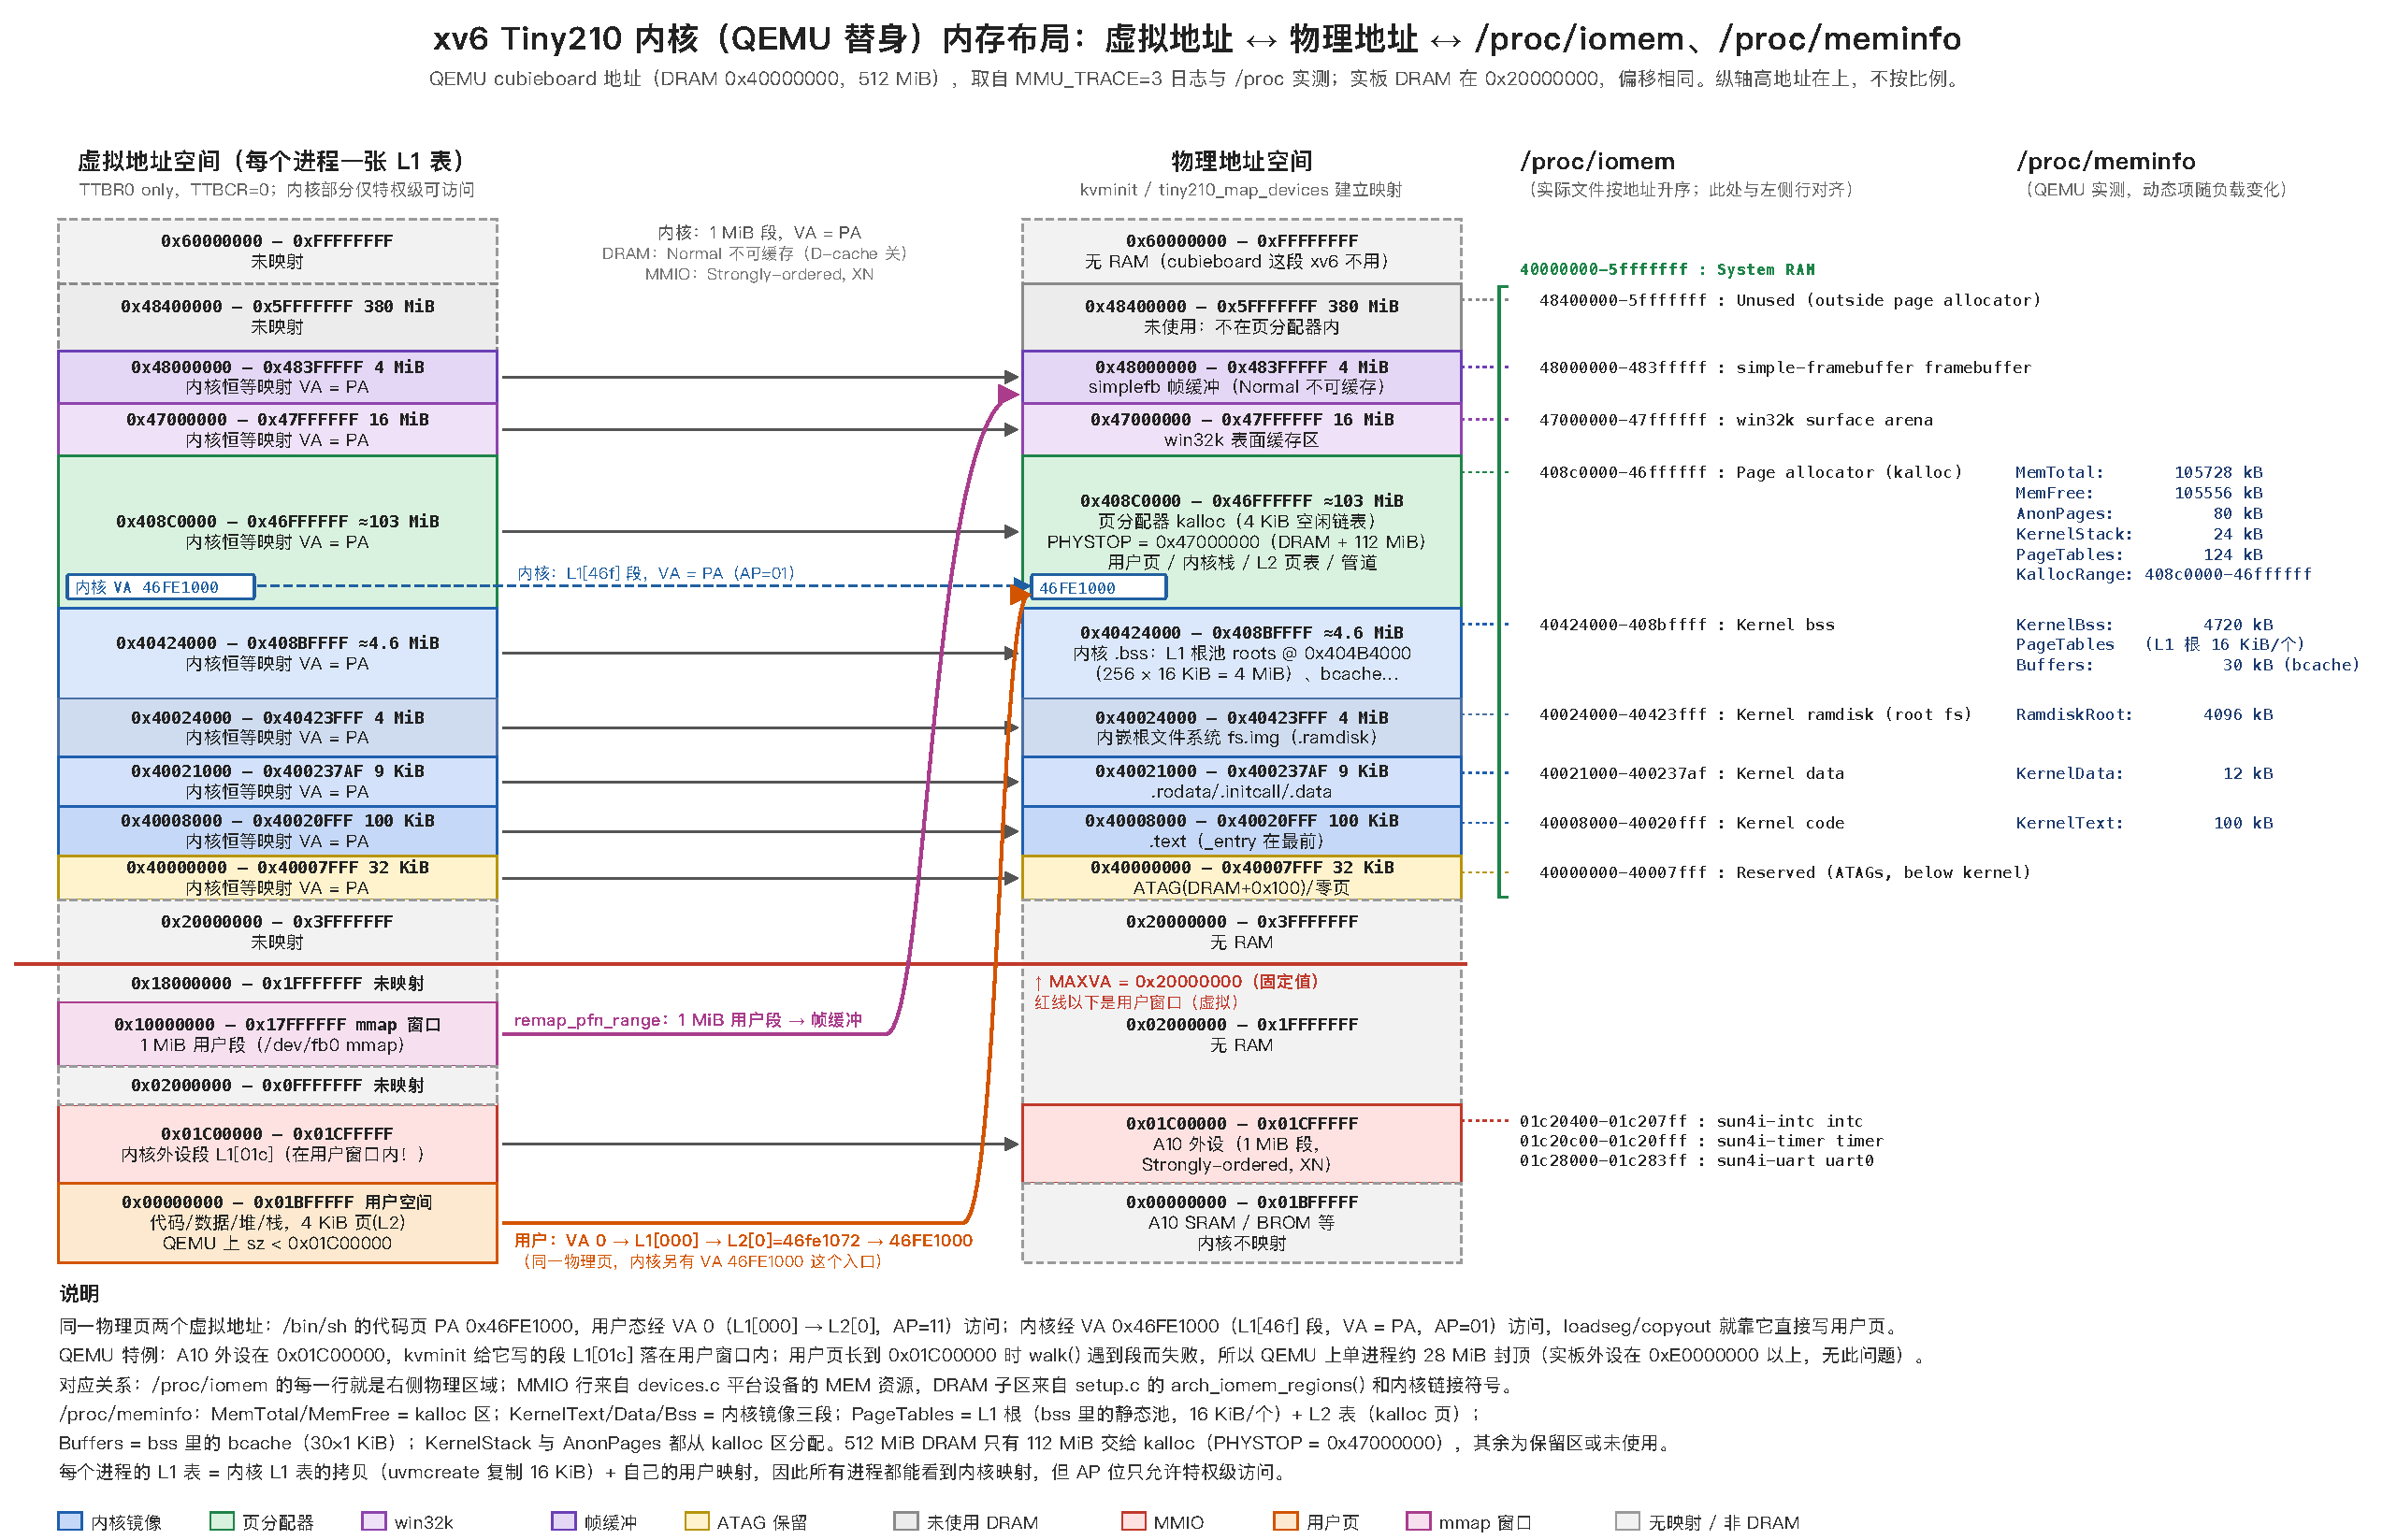
\includegraphics[width=0.92\textheight,height=\textwidth,keepaspectratio]{figures/memory-layout.pdf}}
\caption{虚拟地址 $\leftrightarrow$ 物理地址 $\leftrightarrow$ \texttt{/proc/iomem}、\texttt{/proc/meminfo}
（QEMU 地址：DRAM 从 0x40000000 开始，数值取自 MMU\_TRACE 日志与 /proc 实测；实板偏移相同、基址为 0x20000000。高地址在上，不按比例；由 \texttt{tools/memory\_layout\_svg.py} 生成）}\label{fig:memory-layout}
\end{figure}

\section{物理内存}

\begin{longtable}{@{}>{\raggedright\arraybackslash}p{0.2\textwidth}>{\raggedright\arraybackslash}p{0.37\textwidth}>{\raggedright\arraybackslash}p{0.37\textwidth}@{}}
\toprule
区域 & 实板地址 & 来源 \\
\midrule
\endhead
DRAM bank 0 & 0x20000000--0x3fffffff（512 MiB） & ATAG\_MEM（BL1 或 QEMU 传入），\texttt{board.h} 的 \texttt{BOARD\_DRAM\_SIZE} 兜底 \\
ATAG / 零页 & DRAM+0x0 -- DRAM+0x7fff & BL1 把 ATAG 放在 DRAM+0x100，内核不回收 \\
内核镜像 & 0x20008000 起 & Linux \texttt{TEXT\_OFFSET} 约定，\texttt{kernel.ld} 的 \texttt{KERNEL\_LOAD} \\
页分配器 & \texttt{end} -- DRAM+112 MiB & \texttt{setup.c}：\texttt{USE\_DRAM = S5PV210\_USE\_DRAM} \\
win32k 表面缓存区 & DRAM+112 MiB -- +128 MiB & \texttt{memlayout.h} 的 \texttt{S5PV210\_GUI\_*}，不交给 kalloc \\
LCD 帧缓冲 & DRAM+128 MiB -- +132 MiB & \texttt{devices.c} 中 s3c-fb 的 framebuffer 资源 \\
未使用 & DRAM+132 MiB -- DRAM 顶 & 约 380 MiB 闲置 \\
\bottomrule
\end{longtable}

\begin{itemize}
\item \textbf{512 MiB 中只有 112 MiB 用作通用内存。} D-cache 关闭时 \texttt{kinit} 逐页初始化很慢，
      所以 \texttt{PHYSTOP = DRAM\_BASE + 112 MiB}，ATAG 报告的其余内存不进分配器。
\item \texttt{PHYSTOP} 实际是变量 \texttt{tiny210\_phystop}：ATAG 报告的 bank 更小时会下调；
      内核本身超过它时会上调到 \texttt{end + 16 MiB}。
\end{itemize}

\section{内核镜像}

下表是实板构建的链接符号（\texttt{arm-none-eabi-nm kernel.elf}）：

\begin{longtable}{@{}>{\raggedright\arraybackslash}p{0.27\textwidth}>{\raggedright\arraybackslash}p{0.3\textwidth}>{\raggedright\arraybackslash}p{0.1\textwidth}>{\raggedright\arraybackslash}p{0.27\textwidth}@{}}
\toprule
段 & 地址 & 大小 & 内容 \\
\midrule
\endhead
Kernel code（.text） & 0x20008000--0x2002efff & 156 KiB & \texttt{\_entry} 在最前（\texttt{.text.entry}） \\
Kernel data（.rodata/.initcall/.data） & 0x2002f000--0x2003ffff & 68 KiB & 含 MT7601U 固件 45 KiB \\
Kernel bss & 0x20040000--0x20539fff & 约 5 MiB & 见下 \\
\bottomrule
\end{longtable}

bss 的大头：
\begin{itemize}
\item \texttt{roots}：\textbf{4 MiB}，256 个 16 KiB 对齐的 ARMv7 L1 页表根的静态池（\texttt{vm.c}），
      这也是地址空间个数（进程数）的上限；
\item \texttt{fw\_buf} 256 KiB、\texttt{diskmap} 256 KiB（FAT32 簇表）、\texttt{tcp\_connections} 220 KiB、
      \texttt{mt\_rx\_buf} 64 KiB；
\item \texttt{bcache}：30 个 1 KiB 块缓存（\texttt{NBUF = MAXOPBLOCKS*3}）。
\end{itemize}
QEMU 构建额外把根文件系统 \texttt{fs.img} 链接进 \texttt{.ramdisk} 段（4 MiB），位于 data 与 bss 之间。

\section{页分配器}

\texttt{kernel/kalloc.c} 是一条 4 KiB 页的单链表 freelist，一把自旋锁，没有 buddy，也没有 slab。
管理范围是 \texttt{[PGROUNDUP(end), PHYSTOP)}，实板约 0x2053a000--0x26ffffff，即
\textbf{106.8 MiB}（109336 kB）；QEMU 实测 0x408c0000--0x46ffffff = 105728 kB。

从 kalloc 取页的有：内核栈（每进程 1 页）、用户页、L2 页表、管道缓冲、\texttt{/proc} 读缓冲。
每个 L2 页表占一整页，但 ARMv7 的 L2 表只有 1 KiB，所以每张浪费 3 KiB。L1 根不来自 kalloc，
来自上面的静态池。kalloc 维护 \texttt{nfree}、\texttt{managed} 计数和 \texttt{[lo, hi)} 范围，
供 \texttt{kmemstat()} 读取，\texttt{kfreepages()} 不再遍历整条链表。

\section{MMIO 外设区}

所有 MMIO 都按 \texttt{devices.c} 平台设备表中的 MEM 资源映射为 1 MiB 段
（\texttt{tiny210\_map\_devices()}），属性是 Strongly-ordered、XN、仅特权级可访问：

\begin{longtable}{@{}>{\raggedright\arraybackslash}p{0.2\textwidth}>{\raggedright\arraybackslash}p{0.3\textwidth}>{\raggedright\arraybackslash}p{0.44\textwidth}@{}}
\toprule
设备 & 物理地址 & 说明 \\
\midrule
\endhead
s5pv210-clock & 0xE0100000（64 KiB） & 同一段里还有 SWRESET 0xE0102000、PS\_HOLD 0xE010E81C、USB\_PHY\_CONTROL \\
s5pv210-gpio / keys & 0xE0200000（4 KiB） & GPIO、EINT16--31 按键 \\
s5pv210-pwm & 0xE2500000 & 时钟源 timer3，tick 用 timer4（IRQ 25） \\
s3c2410-wdt & 0xE2700000 & 看门狗 \\
s5pv210-uart & 0xE2900000 & UART0 控制台 \\
s3c-sdhci & 0xEB000000 + 1 MiB$\times$通道 & 启动 SD 通道（由 iROM 变量 0xD0037488 决定） \\
s3c-hsotg（可选） & 0xEC000000 & \texttt{S5PV210\_USB\_OTG=1} 时启用 \\
USB PHY & 0xEC100000 & EHCI 与 OTG 共用 \\
s5p-ehci & 0xEC200000（IRQ 55） & USB-A 主机口 \\
s5pv210-vic & 0xF2000000（4 MiB） & VIC0--3 \\
s3c-fb（FIMD） & 0xF8000000 & LCD 控制器 \\
\bottomrule
\end{longtable}

BL1 运行的 iRAM（0xD0020000）只在 MMU 打开前访问，不做映射。QEMU 版换成 Allwinner A10 的外设：
intc 0x01C20400、timer 0x01C20C00、uart0 0x01C28000。

\section{虚拟地址空间}

使用 ARMv7 短描述符页表，\textbf{只用 TTBR0}（TTBCR=0）。内核与用户共用一张 L1 表，
\textbf{内核恒等映射}（\texttt{V2P(a)=a}，\texttt{KERNBASE=0}）：

\begin{lstlisting}
0x00000000 +--------------------------+
           | user text/data/heap/stack|  4 KiB pages (L2), sz < 32 MiB (uvmalloc limit)
0x02000000 +--------------------------+
           | (unmapped)               |
0x10000000 +--------------------------+
           | mmap window              |  user 1 MiB sections (/dev/fb0), shared by fork
0x18000000 +--------------------------+
           | (unmapped)               |
0x20000000 +==========================+  MAXVA = DRAM_BASE: end of the user window
           | DRAM identity (0-112 MiB)|  1 MiB sections, privileged, Normal non-cacheable
           | win32k arena, framebuffer|  1 MiB sections
0xE0000000 +--------------------------+
           | peripheral MMIO sections |  Strongly-ordered, XN, privileged
0xFFFFFFFF +--------------------------+
\end{lstlisting}

\begin{itemize}
\item \texttt{uvmcreate()} 把内核 L1 表整张（16 KiB）复制进每个进程的根，
      所以每个进程都有内核映射，靠 AP 位挡住用户态访问。
\item \texttt{\_Static\_assert(DRAM\_BASE >= MAXVA)} 保证用户窗口不会与内核恒等映射重叠；
      这也是为什么 QEMU 的 DRAM 在 0x40000000，用户窗口却仍只到 0x20000000。
\item 缓存：I-cache 和分支预测开启，\textbf{D-cache 关闭}。DRAM 段的属性是 TEX=001、C=0、B=0（Normal、不可缓存）。
      \texttt{devices.c} 里 \texttt{SECTION\_RAM} 的注释写着 ``cached Normal memory''，
      但它的位编码与 DRAM 段相同，实际同样不可缓存。
\end{itemize}

\subsection{kvminit() 图解：两级页表}

Cortex-A8 没有 LPAE，短描述符最多两级。图~\ref{fig:mmu-page-tables} 仿照 minios 的
\texttt{\_\_create\_page\_tables} 图解画出 Tiny210 的情况：左上是代码 ①--⑧，右上是两种描述符
（L1 段、L1 表描述符 + L2 小页），中间按 VA $\rightarrow$ L1 $\rightarrow$ L2 $\rightarrow$ PA 画出结果，
下面是 \texttt{install()} 的寄存器写入和注意事项。内核只用 L1 段（共 145 个：DRAM 112、win32k 16、
帧缓冲 4、MMIO 13）；用户窗口的 L1 项是 01 型表描述符，指向 \texttt{walk()} 从 kalloc 取的 L2 表，
L2 项 \texttt{PA|0x72} 映射 4 KiB 小页。

\begin{figure}[p]
\centering
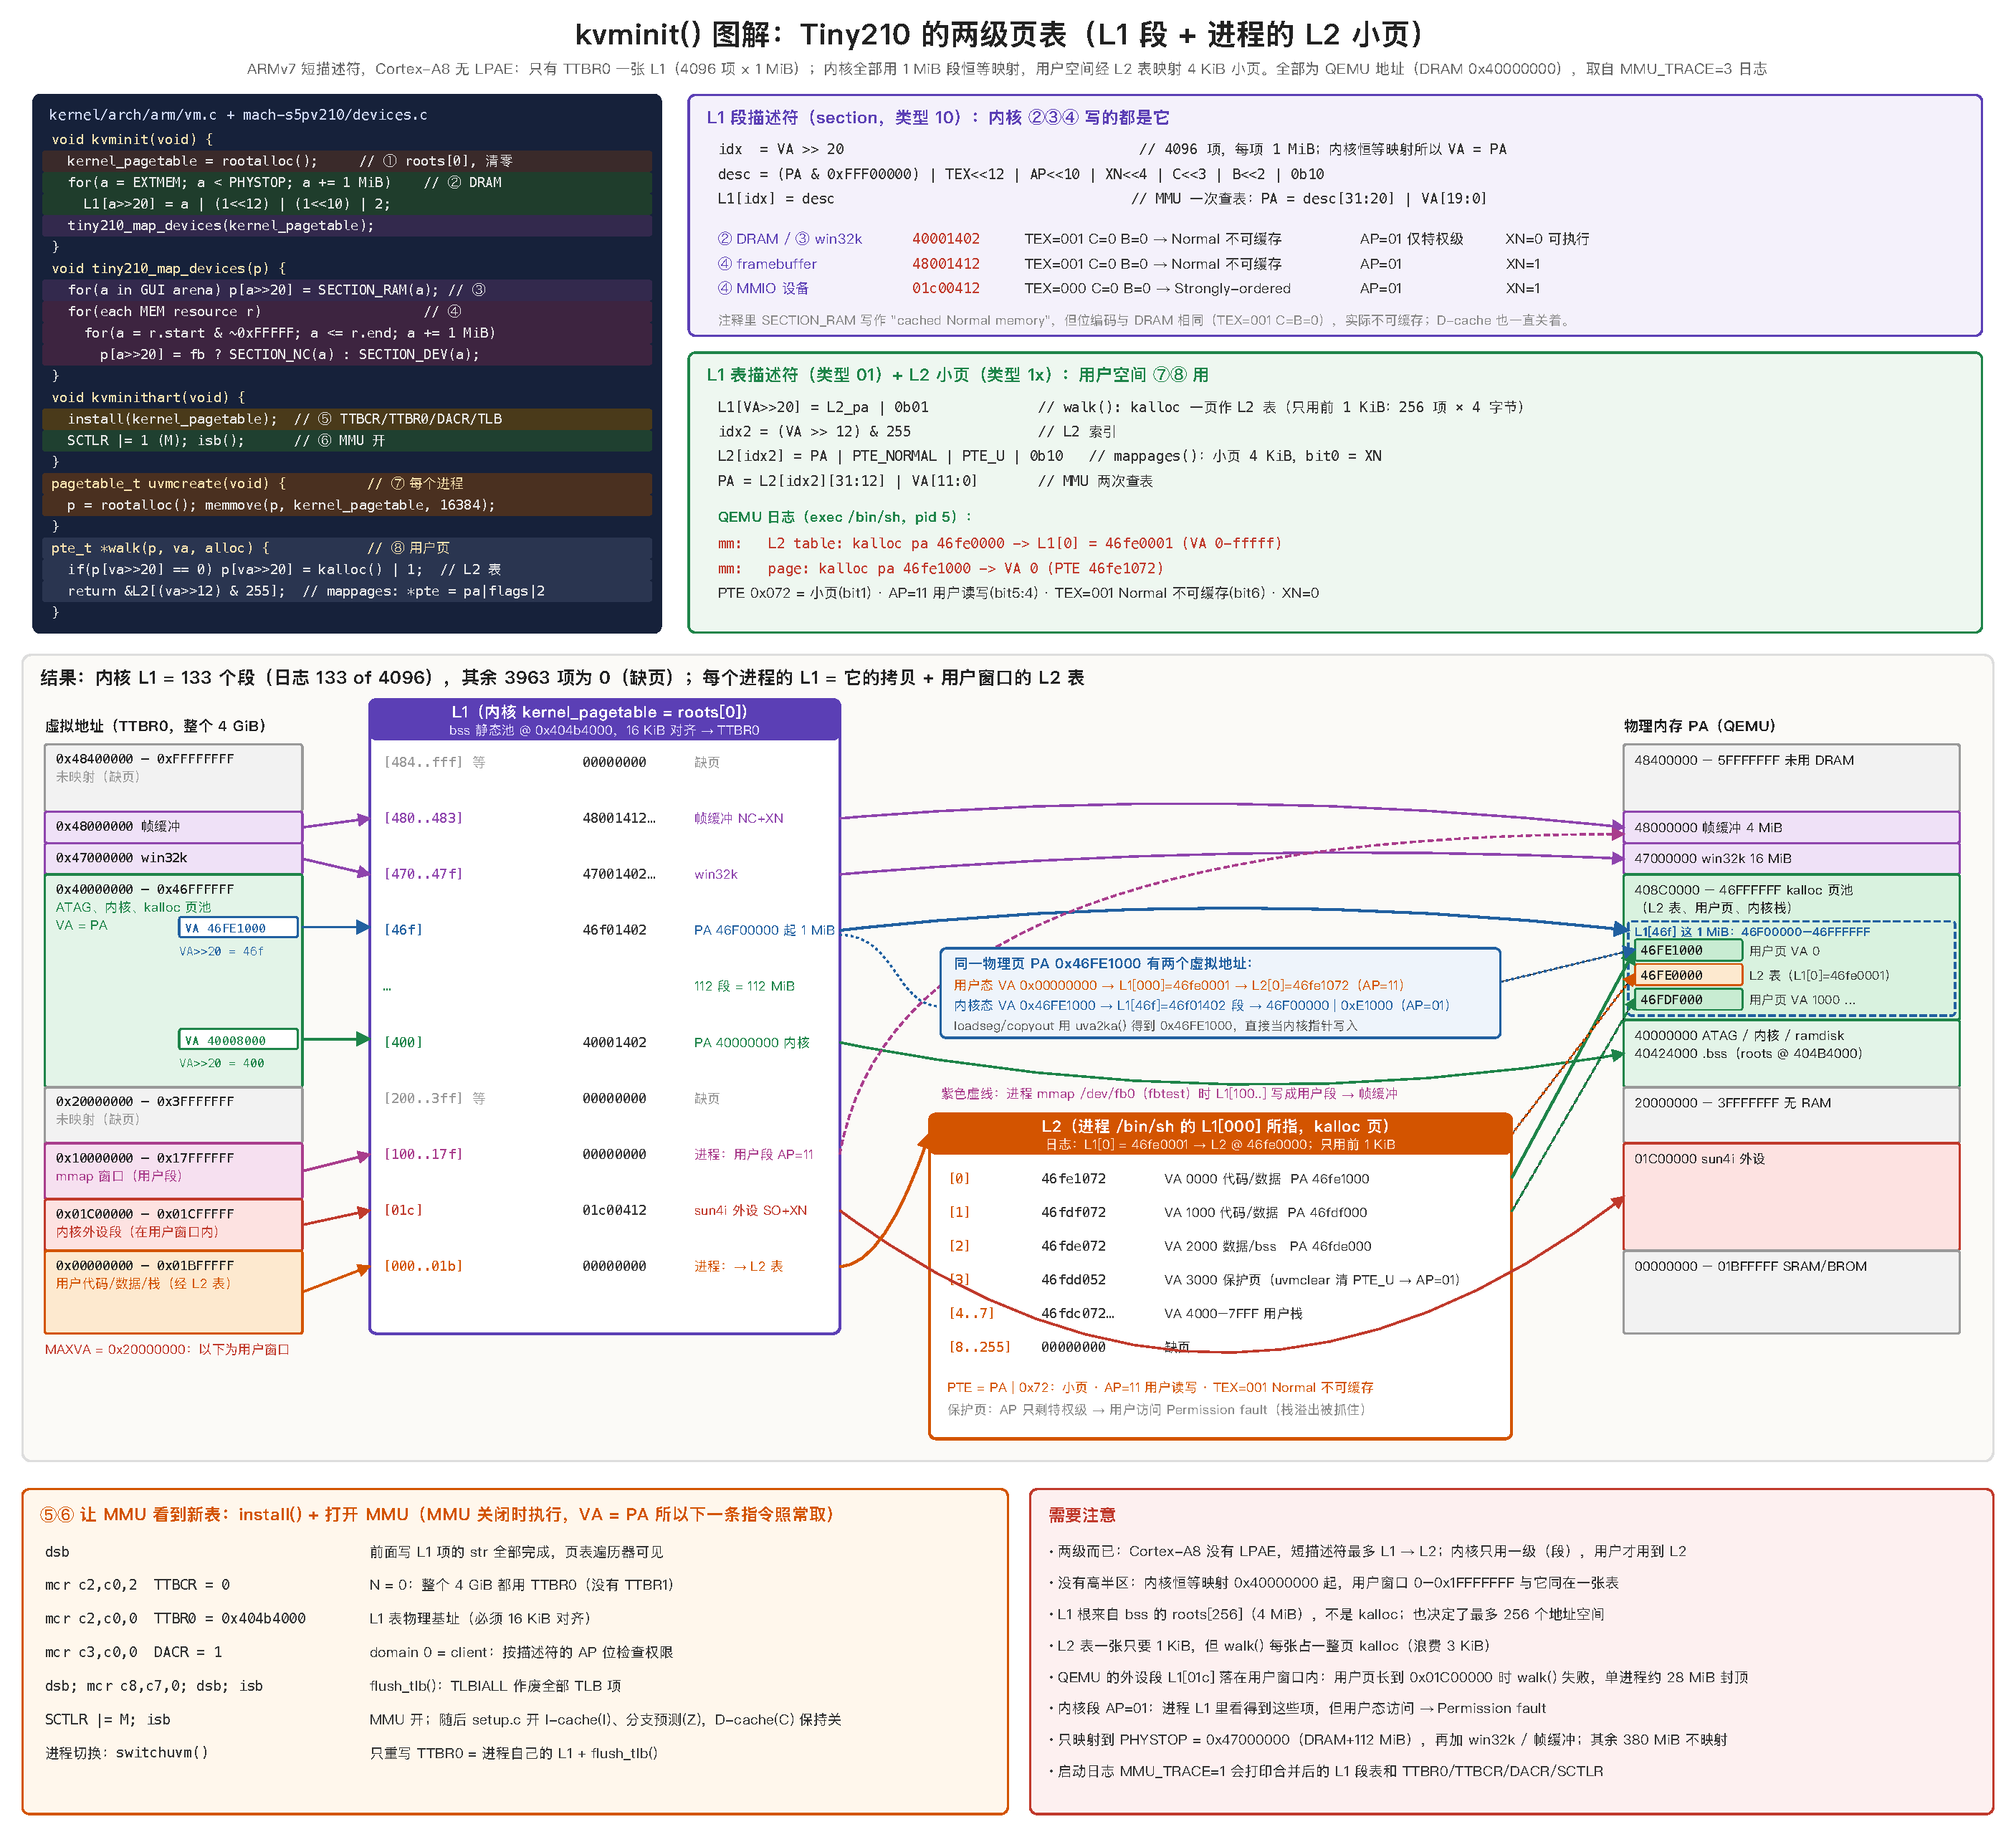
\includegraphics[width=\textwidth,height=0.92\textheight,keepaspectratio]{figures/mmu-page-tables.pdf}
\caption{kvminit() 图解：内核 L1 段与进程的 L2 小页（QEMU 地址；\texttt{tools/mmu\_page\_tables\_svg.py} 生成）}\label{fig:mmu-page-tables}
\end{figure}

\subsection{页表本身放在物理内存哪里}

\begin{itemize}
\item \textbf{内核 L1} 就是 \texttt{roots[0]}。\texttt{roots[256][4096]} 是 \texttt{vm.c} 的静态数组，位于内核
      \textbf{.bss}，不来自 kalloc：实板 roots 池在 0x200D4000--0x204D3FFF，开机 TTBR0 = 0x200D4000
      （QEMU 为 0x404B4000）。
\item \textbf{进程 L1}：\texttt{uvmcreate()} 调 \texttt{rootalloc()} 在\textbf{同一个 roots 池}里取空槽 roots[k]，
      再 \texttt{memmove} 整张 16 KiB；地址 = roots 基址 + k$\times$0x4000（QEMU 日志：/bin/sh 用 roots[6] = 0x404CC000）。
      \texttt{uvmfree} 只把 \texttt{used[k]} 清 0，不经过 kalloc。
\item \textbf{L2 表}：\texttt{walk()} 发现 L1 项为 0 时 \texttt{kalloc()} 一页，位于 \textbf{kalloc 页池}
      （实板 0x2053A000--0x26FFFFFF）。freelist 后进先出，kinit 按地址升序 kfree，表头是最高地址的页，
      所以最早分配的 L2 表和用户页紧贴 PHYSTOP 下方（QEMU：L2 在 0x46FE0000，用户页 0x46FE1000 起）。
\end{itemize}

\section{/proc/meminfo 与 /proc/iomem}

实现在 \texttt{kernel/memstat.c}，由 \texttt{kernel/vfs.c} 的 procfs 调用：
\begin{itemize}
\item \texttt{/proc/iomem} 在读取时构建资源树，按起始地址排序，按包含关系每层缩进两格。来源有四个：
      板级 RAM bank 和保留区（\texttt{setup.c} 的 \texttt{arch\_iomem\_regions()}，弱符号的默认实现是
      \texttt{EXTMEM..PHYSTOP} 一段 System RAM）；内核链接符号（code/data/bss）；kalloc 的管理范围；
      所有已注册平台设备的 MEM 资源（\texttt{device\_mem\_resources()}）。
      因此在 \texttt{devices.c} 里新增设备后，它会自动出现在 iomem 中。
\item \texttt{/proc/meminfo} 用 Linux 的 \texttt{show\_val\_kb()} 格式，后面附加若干 xv6 特有字段。
\item ARM 的 \texttt{init} 启动时执行 \texttt{mount("proc","/proc","procfs",RDONLY)}。QEMU 构建也编入了 VFS：
      没有 SD 卡时 \texttt{fat32init()} 退回内嵌 RAM 盘，\texttt{ports/tiny210/test\_shell.py} 会检查这两个文件。
\end{itemize}

\begin{longtable}{@{}>{\raggedright\arraybackslash}p{0.22\textwidth}>{\raggedright\arraybackslash}p{0.72\textwidth}@{}}
\toprule
meminfo 字段 & 含义（对应图~\ref{fig:memory-layout} 中的区域） \\
\midrule
\endhead
MemTotal & kalloc 管理的总页数（不含内核镜像和保留区，与 Linux 的含义一致） \\
MemFree / MemAvailable & freelist 上的页数 \\
Buffers & bss 中的静态块缓存 \texttt{NBUF*BSIZE} \\
AnonPages & 各进程 \texttt{vm->sz} 之和（线程与主进程共享地址空间，不重复计算） \\
KernelStack & 每进程 1 页 \\
PageTables & L1 根数 $\times$ 16 KiB + L2 表数 $\times$ 4 KiB（\texttt{vm\_pagetable\_stats()}） \\
KernelText / KernelData / KernelBss & 内核镜像三段（xv6 特有） \\
RamdiskRoot & 内嵌根文件系统大小（仅 QEMU） \\
KallocRange / Processes & 分配器物理范围、进程数 \\
\bottomrule
\end{longtable}

QEMU 实测输出：

\begin{lstlisting}
$ cat /proc/meminfo
MemTotal:         105728 kB
MemFree:          105556 kB
MemAvailable:     105556 kB
Buffers:              30 kB
Cached:                0 kB
SwapTotal:             0 kB
SwapFree:              0 kB
AnonPages:            80 kB
KernelStack:          24 kB
PageTables:          124 kB
KernelText:           96 kB
KernelData:           12 kB
KernelBss:          4724 kB
RamdiskRoot:        4096 kB
KallocRange:    408c0000-46ffffff
Processes:             6

$ cat /proc/iomem
01c20400-01c207ff : sun4i-intc intc
01c20c00-01c20fff : sun4i-timer timer
01c28000-01c283ff : sun4i-uart uart0
40000000-5fffffff : System RAM
  40000000-40007fff : Reserved (ATAGs, below kernel)
  40008000-4001ffff : Kernel code
  40020000-4002220f : Kernel data
  40023000-40422fff : Kernel ramdisk (root fs)
  40423000-408bffff : Kernel bss
  408c0000-46ffffff : Page allocator (kalloc)
  47000000-47ffffff : win32k surface arena
  48000000-483fffff : simple-framebuffer framebuffer
  48400000-5fffffff : Unused (outside page allocator)
\end{lstlisting}

实板的预期输出（尚未上板验证）：System RAM 20000000--3fffffff，下面依次是 ATAG 保留区、内核三段、
kalloc 2053a000--26ffffff、win32k 27000000--27ffffff、\texttt{s3c-fb framebuffer} 28000000--283fffff、
Unused 28400000--3fffffff，然后是上一节表中的各个 MMIO 段。

\section{MMU / 内存日志与动画}

\texttt{make ... MMU\_TRACE=n}（默认 1，定义在 \texttt{kernel/mmtrace.h}）控制以下日志，
每行以 \texttt{mm:}、\texttt{mmu:} 或 \texttt{exec:} 开头：
\begin{itemize}
\item \textbf{1 级}（启动）：DRAM 区域、内核 code/data/bss、kinit 放进空闲链表的页数、
      内核 L1 表（合并为连续的 1 MiB 段并解码属性）、TTBR0/TTBCR/DACR/SCTLR，以及整棵 \texttt{/proc/iomem}；
\item \textbf{2 级}：另加 userinit、fork、exec 的摘要（ELF LOAD 段、栈和保护页、共取了多少 kalloc 页、新 L1 根）；
\item \textbf{3 级}：另加 fork/exec 期间的每个 kalloc 页、每张 L2 页表，以及 \texttt{readi} 读入的每一块。
\end{itemize}

QEMU 下 1 级的启动片段：
\begin{lstlisting}
mm: kinit: freerange 408c0000-46ffffff -> 26432 pages (105728 KiB) on the kalloc freelist, PHYSTOP=47000000
mmu: TTBR0=404b4000 (kernel L1 root, 16 KiB aligned) TTBCR=0 DACR=1
mmu: SCTLR=c51879: M(MMU)=1 C(D-cache)=0 Z(branch pred)=1 I(I-cache)=1
mmu:   L1[1c..1c] VA 1c00000-1cfffff -> PA 1c00000  1 MiB  Strongly-ordered XN AP=1(priv RW) entry=1c00412
mmu:   L1[400..47f] VA 40000000-47ffffff -> PA 40000000  128 MiB  Normal non-cacheable AP=1(priv RW) entry=40001402
mmu:   L1[480..483] VA 48000000-483fffff -> PA 48000000  4 MiB  Normal non-cacheable XN AP=1(priv RW) entry=48001412
\end{lstlisting}

3 级下 \texttt{exec("/bin/sh")} 的片段：每个用户页先从 kalloc 取出、清零，再写 L2 PTE；
\texttt{loadseg()} 再用 \texttt{readi()} 把文件内容直接读进这个物理页：
\begin{lstlisting}
exec: /bin/sh pid 5: inode 5, 45356 bytes, ELF entry 37c, 3 program headers
mm:   L1 root roots[6] at 404cc000: copy of the kernel L1 (16 KiB, 4096 entries)
exec:   LOAD VA 0 memsz 2254 filesz 21de file off 94 flags 7
mm:   L2 table: kalloc pa 46fe0000 -> L1[0] = 46fe0001 (VA 0-fffff)
mm:   page: kalloc pa 46fe1000 -> VA 0 (PTE 46fe1072)
exec:   readi inode 5 off 94 -> VA 0 (pa 46fe1000) 4096 bytes
exec:   stack: guard page VA 3000 (PTE_U cleared), stack VA 4000-7fff
exec: /bin/sh pid 5: sz 8000 sp 7fe0 entry 37c, 9 kalloc pages, new L1 root 404cc000
\end{lstlisting}

配套动画 \texttt{doc/readme/tiny210/videos/memory-anim.mp4}（manim，约 2 分钟，
\texttt{tools/manim/memory\_anim.py}）共三段。第 1、3 段读取上面这份真实日志：内存初始化与 kinit 空闲链表；
fork + exec \texttt{/bin/sh} 时的 L1 根、L2 表、kalloc 页和 readi 加载。第 2 段按图~\ref{fig:memory-layout} 的两栏（左虚拟、右物理）讲内核 L1 表的建立，
地址全部取自 QEMU 日志（DRAM 从 0x40000000 开始）：
\begin{enumerate}
\item 短描述符格式；\texttt{rootalloc()} 取 \texttt{roots[0]}（0x404B4000）；
\item DRAM 恒等映射 L1[400..46f]，112 段，附段描述符位分解；
\item win32k L1[470..47f] 与帧缓冲 L1[480..483]（NC+XN）；
\item sun4i 外设 L1[01c]：三个寄存器块共用一段，且落在用户窗口内——用户页长到 0x01C00000 时
      \texttt{walk()} 遇到段而失败，所以 QEMU 上单进程约 28 MiB 封顶；
\item 其余项缺页（日志：133 of 4096）；\texttt{install()} 后置 SCTLR.M；两个查表实例；每个进程拷贝 L1。
\end{enumerate}
重新生成用 \texttt{tools/manim/render.sh}。

\section{可改进点}

\begin{enumerate}
\item 512 MiB 只用了 112 MiB：打开 D-cache 并做好 DMA 缓存维护后，可以把 \texttt{USE\_DRAM} 提到接近 DRAM 顶。
\item L1 根池静态占用 bss 4 MiB，可以改为按需分配 16 KiB 对齐的连续页。
\item L2 表每张占一整页却只用 1 KiB，可以 4 张合用一页。
\item \texttt{SECTION\_RAM} 的注释与实际属性不一致。
\end{enumerate}

\chapter{Tiny210 LCD、FIMD 与
framebuffer}\label{tiny210-lcdfimd-ux4e0e-framebuffer}

\section{数据通路}\label{ux6570ux636eux901aux8def}

Tiny210 的 S5PV210 FIMD 是显示控制器。CPU 把像素写进 DDR
framebuffer，FIMD 作为总线 master 周期性读取这块物理内存，再按面板时序从
RGB 引脚输出：

\begin{figure}[htbp]
\centering
\resizebox{0.90\linewidth}{!}{\begin{tikzpicture}[node distance=8mm]
  \node[hbox] (cpu) {CPU / fbcon\\写 XRGB8888};
  \node[box,right=of cpu] (ddr) {DDR framebuffer\\连续保留内存};
  \node[box,right=of ddr] (fimd) {S5PV210 FIMD\\Window 0 DMA scanout};
  \node[box,right=of fimd] (rgb) {GPF0--GPF3\\RGB/HSYNC/VSYNC/DE/PCLK};
  \node[hbox,right=of rgb] (panel) {Tiny210\\RGB LCD};
  \draw[arr] (cpu)--(ddr); \draw[arr] (ddr)--(fimd); \draw[arr] (fimd)--(rgb);
  \draw[arr] (rgb)--(panel);
\end{tikzpicture}}
\caption{CPU 绘制、FIMD 扫描和 RGB 面板输出的数据通路}
\label{fig:tiny-lcd-path}
\end{figure}


这里的``DMA''是 FIMD 自己读取 DDR，并没有单独启动通用 DMA 控制器。写入
\passthrough{\lstinline!VIDW00ADD0B0/VIDW00ADD1B0!} 的是 framebuffer
总线物理地址；当前恒等映射下， 内核指针数值与物理地址相同。

\section{资源和内存}\label{ux8d44ux6e90ux548cux5185ux5b58}

\href{../../../kernel/arch/arm/mach-s5pv210/devices.c}{\passthrough{\lstinline!devices.c!}}
给 \passthrough{\lstinline!s3c-fb!} 提供：

{\def\LTcaptype{none} % do not increment counter
\begin{longtable}[]{@{}p{0.18\linewidth}p{0.26\linewidth}p{0.50\linewidth}@{}}
\toprule\noalign{}
resource & 地址 & 作用 \\
\midrule\noalign{}
\endhead
\bottomrule\noalign{}
\endlastfoot
MEM 0 & \passthrough{\lstinline!0xF8000000..0xF800ffff!} & FIMD
寄存器 \\
MEM 1 & \passthrough{\lstinline!DRAM\_BASE + 128 MiB!}，大小 2 MiB &
连续 framebuffer \\
driver\_data & \passthrough{\lstinline!s3c\_fb\_platdata!} & 面板参数与
GPIO setup 回调 \\
\end{longtable}
}

Framebuffer 不由 \passthrough{\lstinline!kalloc()!} 动态分配，而是通过
\href{../../../kernel/arch/arm/mach-s5pv210/memlayout.h}{\passthrough{\lstinline!memlayout.h!}}
静态保留在页分配器 范围之外。\passthrough{\lstinline!setup.c!}
的静态断言防止它和 kalloc 区重叠。

800×480×4 = 1,536,000 字节，小于 2 MiB。映射属性为 privileged、Normal
non-cacheable、XN，以避免 CPU cache 与 FIMD scanout 不一致。

\section{面板选择}\label{ux9762ux677fux9009ux62e9}

编译时用 \passthrough{\lstinline!S5PV210\_LCD!} 选择
\passthrough{\lstinline!devices.c!} 的时序表：

\begin{lstlisting}[language=sh]
make -f ports/tiny210/Makefile S5PV210_BOARD=tiny210 S5PV210_LCD=s70
make -f ports/tiny210/Makefile S5PV210_BOARD=tiny210 S5PV210_LCD=h43
make -f ports/tiny210/Makefile S5PV210_BOARD=tiny210 S5PV210_LCD=w50
make -f ports/tiny210/Makefile S5PV210_BOARD=tiny210 S5PV210_LCD=a70
\end{lstlisting}

{\def\LTcaptype{none} % do not increment counter
\begin{longtable}[]{@{}p{0.18\linewidth}p{0.26\linewidth}p{0.50\linewidth}@{}}
\toprule\noalign{}
名称 & 分辨率 & 默认刷新率 \\
\midrule\noalign{}
\endhead
\bottomrule\noalign{}
\endlastfoot
S70（默认） & 800×480 & 60 Hz \\
H43 & 480×272 & 60 Hz \\
W50 & 800×480 & 60 Hz \\
A70 & 800×480 & 60 Hz \\
\end{longtable}
}

换面板后先 \passthrough{\lstinline!make tiny210-clean!}。这些参数来自
FriendlyARM BSP；实际模组若只亮背光、 图像滚动或偏移，需要对照面板
datasheet 核对 hfp/hbp/hsw、vfp/vbp/vsw 和极性。

\section{probe 配置过程}\label{probe-ux914dux7f6eux8fc7ux7a0b}

\href{../../../kernel/drivers/video/fbdev/s3c-fb.c}{\passthrough{\lstinline!s3c-fb.c!}}
的 \passthrough{\lstinline!s3c\_fb\_probe()!} 按以下顺序执行：

\begin{lstlisting}
检查 xres*yres*4 是否装得进保留 framebuffer
  -> fb_setup_gpio()
       GPF0..GPF2 全部 function 2
       GPF3[3:0] function 2
       设置驱动强度
       打开 FIMD gate
       DISPLAY_CONTROL 路由到 RGB 输出
  -> 从 clk_get_rate("hclk_dsys") 计算像素时钟分频
  -> 关闭 VIDCON0，避免配置中输出半成品
  -> 设置极性和水平/垂直时序
  -> Window 0 = XRGB8888
  -> 设置窗口坐标、大小和 line stride
  -> 设置 framebuffer start/end 总线地址
  -> 开 Window 0、ENVID、ENVID_F
  -> CPU 写彩条测试
  -> fbcon_register() 清屏并接管文本输出
\end{lstlisting}

关键寄存器关系：

\begin{lstlisting}
VIDW00ADD0B0 = framebuffer 起始物理地址
VIDW00ADD1B0 = 起始 + xres*yres*4
VIDW00ADD2   = PAGEWIDTH=xres*4, OFFSIZE=0
WINCON0      = XRGB8888 + ENWIN
VIDCON0      = pixel clock divider + ENVID/ENVID_F
\end{lstlisting}

像素时钟估算：

\begin{lstlisting}
htotal = xres + hfp + hbp + hsw
vtotal = yres + vfp + vbp + vsw
wanted_pclk = htotal * vtotal * refresh_hz
actual_pclk = hclk_dsys / (CLKVAL + 1)
\end{lstlisting}

\section{LCD 文本控制台}\label{lcd-ux6587ux672cux63a7ux5236ux53f0}

\href{../../../kernel/drivers/video/fbdev/fbcon.c}{\passthrough{\lstinline!fbcon.c!}}
提供固定 8×16 字体、浅灰前景、
深蓝背景和逐行滚屏。\passthrough{\lstinline!uartputc\_sync()!}
每输出一个字符，也调用弱符号
\passthrough{\lstinline!fbcon\_putc()!}，所以 framebuffer
注册以后串口日志和 shell 输出会同步显示在 LCD。

对于 800×480 面板，文本区是 100 列 × 30 行。输入仍来自串口，LCD
本身不提供 键盘或触摸输入路径。

\section{当前限制与改进方向}\label{ux5f53ux524dux9650ux5236ux4e0eux6539ux8fdbux65b9ux5411}

当前实现：

\begin{itemize}
\tightlist
\item
  只使用 FIMD Window 0；
\item
  单 framebuffer，CPU 和 FIMD 同时访问；
\item
  没有 page flip、双缓冲、VSYNC IRQ；
\item
  没有
  \passthrough{\lstinline!/dev/fb0!}、\passthrough{\lstinline!mmap()!}
  或用户态绘图 ABI；
\item
  没有 dirty rectangle、硬件光标、overlay；
\item
  framebuffer 是 non-cacheable，CPU 大面积绘制较慢；
\item
  背光亮度/电源没有驱动管理。
\end{itemize}

建议的演进顺序：

\begin{enumerate}
\def\labelenumi{\arabic{enumi}.}
\tightlist
\item
  添加 framebuffer device 与 \passthrough{\lstinline!ioctl!} 查询模式。
\item
  提供只映射保留 framebuffer 的受限 \passthrough{\lstinline!mmap()!}。
\item
  在 2 MiB 足够时划分 front/back buffer，并实现 page flip；800×480×4
  双缓冲 需要约 3 MiB，因此应先把保留区扩大到至少 4 MiB。
\item
  增加 FIMD VSYNC IRQ，在垂直消隐期切换缓冲，消除 tearing。
\item
  cache 打开后使用 coherent DMA 内存，或在交给 FIMD 前正确 clean cache。
\end{enumerate}

\section{故障定位}\label{ux6545ux969cux5b9aux4f4d}

{\def\LTcaptype{none} % do not increment counter
\begin{longtable}[]{@{}p{0.34\linewidth}p{0.60\linewidth}@{}}
\toprule\noalign{}
现象 & 检查 \\
\midrule\noalign{}
\endhead
\bottomrule\noalign{}
\endlastfoot
串口正常，LCD 全黑 & 面板供电/背光、FIMD
gate、DISPLAY\_CONTROL、排线方向 \\
背光亮但无图 & GPF pinmux、面板型号、framebuffer 地址、ENVID \\
有图但滚动/偏移 & porch/sync/极性/像素时钟 \\
彩条正确，文字不出现 & \passthrough{\lstinline!fbcon\_register()!}
是否执行、串口输出是否经过 \passthrough{\lstinline!uartputc\_sync()!} \\
花屏或越界 & 分辨率×4、ADD0/ADD1、PAGEWIDTH、framebuffer 保留大小 \\
QEMU 没有 LCD 日志 & \passthrough{\lstinline!tiny210-qemu!}
使用替代硬件模型，不编译
\passthrough{\lstinline!s3c-fb.c!}，这是预期行为 \\
\end{longtable}
}

% 第 5 章：Wi-Fi 驱动 + 架构总览与硬件连接（原第 6 章）+ 关联失败排查。
% 05-wifi.tex 由 tools/convert.sh 生成，不要手改；合并通过本文件 \input 完成。
\chapter{Tiny210 MT7601U USB Wi-Fi
驱动}\label{tiny210-mt7601u-usb-wi-fi-ux9a71ux52a8}

\section{当前支持范围}\label{ux5f53ux524dux652fux6301ux8303ux56f4}

Tiny210 实板构建已经把以下组件连接成一条完整链路：

\begin{lstlisting}
S5PV210 USB Host PHY1
  -> EHCI host controller（USB-A，0xEC200000，IRQ 55）
  -> USB core / usb_bus
  -> MT7601U USB driver
  -> SoftMAC 扫描、Open-System 认证、关联
  -> WPA2-PSK/CCMP 四次握手
  -> net_device "wlan0"
  -> Ethernet/ARP/IPv4/UDP/ICMP/TCP
  -> DHCP、ping 和其他 socket 用户程序
\end{lstlisting}

默认目标是高速 USB MT7601U。QEMU \passthrough{\lstinline!cubieboard!}
替身没有这套 USB host， \passthrough{\lstinline!tiny210-qemu!} 不会验证
Wi-Fi；枚举、固件、射频和真实收发必须在 Tiny210 实板测试。

主要源码：

\begin{itemize}
\tightlist
\item
  \href{../../../kernel/arch/arm/mach-s5pv210/devices.c}{\passthrough{\lstinline!devices.c!}}：PHY1、EHCI
  resource。
\item
  \href{../../../kernel/drivers/usb/host/ehci-hcd.c}{\passthrough{\lstinline!ehci-hcd.c!}}：EHCI
  枚举和 bulk 传输。
\item
  \href{../../../kernel/drivers/usb/core/usb.c}{\passthrough{\lstinline!usb.c!}}：USB
  bus、driver 匹配和 URB 生命周期。
\item
  \href{../../../kernel/drivers/net/wireless/mt7601u.c}{\passthrough{\lstinline!mt7601u.c!}}：芯片、SoftMAC、WPA2
  和 netdev。
\item
  \href{../../../kernel/drivers/net/wireless/wpa_crypto.c}{\passthrough{\lstinline!wpa\_crypto.c!}}：PBKDF2/PTK/MIC/AES
  unwrap。
\item
  \href{../../../kernel/drivers/base/firmware.c}{\passthrough{\lstinline!firmware.c!}}：\passthrough{\lstinline!request\_firmware()!}。
\item
  \href{../../../kernel/net.c}{\passthrough{\lstinline!net.c!}}：net\_device、NAPI、ARP/IP/DHCP
  和 socket 网络栈。
\item
  \href{../../../user/wifi.c}{\passthrough{\lstinline!wifi.c!}}：用户态连接命令。
\end{itemize}

\section{硬件与 USB 拓扑}\label{ux786cux4ef6ux4e0e-usb-ux62d3ux6251}

默认使用 Tiny210 底板 USB-A 口：

\begin{figure}[htbp]
\centering
\resizebox{0.90\linewidth}{!}{\begin{tikzpicture}[node distance=8mm]
  \node[hbox] (cpu) {Cortex-A8};
  \node[box,right=of cpu] (ehci) {S5PV210 EHCI\\\texttt{0xEC200000}, IRQ 55};
  \node[box,right=of ehci] (hub) {可选 High-Speed Hub};
  \node[box,right=of hub] (mt) {MT7601U USB\\bulk IN/OUT + EP0};
  \node[hbox,right=of mt] (rf) {2.4 GHz\\802.11b/g/n};
  \node[gbox,above=5mm of ehci] (phy) {USB Host PHY1\\24 MHz reference};
  \draw[arr] (cpu)--(ehci); \draw[arr] (phy)--(ehci); \draw[arr] (ehci)--(hub);
  \draw[arr] (hub)--(mt); \draw[arr] (mt)--(rf);
\end{tikzpicture}}
\caption{Tiny210 USB-A 到 MT7601U 的硬件拓扑}
\label{fig:tiny-wifi-hw}
\end{figure}


\passthrough{\lstinline!host\_phy\_init()!} 会：

\begin{enumerate}
\def\labelenumi{\arabic{enumi}.}
\tightlist
\item
  打开 USBHOST 时钟 gate；
\item
  解除 PHY1 isolation；
\item
  选择 24 MHz reference；
\item
  清 PHY1 suspend/power-down；
\item
  pulse PHY1 和 host link reset。
\end{enumerate}

EHCI device resource 是：

{\def\LTcaptype{none} % do not increment counter
\begin{longtable}[]{@{}p{0.34\linewidth}p{0.60\linewidth}@{}}
\toprule\noalign{}
资源 & 值 \\
\midrule\noalign{}
\endhead
\bottomrule\noalign{}
\endlastfoot
EHCI MMIO & \passthrough{\lstinline!0xEC200000..0xEC2fffff!} \\
IRQ & 55（\passthrough{\lstinline!uhost!}） \\
USB PHY MMIO & \passthrough{\lstinline!0xEC100000..0xEC100fff!} \\
\end{longtable}
}

\section{USB/Wi-Fi 分层 Trace 开关}\label{tiny210-wifi-trace}

Tiny210 构建提供一个总开关和五个可独立覆盖的分层开关。一次打开 USB
探测、枚举、传输以及 MT7601U 配置和数据路径：

\begin{lstlisting}[language=sh]
make tiny210 USB_WIFI_TRACE=1
\end{lstlisting}

等级 2 进一步打开逐寄存器和逐 802.11 帧日志。若只编译镜像、不执行 SD
卡安装流程，可直接指定 Tiny210 Makefile 的镜像目标：

\begin{lstlisting}[language=sh]
make tiny210 USB_WIFI_TRACE=2
make -f ports/tiny210/Makefile USB_WIFI_TRACE=1 \
  build/tiny210/xv6-tiny210.uImage
\end{lstlisting}

\begingroup\small
\begin{longtable}{p{35mm}p{24mm}p{73mm}}
\toprule
开关 & 日志前缀 & 覆盖阶段 \\ \midrule \endhead
{\ttfamily\scriptsize USB\_CORE\_TRACE} & {\ttfamily\scriptsize usb-core:} & device/driver 注册、ID 匹配、probe/remove \\
{\ttfamily\scriptsize USB\_ENUM\_TRACE} & {\ttfamily\scriptsize usb-enum:} & EHCI 根口、Hub、描述符、地址和端点枚举 \\
{\ttfamily\scriptsize USB\_XFER\_TRACE} & {\ttfamily\scriptsize usb-xfer:} & control/bulk、QH/qTD、RX arm/completion 和 IRQ \\
{\ttfamily\scriptsize MT7601U\_\allowbreak CONFIG\_\allowbreak TRACE=1} & {\ttfamily\scriptsize wifi-config:} & 固件、eFuse、MAC/BBP/RF、校准和状态机 \\
{\ttfamily\scriptsize MT7601U\_\allowbreak CONFIG\_\allowbreak TRACE=2} & {\ttfamily\scriptsize wifi-reg:} & 在配置跟踪上增加逐寄存器访问 \\
{\ttfamily\scriptsize MT7601U\_\allowbreak DATA\_\allowbreak TRACE=1} & {\ttfamily\scriptsize wifi-data:} & TX/RX、NAPI、Ethernet 与 USB 缓冲流转 \\
{\ttfamily\scriptsize MT7601U\_\allowbreak DATA\_\allowbreak TRACE=2} & {\ttfamily\scriptsize wifi-frame:} & 在数据跟踪上增加逐 802.11 帧摘要 \\
\bottomrule
\end{longtable}
\endgroup

总开关只是五项的默认值，因此可以打开总体跟踪后单独关闭最密集的 EHCI
传输日志：

\begin{lstlisting}[language=sh]
make tiny210 USB_WIFI_TRACE=1 USB_XFER_TRACE=0
\end{lstlisting}

日志前缀与函数调用链的关系如下：

\begin{lstlisting}
ehci_enumerate_device
  -> usb-enum: descriptor/address/config/endpoint
  -> usb_device_register
     -> usb-core: match 148f:7601 -> mt7601u_probe
        -> wifi-config: firmware/eFuse/MAC/BBP/RF/calibration
           -> usb-xfer: EP0/EP8/EP4/EP5 QH and qTD

EHCI IRQ 55
  -> usb-xfer: EP4 completion
  -> mt7601u_rx_irq -> NAPI -> mt7601u_rx_parse
     -> wifi-data: Ethernet/NAPI path
     -> wifi-frame: each 802.11 frame (level 2 only)
\end{lstlisting}

错误、超时和初始化结果不受 Trace 开关影响。构建系统把当前五项取值写入
\passthrough{\lstinline!build/tiny210/.usb-wifi-trace!}；任一值变化都会自动重编译
\passthrough{\lstinline!usb.c!}、\passthrough{\lstinline!ehci-hcd.c!} 和
\passthrough{\lstinline!mt7601u.c!}，无需先执行
\passthrough{\lstinline!make clean!}。

根口上的 full/low-speed 设备需要 OHCI，当前没有 OHCI 驱动；高速 MT7601U
可直接由 EHCI 管理。也可以通过
\passthrough{\lstinline!S5PV210\_USB\_OTG=1!} 编入 OTG/DWC2 host
device，但默认 Wi-Fi 路径是 USB-A/EHCI。

\section{构建、firmware
和配置文件}\label{ux6784ux5efafirmware-ux548cux914dux7f6eux6587ux4ef6}

实板 \passthrough{\lstinline!ports/tiny210/Makefile!} 会编入：

\begin{lstlisting}
usb/core/usb
usb/host/ehci-hcd
usb/dwc2/hcd
net/wireless/mt7601u
net/wireless/wpa_crypto
base/firmware
net + workqueue + epoll + sysnet
wifi + dhcp + ping 用户程序
\end{lstlisting}

固件文件必须存在于仓库的：

\begin{lstlisting}
firmware/mt7601u.bin
\end{lstlisting}

构建会把它链接到内核，并在 \passthrough{\lstinline!make tiny210!}
时复制到已挂载的 FAT32 bootfs：

\begin{lstlisting}
/Volumes/bootfs/mt7601u.bin
\end{lstlisting}

\passthrough{\lstinline!request\_firmware("mt7601u.bin")!} 的优先级是：

\begin{lstlisting}
FAT32 根目录 /boot/mt7601u.bin
  -> 找不到或不可读
内核镜像中的 fw_mt7601u_start..fw_mt7601u_end
\end{lstlisting}

这样可以只替换 SD 卡上的固件进行测试，同时保留内置副本作为启动兜底。

可选 Wi-Fi 配置文件默认位于：

\begin{lstlisting}
ports/tiny210/wifi.conf
\end{lstlisting}

内容：

\begin{lstlisting}
ssid=your-access-point
psk=your-passphrase
\end{lstlisting}

该文件被 \passthrough{\lstinline!.gitignore!} 排除。构建发现它时，通过
\passthrough{\lstinline!mkfs --etc!} 写入根文件系统的
\passthrough{\lstinline!/etc/wifi.conf!}。不要把真实密码提交到仓库。

\section{initcall、枚举与驱动匹配}\label{initcallux679aux4e3eux4e0eux9a71ux52a8ux5339ux914d}

初始化顺序依靠 initcall level 和 order：

\begin{lstlisting}
netinit()                         注册 net bus
subsys_initcall("usbcore")       注册 usb bus
module_init_ord("mt7601u", 1)   注册 USB driver，建立 mt7601u_wq
module_init_ord("ehci-s5p", 2)  probe EHCI，申请 IRQ55，创建 ehci-enum
scheduler()                       CPU IRQ 打开，内核线程开始运行
ehci-enum                         PHY/host 初始化并枚举设备
\end{lstlisting}

EHCI 枚举流程：

\begin{figure}[htbp]
\centering
\resizebox{\linewidth}{!}{\begin{tikzpicture}[node distance=5mm]
  \node[hbox] (host) {EHCI host/PHY 初始化};
  \node[box,right=of host] (reset) {Port reset\\GET\_DESCRIPTOR(8)};
  \node[box,right=of reset] (addr) {SET\_ADDRESS\\读取 device/config};
  \node[box,right=of addr] (ep) {解析 bulk endpoint\\SET\_CONFIGURATION};
  \node[box,right=of ep] (bus) {\texttt{usb\_device\_register()}};
  \node[hbox,right=of bus] (probe) {VID:PID 匹配\\\texttt{mt7601u\_probe()}};
  \draw[arr] (host)--(reset); \draw[arr] (reset)--(addr); \draw[arr] (addr)--(ep);
  \draw[arr] (ep)--(bus); \draw[arr] (bus)--(probe);
\end{tikzpicture}}
\caption{EHCI 枚举 MT7601U 并交给 USB driver 的过程}
\label{fig:tiny-wifi-enum}
\end{figure}


MT7601U ID 表包含 \passthrough{\lstinline!148f:7601!} 以及多个 OEM
VID:PID。USB core 使用 ID table 匹配，不依赖设备名。EHCI
枚举在内核线程而不是 initcall 中完成，是因为端口上电、 reset
和描述符事务会等待数百毫秒，需要调度器、timer 和 IRQ 已可用。

\section{\texorpdfstring{\texttt{mt7601u\_probe()}
初始化阶段}{mt7601u\_probe() 初始化阶段}}\label{mt7601u_probe-ux521dux59cbux5316ux9636ux6bb5}

probe 的主要阶段如下：

\begin{figure}[htbp]
\centering
\begin{tikzpicture}[node distance=6mm]
  \node[hbox] (p) {\texttt{mt7601u\_probe}};
  \node[box,below=of p] (ver) {vendor control\\读取 ASIC/MAC version};
  \node[box,below=of ver] (fw) {校验并下载 firmware\\ILM + DLM + IVB};
  \node[box,below=of fw] (mcu) {等待 MCU running\\读取 256 B eFuse};
  \node[box,below=of mcu] (init) {WLAN PLL、MAC、USB DMA\\MAC/BBP/RF 表与校准};
  \node[hbox,below=of init] (rx) {channel 1，提交 4 个 RX buffer\\启动 delayed scan work};
  \draw[arr] (p)--(ver); \draw[arr] (ver)--(fw); \draw[arr] (fw)--(mcu);
  \draw[arr] (mcu)--(init); \draw[arr] (init)--(rx);
\end{tikzpicture}
\caption{MT7601U probe 的主要硬件初始化阶段}
\label{fig:tiny-wifi-probe}
\end{figure}


\subsection{控制传输}\label{ux63a7ux5236ux4f20ux8f93}

MT7601U 寄存器不是 CPU MMIO。驱动通过 USB vendor control request 读写：

\begin{lstlisting}
mt7601u_read32/write32
  -> udev->ops->control
  -> EHCI EP0 SETUP/DATA/STATUS qTD
  -> MT7601U vendor request
\end{lstlisting}

\subsection{固件下载}\label{ux56faux4ef6ux4e0bux8f7d}

固件头给出 ILM/DLM 长度。驱动把数据按最大
\passthrough{\lstinline!0x3800!} 字节分块，增加 FCE TXINFO， 通过
bulk-OUT 下载：

\begin{lstlisting}
ILM: 目的地址从 64 B IVB 之后开始
DLM: 目的地址 0x80000
最后: DEV_MODE=0x12 携带 64 B IVB，启动 MCU
\end{lstlisting}

每块之后检查 FCE/MCU 状态，最后轮询
\passthrough{\lstinline!MCU\_COM\_REG0 == 1!}。

\subsection{eFuse
和射频初始化}\label{efuse-ux548cux5c04ux9891ux521dux59cbux5316}

驱动读取 256 字节 eFuse，获得永久 MAC、country、晶振 frequency
offset、RSSI offset、参考温度和 LNA gain。随后初始化 MAC、BBP、RF
表，并通过 MCU command endpoint 执行 R、TXDCOC、LOFT、TXIQ、RXIQ 和 DPD
等校准。

任何阶段失败都会使 probe 返回失败，\passthrough{\lstinline!wlan0!}
不会出现。

\section{扫描、认证和 WPA2
状态机}\label{ux626bux63cfux8ba4ux8bc1ux548c-wpa2-ux72b6ux6001ux673a}

\passthrough{\lstinline!/bin/wifi!} 最终调用：

\begin{lstlisting}
wifi_connect(ssid, psk)
  -> SYS_wifi_connect
  -> sys_wifi_connect()
  -> mt7601u_connect(ssid, psk, 30000)
\end{lstlisting}

\passthrough{\lstinline!mt7601u\_connect()!} 在进程上下文执行 PBKDF2
4096 轮生成 32 字节 PMK，然后设置 目标 SSID，唤醒
\passthrough{\lstinline!mt7601u\_wq!} 的 delayed work，并睡眠等待最多 30
秒。

\begin{figure}[htbp]
\centering
\resizebox{\linewidth}{!}{\begin{tikzpicture}[node distance=6mm]
  \node[hbox] (scan) {SCAN\\channel 1--11};
  \node[box,right=of scan] (authp) {AUTH\_PENDING};
  \node[box,right=of authp] (auth) {AUTH\_SENT};
  \node[box,right=of auth] (assocp) {ASSOC\_PENDING};
  \node[box,right=of assocp] (assoc) {ASSOC\_SENT};
  \node[box,right=of assoc] (eapol) {ASSOCIATED\\EAPOL M1--M4};
  \node[hbox,right=of eapol] (key) {KEYED\\注册 \texttt{wlan0}};
  \draw[arr] (scan)--node[lab,above]{命中 SSID}(authp);
  \draw[arr] (authp)--(auth); \draw[arr] (auth)--(assocp); \draw[arr] (assocp)--(assoc);
  \draw[arr] (assoc)--(eapol); \draw[arr] (eapol)--(key);
  \draw[darr,bend right=35] (auth) to node[lab,below]{timeout} (authp);
  \draw[darr,bend right=38] (eapol) to node[lab,below]{watchdog} (assocp);
\end{tikzpicture}}
\caption{扫描、Open-System 认证、关联与 WPA2 状态机}
\label{fig:tiny-wifi-state}
\end{figure}


扫描在 2.4 GHz channel 1..11 间切换，每个 channel 解析 beacon/probe
response， 最多保存 32 个 AP。WPA2 四次握手中：

\begin{enumerate}
\def\labelenumi{\arabic{enumi}.}
\tightlist
\item
  收到 M1：保存 ANonce，生成 SNonce，PMK 派生 PTK，发送 M2；
\item
  收到 M3：校验 MIC，AES unwrap key data，提取 GTK；
\item
  把 PTK/GTK 写进 MT7601U hardware key tables，启用 AES-CCMP；
\item
  发送 M4，设置 \passthrough{\lstinline!handshake\_done!}。
\end{enumerate}

当前实现面向 WPA2-PSK/CCMP。没有完整支持
WPA3、802.1X/EAP、WEP、WPA-TKIP、 5 GHz、11n 高级速率控制或省电模式。

\section{RX：IRQ + NAPI
风格下半部}\label{rxirq--napi-ux98ceux683cux4e0bux534aux90e8}

probe 会在数据 bulk-IN endpoint 预提交 4 个 16 KiB buffer。数据到达时：

\begin{figure}[htbp]
\centering
\resizebox{\linewidth}{!}{\begin{tikzpicture}[node distance=5mm]
  \node[hbox] (mt) {MT7601U\\bulk-IN complete};
  \node[box,right=of mt] (irq) {EHCI IRQ55\\确认 qTD 状态};
  \node[box,right=of irq] (napi) {\texttt{mt7601u\_rx\_irq}\\调度 NAPI work};
  \node[box,right=of napi] (parse) {解析 RXWI / 802.11\\立即重提 RX buffer};
  \node[box,right=of parse] (kind) {管理帧/EAPOL 驱动内处理\\数据帧重建 Ethernet};
  \node[hbox,right=of kind] (net) {\texttt{net\_rx\_dev()}\\ARP/IP/UDP/TCP};
  \draw[arr] (mt)--(irq); \draw[arr] (irq)--(napi); \draw[arr] (napi)--(parse);
  \draw[arr] (parse)--(kind); \draw[arr] (kind)--(net);
\end{tikzpicture}}
\caption{Wi-Fi RX 从 EHCI 中断到 xv6 网络栈}
\label{fig:tiny-wifi-rx}
\end{figure}


硬中断只确认 EHCI 状态并调度 NAPI work，不在 IRQ 上下文解析
beacon、EAPOL 或 IP。 NAPI 每轮 budget 是 4；若一次用满
budget，workqueue 会继续调度。状态机的 timeout 使用独立
\passthrough{\lstinline!state\_work!}，因此 RX completion
与协议定时器互不阻塞。

\section{TX 与网络栈}\label{tx-ux4e0eux7f51ux7edcux6808}

网络栈交给 \passthrough{\lstinline!mt7601u\_net\_xmit()!} 的是 Ethernet
frame。驱动会：

\begin{enumerate}
\def\labelenumi{\arabic{enumi}.}
\tightlist
\item
  根据目标/源 MAC 和 EtherType 构造 802.11 ToDS header；
\item
  添加 LLC/SNAP；
\item
  关联后选择 AP 的 WCID；
\item
  握手完成后让硬件使用已安装的 CCMP key；
\item
  添加 MT7601U TXWI 和 USB DMA header；
\item
  通过 bulk-OUT 同步发送。
\end{enumerate}

RX 数据路径反向去掉 RXWI、802.11 header 和 LLC/SNAP，重建 Ethernet
header 后调用
\passthrough{\lstinline!net\_rx\_dev()!}。握手完成以前，普通数据 frame
不会交给 IP 层。

驱动注册的真实接口名是
\passthrough{\lstinline!wlan0!}。当前一条日志仍写成
\passthrough{\lstinline!wlan1 registered!}，这是日志
字符串遗留，不代表存在第二个接口；DHCP 应使用
\passthrough{\lstinline!wlan0!}。

\section{自动连接和手工测试}\label{ux81eaux52a8ux8fdeux63a5ux548cux624bux5de5ux6d4bux8bd5}

如果根文件系统有 \passthrough{\lstinline!/etc/wifi.conf!}，Tiny210
\passthrough{\lstinline!/init!} 会后台重试连接最多 10 次；
\passthrough{\lstinline!wifi!} 成功后执行：

\begin{lstlisting}[language=sh]
/bin/dhcp wlan0
\end{lstlisting}

手工连接：

\begin{lstlisting}[language=sh]
/bin/wifi YOUR_SSID YOUR_PASSPHRASE
/bin/dhcp wlan0
/bin/ping 192.168.0.1
\end{lstlisting}

也可直接让 \passthrough{\lstinline!wifi!} 读取配置：

\begin{lstlisting}[language=sh]
/bin/wifi
/bin/dhcp wlan0
\end{lstlisting}

成功的关键日志顺序通常是：

\begin{lstlisting}
ehci: high-speed device 148f:7601 ...
mt7601u: USB device 148f:7601 ASIC=...
firmware: mt7601u.bin loaded from /boot (... bytes)
mt7601u: MCU firmware running
mt7601u: permanent mac=...
mt7601u: MAC/BBP/RF bootstrap ready
mt7601u: RF calibration complete; bulk endpoints ready
mt7601u: target <ssid> found ... WPA2
mt7601u: Open-System authentication accepted
mt7601u: 802.11 associated ...
mt7601u: WPA2 four-way handshake complete
mt7601u: wlan1 registered ...     # 实际接口名 wlan0
dhcp: dev=wlan0 address=... gateway=... dns=...
\end{lstlisting}

\section{当前已知限制}\label{ux5f53ux524dux5df2ux77e5ux9650ux5236}

\begin{itemize}
\tightlist
\item
  只维护一个全局 \passthrough{\lstinline!mt7601u\_device!}，不支持多块
  MT7601U。
\item
  EHCI 启动只在约 2
  秒窗口内寻找设备，之后枚举线程永久睡眠；\textbf{不支持 USB 热插拔}。
  网卡应在启动前插好。
\item
  根口 full/low-speed 设备交给尚未实现的 OHCI；MT7601U 必须以 high-speed
  工作。
\item
  扫描只覆盖 channel 1..11，没有根据 country 自动扩大/缩小 regulatory
  domain。
\item
  \passthrough{\lstinline!mt7601u\_send\_assoc()!} 当前 association
  request 中仍有硬编码
  \passthrough{\lstinline!TP-Link\_B114!}，虽然扫描和
  \passthrough{\lstinline!wifi\_connect()!} 接受任意 SSID；连接其他 SSID
  前应把 这里改成
  \passthrough{\lstinline!dev->want\_ssid/dev->want\_ssid\_len!}。
\item
  TX bulk 是同步路径；高吞吐时会占用调用进程，尚无完整 TX
  queue/backpressure。
\item
  驱动没有 Linux mac80211/cfg80211 的速率控制、重连、扫描 API
  和监管框架。
\item
  D-cache 当前关闭，简化了 EHCI DMA 一致性；以后开启 D-cache 时必须补齐
  DMA coherent allocation 或 cache clean/invalidate。
\item
  Wi-Fi 配置是明文文件，系统没有密钥环或权限隔离。
\end{itemize}

\section{故障定位}\label{ux6545ux969cux5b9aux4f4d}

{\def\LTcaptype{none} % do not increment counter
\begin{longtable}[]{@{}p{0.34\linewidth}p{0.60\linewidth}@{}}
\toprule\noalign{}
最后日志/现象 & 优先检查 \\
\midrule\noalign{}
\endhead
\bottomrule\noalign{}
\endlastfoot
没有 \passthrough{\lstinline!initcall: ehci-s5p!} & 实板构建是否误用了
\passthrough{\lstinline!QEMU\_TEST=1!} \\
\passthrough{\lstinline!no high-speed device!} &
网卡是否开机前插入、USB-A 供电、PHY1/时钟、是否被识别为 full-speed \\
有 VID:PID，没有 probe & ID 是否在
\passthrough{\lstinline!mt7601u\_ids[]!}、usbcore/driver initcall
顺序 \\
\passthrough{\lstinline!firmware ... missing!} &
\passthrough{\lstinline!/boot/mt7601u.bin!} 和内置
\passthrough{\lstinline!firmware/mt7601u.bin!} \\
\passthrough{\lstinline!MCU firmware start timeout!} & bulk-OUT、FCE
地址/长度、固件版本、USB 错误 token \\
\passthrough{\lstinline!calibration ... failed!} & 第二 bulk-IN MCU
response endpoint、eFuse/RF、供电和 USB 稳定性 \\
能扫描但认证超时 & channel、BSSID、AP 是否允许 Open-System auth、USB RX
completion \\
关联后 M1 timeout & AP 安全模式应为 WPA2-PSK/CCMP，检查 EAPOL RX 和
receive filter \\
\passthrough{\lstinline!M3 MIC verification failed!} & 密码错误、PMK/PTK
派生或 replay/nonce \\
\passthrough{\lstinline!wifi: associated!} 但 DHCP 失败 & 使用
\passthrough{\lstinline!wlan0!}、ARP/DHCP response 是否进入
\passthrough{\lstinline!net\_rx\_dev()!} \\
一直连不上非 TP-Link\_B114 & 当前 association request 的硬编码 SSID
限制 \\
\end{longtable}
}

% 本章由手工维护（不由 tools/convert.sh 生成），内容与 doc/readme/tiny210/wifi-architecture.md 同步。
% 05a/05b/05c 三章共用下面的样式；名字加 w 前缀，避免和书稿自身的 box/arr/darr/lab 冲突。
\usetikzlibrary{backgrounds}
\providecommand{\fn}[1]{{\ttfamily\small #1}}
\definecolor{wamber}{RGB}{176,112,20}
\definecolor{wgray}{RGB}{110,118,126}
\tikzset{
  wbox/.style={draw=#1,fill=#1!8,rounded corners=2pt,align=center,font=\small,inner sep=4pt,minimum height=8mm},
  wbox/.default=tinyblue,
  wlayer/.style={draw=#1,fill=#1!8,rounded corners=2pt,minimum width=140mm,minimum height=9mm,align=left,font=\small,text width=136mm},
  warr/.style={-{Stealth[length=2.2mm]},thick,draw=wgray},
  wdarr/.style={{Stealth[length=2.2mm]}-{Stealth[length=2.2mm]},thick,draw=wgray},
  wlbl/.style={font=\scriptsize,fill=white,inner sep=1pt},
}
\providecommand{\seqhead}[3]{\node[wbox=tinyblue,minimum width=22mm,font=\footnotesize] (#2) at (#1,0) {#3};}
\providecommand{\seqline}[2]{\draw[dashed,wgray] (#1,-0.45) -- (#1,-#2);}
\providecommand{\seqmsg}[4]{\draw[-{Stealth[length=2mm]},thick,tinyblue] (#1,-#3) -- node[above,font=\scriptsize,inner sep=1pt]{#4} (#2,-#3);}
\providecommand{\seqret}[4]{\draw[-{Stealth[length=2mm]},thick,dashed,tinygreen] (#1,-#3) -- node[above,font=\scriptsize,inner sep=1pt]{#4} (#2,-#3);}
\providecommand{\seqself}[3]{\draw[-{Stealth[length=2mm]},thick,wamber] (#1,-#2) -- ++(0.35,0) -- ++(0,-0.3) -- ++(-0.35,0);
  \node[right,font=\scriptsize,align=left] at (#1+0.4,-#2-0.15) {#3};}
\providecommand{\seqnote}[4]{\node[draw=wamber,fill=wamber!10,font=\scriptsize,anchor=north west,inner sep=2pt] at (#1,-#3) {#4};}

\chapter{MT7601U Wi-Fi 架构总览与硬件连接}\label{wa:ch-05a-wifi-arch-hw}
\section{概述}

第~\ref{tiny210-mt7601u-usb-wi-fi-ux9a71ux52a8} 章讲了 MT7601U 驱动的使用、构建和故障定位。本章和后面两章换一个角度，把这条链路逐层拆开：结合 rpi3-lock 分支 xv6-book 的 MT7601U 章节，说明 Tiny210 上 xv6 的 USB Wi-Fi 链路：一个 MT7601U USB 网卡从插在
SDK 底板 USB-A Host 口开始，到用 WPA2 连上 TP-Link\_B114 路由器、DHCP 拿到 IP 为止，
每一层用的是哪个驱动、哪个函数，以及实板串口上对应打印哪一行日志。文中的日志都是
2026-11-14 在实板上抓到的真实输出。三章内容和
\fn{doc/readme/tiny210/wifi-architecture.md} 同步。

和 Linux 一样，整个链路按“谁只关心哪一层”切开：用户态只看到“连接 / DHCP / ping”；
\fn{net.c} 只看到一个能收发 Ethernet 帧的 \fn{wlan0}；\fn{mt7601u.c} 把 Ethernet 帧
翻译成 802.11 帧并管理连接状态；\fn{ehci-hcd.c} 只负责把字节按 USB 协议搬到设备的某个端点。

\section{与 RPi3 版本（rpi3-lock 分支 xv6-book）的对照}\label{wa:rpi}

rpi3-lock 分支的 xv6-book 第 7 章“USB 无线网卡：MT7601U”记录了同一颗网卡在树莓派 3B 上的驱动。
Tiny210 的 \fn{mt7601u.c} 就是从那份驱动移植过来的：802.11 状态机、WPA2 密码学和 TXWI/RXWI 格式完全相同，
不同的是下面的 USB 主机控制器、Hub、中断控制器和几处后来才修好的细节。

\begingroup\small\begin{longtable}{p{23mm}p{54mm}p{56mm}}
\toprule
项目 & RPi3（xv6-book） & Tiny210（本文） \\ \midrule \endhead
CPU / 架构 & BCM2837，Cortex-A53，AArch64 & S5PV210，Cortex-A8，ARMv7-A（ARM32） \\
USB 主机控制器 & Synopsys DWC2（OTG 控制器做主机），按“主机通道”（channel）调度 & 标准 EHCI（USB-A Host 口），按 QH/qTD 链表调度 \\
端点到硬件的映射 & 端点固定绑定主机通道：ch0 控制，ch3 同步 bulk IN，ch4 异步 bulk IN（EP4×4 + EP5×1），ch5 bulk OUT & 每个端点一个 QH，挂在同一个异步环上；EP4 QH 下排 4 个 qTD \\
板上 Hub & SMSC LAN9514（带以太网），网卡在端口 4，地址 3 & SMSC USB2514（纯 Hub），网卡在端口 3，地址 2 \\
DMA 地址 & 总线地址要加 0xC0000000 别名 & 物理地址 = 虚拟地址，D-cache 关闭，不需要 cache 维护 \\
中断控制器 & BCM2836 本地中断 + BCM2835 ARMCTRL & 4 个 PL192 VIC，EHCI 是 IRQ 55（VIC1 bit 23） \\
probe 时机 & \fn{main()} 里同步执行，中断未开，等 EP5 应答时要同步读空 EP4 & 在 \fn{ehci-enum} 内核线程里执行，中断已开 \\
换信道 & MCU 命令 \fn{RANDOM\_WRITE}（12 号）写 RF R17--R20 & 主机直接写 \fn{RF\_CSR\_CFG}（0x0500）间接端口 \\
校准 & R、TXDCOC、BW×2、LOFT、TXIQ、RXIQ、DPD 共 8 条 + RXDC & R、TXDCOC、LOFT、TXIQ、RXIQ、DPD 共 6 条 \\
接收队列 & 8 帧环形队列，锁外交付 & 单槽 \fn{net\_rx}，一个聚合包里多帧时只交付第一帧（待改进） \\
deauth 处理 & 收到解除认证/关联后自动重连 & 尚未处理 \\
网卡名 & \fn{wlan1}（\fn{wlan0} 是板载 BCM43455） & \fn{wlan0}（唯一的无线网卡） \\
SSID/口令 & 早期写死在驱动里 & 来自 \fn{/etc/wifi.conf} → \fn{wifi\_connect()}；关联请求里残留的写死 SSID 已在本次修正 \\
\bottomrule
\end{longtable}\endgroup

两个版本最终的结果一样：DHCP 拿到 192.168.0.219、网关 192.168.0.1，ARP 解析出网关。

\section{总体分层}

\begin{figure}[H]
\centering
\begin{tikzpicture}[node distance=1.6mm]
\node[wlayer=wgray] (u) {\textbf{用户程序}\quad \fn{init}（读 /etc/wifi.conf）→ \fn{/bin/wifi}、\fn{/bin/dhcp wlan0}、\fn{/bin/ping}};
\node[wlayer=wgray,below=of u] (s) {\textbf{系统调用}\quad \fn{usys.S}（r7=号, svc 0）→ \fn{sysnet.c}: \fn{sys\_wifi\_connect}、\fn{sys\_net\_dhcp}};
\node[wlayer=tinygreen,below=of s] (n) {\textbf{网络协议栈 L3/L4}\quad \fn{net.c}: ARP · IPv4 · 路由 · UDP · ICMP · TCP · DHCP 客户端};
\node[wlayer=tinygreen,below=of n] (d) {\textbf{网络设备层}\quad \fn{struct net\_device} “wlan0”，\fn{netdev\_xmit\_on} / \fn{net\_rx\_dev}，NAPI，workqueue};
\node[wlayer=wamber,below=of d] (m) {\textbf{802.11 SoftMAC L2}\quad \fn{mt7601u.c}: 扫描 · 认证 · 关联 · WPA2 四次握手 · 802.11⇄Ethernet；\fn{wpa\_crypto.c}};
\node[wlayer=wamber,below=of m] (ud) {\textbf{USB 设备驱动}\quad \fn{mt7601u\_driver}: id\_table 148f:7601，probe，固件下载，eFuse，MAC/BBP/RF 初始化};
\node[wlayer=tinyblue,below=of ud] (c) {\textbf{USB core}\quad \fn{usb/core/usb.c}: usb\_bus，\fn{usb\_match}，\fn{usb\_device\_register}，\fn{struct usb\_host\_ops}};
\node[wlayer=tinyblue,below=of c] (h) {\textbf{主机控制器 HCD}\quad \fn{usb/host/ehci-hcd.c}: 异步调度 QH/qTD，dummy 追加，Hub，split，IRQ};
\node[wlayer=tinyred,below=of h] (p) {\textbf{平台/板级}\quad \fn{mach-s5pv210/devices.c}: s5p-ehci MEM 0xEC200000，IRQ 55，\fn{host\_phy\_init}};
\node[wlayer=tinyred,below=of p] (hw) {\textbf{硬件}\quad USB PHY1 → USB2514 Hub → MT7601U（MCU+MAC+BBP+RF）→ 2.4 GHz → 路由器};
\end{tikzpicture}
\caption{Wi-Fi 链路分层}
\end{figure}

\begingroup\small\begin{longtable}{p{20mm}p{50mm}p{86mm}}
\toprule
层 & 实现 & 与下一层的接口 \\ \midrule \endhead
用户程序 & \fn{user/wifi.c}, \fn{dhcp.c}, \fn{ping.c} & 系统调用 \fn{wifi\_connect}、\fn{net\_dhcp}、\fn{icmp\_send} \\
系统调用 & \fn{kernel/sysnet.c} & \fn{mt7601u\_connect()}、\fn{net\_dhcp\_dev()} \\
协议栈 & \fn{kernel/net.c} & \fn{netdev\_xmit\_on()} / \fn{net\_rx\_dev()} \\
网络设备 & \fn{register\_netdev}、NAPI、\fn{workqueue.c} & \fn{net\_device\_ops.start\_xmit} \\
SoftMAC & \fn{mt7601u.c} + \fn{wpa\_crypto.c} & 厂商 USB 寄存器请求 + bulk 帧（TXWI/RXWI） \\
USB 设备驱动 & \fn{mt7601u.c} 的 \fn{usb\_driver} & \fn{usb\_host\_ops}: control / bulk / bulk\_rx\_arm / bulk\_rx\_complete \\
USB core & \fn{usb/core/usb.c} & \fn{usb\_device\_register()} \\
HCD & \fn{usb/host/ehci-hcd.c} & 寄存器 + DMA 描述符 \\
平台 & \fn{mach-s5pv210/devices.c} & platform device 资源 \\
\bottomrule
\end{longtable}\endgroup

\section{硬件连接}

\begin{figure}[H]
\centering
\begin{tikzpicture}[font=\small,scale=0.84,transform shape]
\node[wbox=tinyblue,minimum width=24mm] (cpu) at (0,0) {Cortex-A8\\1 GHz};
\node[wbox=tinyblue,minimum width=24mm] (ddr) at (0,-2.6) {DDR2 512 MiB\\0x20000000};
\node[wbox=tinyblue,minimum width=26mm] (ehci) at (4.0,0) {EHCI\\0xEC200000};
\node[wbox=tinyblue,minimum width=24mm] (vic) at (4.0,2.0) {VIC};
\node[wbox=tinyblue,minimum width=26mm] (phy) at (4.0,-2.6) {USB PHY1 (Host)\\0xEC100000};
\begin{scope}[on background layer]
\node[draw=tinyblue,dashed,rounded corners,fit=(cpu)(ddr)(ehci)(vic)(phy),inner sep=4mm,
  label={[tinyblue]above left:S5PV210 核心板}] {};
\end{scope}
\draw[wdarr] (cpu) -- node[wlbl,above]{AHB} (ehci);
\draw[wdarr] (ehci.south west) -- node[wlbl,sloped,below,fill=none]{DMA} (ddr.north east);
\draw[warr] (ehci) -- node[wlbl,right]{IRQ 55} (vic);
\draw[warr] (vic) -| (cpu);
\draw[warr] (ehci) -- (phy);
\node[wbox=tinygreen,minimum width=26mm] (hub) at (9.2,-2.6) {SMSC USB2514\\4 口 HS Hub\\424:2514};
\node[wbox=tinygreen,minimum width=24mm] (usba) at (9.2,0) {USB-A 口\\(Hub 端口 3)};
\begin{scope}[on background layer]
\node[draw=tinygreen,dashed,rounded corners,fit=(hub)(usba),inner sep=3mm,
  label={[tinygreen]above:SDK 底板}] {};
\end{scope}
\draw[wdarr] (phy) -- node[wlbl,below,fill=none,align=center,yshift=-1mm]{USB 2.0 HS\\480 Mb/s} (hub);
\draw[wdarr] (hub) -- (usba);
\node[wbox=wamber,minimum width=28mm] (mt) at (13.4,0) {MT7601U\\148f:7601\\MCU+MAC+BBP+RF};
\draw[wdarr] (usba) -- (mt);
\node[wbox=tinyred,minimum width=28mm] (ap) at (13.4,-3.2) {TP-Link\_B114\\f0:09:0d:cb:b1:14\\信道 9, WPA2-CCMP\\网关 192.168.0.1};
\draw[wdarr,dashed,tinyred] (mt) -- node[wlbl,right,fill=none,align=left]{802.11n\\2.4 GHz} (ap);
\end{tikzpicture}
\caption{硬件连接}
\end{figure}

\begin{itemize}[leftmargin=2em]
\item 只走 EHCI（USB-A Host 口），不走 OTG 口。OTG 是 DWC2 控制器（0xEC000000，IRQ 56），
  代码保留但默认不编（\fn{S5PV210\_USB\_OTG=1} 才启用）。
\item SoC Host 只有 1 个根端口，SDK 底板上的 USB2514 Hub 扩出 4 口，网卡在 Hub 端口 3。
  Hub 和网卡都是高速设备，不需要 split transaction。
\item EHCI 是总线主设备，自己从 DDR 读 QH/qTD 描述符和数据。xv6 在 Tiny210 上关闭 D-cache，
  不需要 cache 维护，但 CPU 访存慢、会和 EHCI 抢 DDR 带宽（见第 \ref{wa:bugs} 节）。
\end{itemize}

\begin{table}[H]\centering\small
\begin{tabular}{lll}
\toprule
端点 & 方向 & 用途（本驱动） \\ \midrule
EP0 & control & 厂商请求：读写 32 位寄存器、eFuse、FCE 固件 DMA 控制 \\
0x84 (IN\#0) & bulk IN & 接收数据：RXWI + 802.11 帧（4 个 16 KiB 缓冲循环） \\
0x85 (IN\#1) & bulk IN & MCU 命令响应 \\
0x08 (OUT\#0) & bulk OUT & 固件下载、MCU 命令，以及本驱动所有 802.11 发送帧 \\
0x04--0x07, 0x09 & bulk OUT & Linux 的 AC/管理队列；Tiny210 上 0x09 一开始就 NAK，不用 \\
\bottomrule
\end{tabular}
\caption{MT7601U USB 端点（日志 \fn{bulk in 4,5/512 out 8/512}）}
\end{table}

\subsection{SoC 内部：USB Host 子系统}

\begin{figure}[H]
\centering
\begin{tikzpicture}[font=\small,scale=0.75,transform shape]
\node[wbox=tinyblue] (cpu) at (0,0.7) {Cortex-A8\\I-cache 开 / D-cache 关};
\node[wbox=tinyblue] (dmc) at (0,-3.0) {DMC0\\DDR2 0x20000000};
\node[draw=wgray,fill=wgray!10,minimum width=8mm,minimum height=70mm,align=center] (bus) at (2.9,-1.1) {A\\X\\I\\/\\A\\H\\B};
\node[wbox=tinyblue] (ehci) at (6.8,1.6) {EHCI 0xEC200000\\INSNREG cap+0x90/0x94};
\node[wbox=wgray] (ohci) at (6.8,-0.2) {OHCI 0xEC300000\\全/低速，未用};
\node[wbox=tinyblue] (vic) at (6.8,-2.0) {VIC1 0xF2100000\\IRQ 55 = VIC1 bit 23};
\node[wbox=wamber] (clk) at (6.8,-4.0) {CMU：CLK\_GATE\_IP1\\0xE0100464 bit17\\USBHOST 时钟};
\node[wbox=tinyred] (phy) at (13.4,0.7) {USB PHY 控制器\\0xEC100000\\UPHYPWR/UPHYCLK/URSTCON};
\node[wbox=wamber] (pmu) at (13.4,-1.9) {PMU：USB\_PHY\_CONTROL\\0xE010E80C bit1\\PHY1 去隔离};
\node[wbox=tinyred] (port) at (17.9,0.7) {PHY1\\D+/D-};
\draw[wdarr] (cpu.east) -- (cpu.east -| bus.west);
\draw[wdarr] (dmc.east) -- (dmc.east -| bus.west);
\draw[wdarr] (bus.east |- ehci.west) -- node[wlbl,above]{寄存器/DMA} (ehci.west);
\draw[wdarr] (bus.east |- ohci.west) -- (ohci.west);
\draw[warr] (vic.west) -- (bus.east |- vic.west);
\draw[warr] (ehci.east) -- (phy.north west);
\draw[warr] (ohci.east) -- (phy.south west);
\draw[warr] ([yshift=-1mm]ehci.south east) -- ++(0.3,0) |- node[wlbl,pos=0.3,right]{IRQ 55} (vic.east);
\draw[warr] (pmu.north) -- (phy.south);
\draw[wdarr] (phy) -- (port);
\end{tikzpicture}
\caption{S5PV210 内 USB Host 相关模块}
\end{figure}

\begin{itemize}[leftmargin=2em,itemsep=0pt]
\item EHCI 和 OHCI 共用 PHY1。高速设备由 EHCI 接管；全速/低速设备在根端口上要交给 OHCI（\fn{PORT\_OWNER}），
  xv6 没写 OHCI 驱动，\fn{root\_ports()} 遇到时只打印“left to OHCI”。挂在高速 Hub 后面的全/低速设备则由 EHCI 用 split 事务访问。
\item 时钟、隔离、上电、复位四个开关分别在 CMU、PMU 和 USB PHY 控制器里，都由 \fn{host\_phy\_init()} 打开（见 \ref{wa:phy}）。
\item EHCI 是 AHB 主设备，自己读写 DDR 里的 QH/qTD 和数据缓冲；CPU 不开 D-cache，所以 EHCI 看到的内存就是 CPU 写的内存，
  不需要 clean/invalidate。代价是 CPU 访存很慢，和 EHCI 抢 DDR 带宽（第 \ref{wa:bugs} 节的欠载问题）。
\end{itemize}

\begin{table}[H]\centering\small
\begin{tabular}{lll}
\toprule
资源 & 值 & 在哪里用 \\ \midrule
EHCI 寄存器 & 0xEC200000（1 MiB 段映射） & \fn{devices.c} 资源 0，\fn{ehci\_probe} \\
EHCI 中断 & IRQ 55（VIC1 bit 23） & \fn{request\_irq(55, ehci\_irq)} \\
USB PHY 控制器 & 0xEC100000 & \fn{host\_phy\_init} \\
CLK\_GATE\_IP1 & 0xE0100464 bit17（USBHOST） & \fn{host\_phy\_init} \\
USB\_PHY\_CONTROL & 0xE010E80C bit1（PHY1 去隔离） & \fn{host\_phy\_init} \\
PHY 参考时钟 & 24 MHz（UPHYCLK = 3） & \fn{host\_phy\_init} \\
\bottomrule
\end{tabular}
\end{table}

\subsection{板上：USB2514 Hub 与 USB-A 口}

Tiny210 SDK 底板把 SoC 唯一的 Host 口接到一颗 SMSC USB2514（VID:PID 0424:2514，4 口高速 Hub），
Hub 的 4 个下行口引到底板的 USB-A 插座，网卡插在下行口 3。Hub 自己是一个 USB 设备（类 9），
所以枚举是两级的：先给 Hub 分配地址 1，再通过 Hub 的类请求逐口上电、复位，给网卡分配地址 2。
VBUS 5 V 由底板电源经 Hub 的端口电源开关供给，xv6 不需要控制 GPIO（\fn{SET\_FEATURE(PORT\_POWER)} 由 Hub 执行）。

Hub 和网卡都是高速设备，所以主机到网卡的包在 Hub 里只是转发（repeater），不经过事务转换器（TT），
QH 的 \fn{epcap} 里不填 Hub 地址/端口。只有全/低速设备插在 Hub 后面时，\fn{qh\_create} 才填 split 目标。

\subsection{电气与链路层：480 Mbit/s 上传的是什么}

\begin{itemize}[leftmargin=2em,itemsep=0pt]
\item \textbf{信号}：D+/D- 差分，高速模式 400 mV 摆幅、45 Ω 端接；比特用 NRZI 编码（0 = 翻转，1 = 不变），连续 6 个 1 后插一个 0（bit stuffing）。
\item \textbf{包}：每个包以 32 位 SYNC 开头，8 位 PID（4 位 + 反码），然后是地址/数据和 CRC，最后 EOP。
\item \textbf{速度协商（chirp）}：端口复位期间设备发 Chirp K，Hub/主机回 KJKJKJ，双方切到高速。
  \fn{root\_ports()} 复位 50 ms 后看 \fn{PORTSC.PE}：EHCI 只有在高速握手成功时才置“端口使能”，所以 PE=1 就意味着高速设备；
  Hub 后面的设备由端口状态 bit10（高速）/bit9（低速）区分，\fn{hub\_ports()} 读的就是这两位。
\item \textbf{时间片}：高速以 125 µs 的微帧（microframe）为单位，每微帧开头主机发 SOF；一个微帧里最多可以跑 13 个 512 字节的 bulk 包。
\end{itemize}

\subsection{空口：网卡到路由器}

MT7601U 是 1T1R 的 2.4 GHz 802.11b/g/n 芯片。TP-Link\_B114 在信道 9（中心频率 2452 MHz，20 MHz 带宽）。
本驱动发出的所有帧都用 CCK 1 Mbit/s（TXWI \fn{rate\_ctl = 0}），这是最稳、但最慢的速率；接收方向芯片按 AP 实际使用的速率解调。
ACK、重传、FCS（帧尾 4 字节 CRC-32）都由芯片硬件完成，主机看不到。

\section{软件架构}

\begin{figure}[H]
\centering
\begin{tikzpicture}[font=\small]
\node[wbox=wgray] (wifi) at (-3,0) {/bin/wifi};
\node[wbox=wgray] (dhcp) at (0,0) {/bin/dhcp};
\node[wbox=wgray] (ping) at (3,0) {/bin/ping};
\node[wbox=wgray] (sys) at (0,-1.6) {sysnet.c\\sys\_wifi\_connect / sys\_net\_dhcp};
\node[wbox=tinygreen] (net) at (0,-3.2) {net.c 协议栈\\ARP IPv4 UDP ICMP TCP DHCP};
\node[wbox=tinygreen] (nd) at (0,-4.8) {net\_device wlan0\\NAPI + mt7601u\_wq};
\node[wbox=wamber] (mt) at (0,-6.6) {mt7601u.c\\SoftMAC 状态机 / TX / RX};
\node[wbox=wamber] (wpa) at (5.8,-6.3) {wpa\_crypto.c\\PBKDF2 PTK MIC AES-unwrap};
\node[wbox=wamber] (fw) at (5.8,-7.8) {firmware.c\\request\_firmware};
\node[wbox=tinyblue] (core) at (0,-8.4) {usb/core/usb.c\\usb\_bus 匹配};
\node[wbox=tinyblue] (ehci) at (0,-10.2) {usb/host/ehci-hcd.c\\QH/qTD, Hub, IRQ};
\node[wbox=tinyred] (plat) at (0,-12.0) {mach-s5pv210/devices.c\\s5p-ehci, host\_phy\_init};
\node[wbox=tinyred] (time) at (5.8,-4.8) {arch/arm/time.c\\workqueue\_timer\_tick};
\draw[warr] (wifi) |- (sys.west);
\draw[warr] (dhcp) -- (sys);
\draw[warr] (ping) |- (net.east);
\draw[warr] (sys) -- (net);
\draw[warr] (sys.west) ++(0,-0.2) -| (-4.6,-6.6) node[wlbl,pos=0.75,left]{mt7601u\_connect} -- (mt.west);
\draw[wdarr] (net) -- (nd);
\draw[wdarr] (nd) -- node[wlbl,right]{start\_xmit / net\_rx\_dev} (mt);
\draw[warr] (mt.east) ++(0,0.25) -- (wpa.west);
\draw[warr] (mt.east) ++(0,-0.25) -- (fw.west);
\draw[warr] (time) -- node[wlbl,above]{delayed work} (nd);
\draw[warr] (core) -- node[wlbl,right]{probe} (mt);
\draw[warr] (ehci) -- node[wlbl,right]{usb\_device\_register} (core);
\draw[warr] (mt.south west) to[bend right=50] node[wlbl,left]{udev->ops} (ehci.north west);
\draw[warr] (plat) -- (ehci);
\end{tikzpicture}
\caption{软件架构与源文件}
\end{figure}

\subsection{执行上下文}

\begingroup\small\begin{longtable}{p{32mm}p{103mm}}
\toprule
上下文 & 做什么 \\ \midrule
\fn{ehci-enum} 内核线程 & 启动 EHCI、上电端口、枚举 Hub 与网卡；在此线程中调用 \fn{mt7601u\_probe}（固件下载、射频初始化）。要等几百毫秒的复位/上电，所以不放在 initcall 里 \\
EHCI 中断（IRQ 55） & \fn{ehci\_irq} 清 USBSTS，调用 \fn{mt7601u\_rx\_irq()} → \fn{napi\_schedule()}，只做排队 \\
\fn{mt7601u\_wq} 线程 & NAPI：\fn{mt7601u\_napi\_poll} → \fn{mt7601u\_service(1,0)} 处理接收；\fn{state\_work}：\fn{mt7601u\_state\_worker} → \fn{mt7601u\_service(0,1)} 推进扫描/认证/关联/超时 \\
时钟中断 100 Hz & \fn{arm32\_timer\_tick} → \fn{workqueue\_timer\_tick()}：到期 delayed work 入队 \\
用户进程 & \fn{mt7601u\_connect} 设置目标后 \fn{sleep(\&ticks)} 等 \fn{handshake\_done}；dhcp/ping 在系统调用里发帧、等回包 \\
\bottomrule
\end{longtable}\endgroup


\section{实板排查：关联失败、时序图与通信图}\label{dbg:ch}
% 由 doc/latex/tiny210-wifi/main.tex 的“2026-11-16 排查”一节转换而来（标题降一级，标签加 dbg: 前缀）。
% 与 doc/readme/tiny210/wifi-architecture.md 第 14 节同步。
\providecommand{\fn}[1]{{\ttfamily\small #1}}
\DefineVerbatimEnvironment{dbgcode}{Verbatim}{fontsize=\footnotesize,frame=single,
  framesep=2mm,rulecolor=\color{gray!50},xleftmargin=1mm}
\DefineVerbatimEnvironment{dbglog}{Verbatim}{fontsize=\footnotesize,frame=leftline,
  framerule=1.2pt,rulecolor=\color{tinygreen},xleftmargin=2mm,formatcom=\color{tinygreen!60!black}}

\subsection{2026-11-16 排查：Tiny210 关联失败（auth 卡死 → ACK 丢失）}\label{dbg:assoc-debug}

本节记录一次完整的实板排查：从 \fn{wifi: association failed} 开始，逐步定位到 802.11 ACK 双向丢失。
所有结论都对应到具体日志行。

\subsubsection{参与的进程、中断上下文与锁}

\begin{figure}[H]
\centering

\includegraphics[width=\textwidth,height=0.9\textheight,keepaspectratio]{figures/mt7601u-processes-locks-comm.pdf}
\caption{通信图：进程/中断上下文之间的 0--8 号消息、每条路径上的锁，以及成功运行中每一步的日志（文字版见第~\ref{dbg:steps} 节）}\label{dbg:comm}
\end{figure}

真正参与的只有 \textbf{2 个进程 + 1 个中断上下文}：

\begin{longtable}{p{45mm}p{110mm}}
\toprule
执行体 & 做什么 \\ \midrule \endhead
用户进程 \fn{wifi}（\fn{sys\_wifi\_connect} → \fn{mt7601u\_connect}） & 写目标 SSID/PMK，\fn{mod\_delayed\_work} 唤醒状态机，然后每 tick \fn{sleep(\&ticks)} 轮询 \fn{handshake\_done}，30 s 超时 \\
\fn{mt7601u\_wq} 工作线程（pid 4） & work A：\fn{state\_worker}（扫描、set\_channel、auth/assoc/WPA2 发送与重试）；work B：NAPI poll（取 EP4 完成、\fn{rx\_parse}、重挂缓冲）。\textbf{A、B 在同一线程串行} \\
EHCI 中断（IRQ 55，不是进程） & \fn{ehci\_irq} → \fn{mt7601u\_rx\_irq} → \fn{napi\_schedule} → \fn{queue\_work(B)} \\
\fn{ehci-enum} kthread & 只在 probe 阶段工作（固件、eFuse、寄存器表、EP4 环），结束时置 \fn{ready=1} \\
\bottomrule
\end{longtable}

这条路径上的锁（7 把；\fn{enum\_lock} 只在枚举时用）：

\begin{longtable}{p{38mm}p{16mm}p{100mm}}
\toprule
锁 & 类型 & 用途 / 问题 \\ \midrule \endhead
\fn{dev->lock} "mt7601u" & 自旋锁 & 驱动状态。\textcolor{tinyred}{\fn{mt7601u\_service} 持有它去做 USB 传输，期间关中断，EP8 卡住时最长 3 s} \\
\fn{xfer\_lock} "ehci-xfer" & 睡眠锁 & 一次一个同步传输。\textcolor{tinyred}{在持有 \fn{dev->lock} 时获取，一旦竞争就 sleep → "sched locks" panic（潜在）} \\
\fn{ehci\_lock} "ehci" & 自旋锁 & qTD 池与队列 \\
\fn{napi->lock} "napi" & 自旋锁 & scheduled/missed 标志，中断里也会取 \\
\fn{wq->lock} "mt7601u\_wq" & 自旋锁 & 工作队列 \\
\fn{delayed\_lock} & 自旋锁 & 定时工作 \\
\fn{tickslock} & 自旋锁 & connect 每 tick 睡眠 \\
\bottomrule
\end{longtable}

\subsubsection{第一阶段：auth 帧卡在 EP8 OUT}

\begin{figure}[H]
\centering
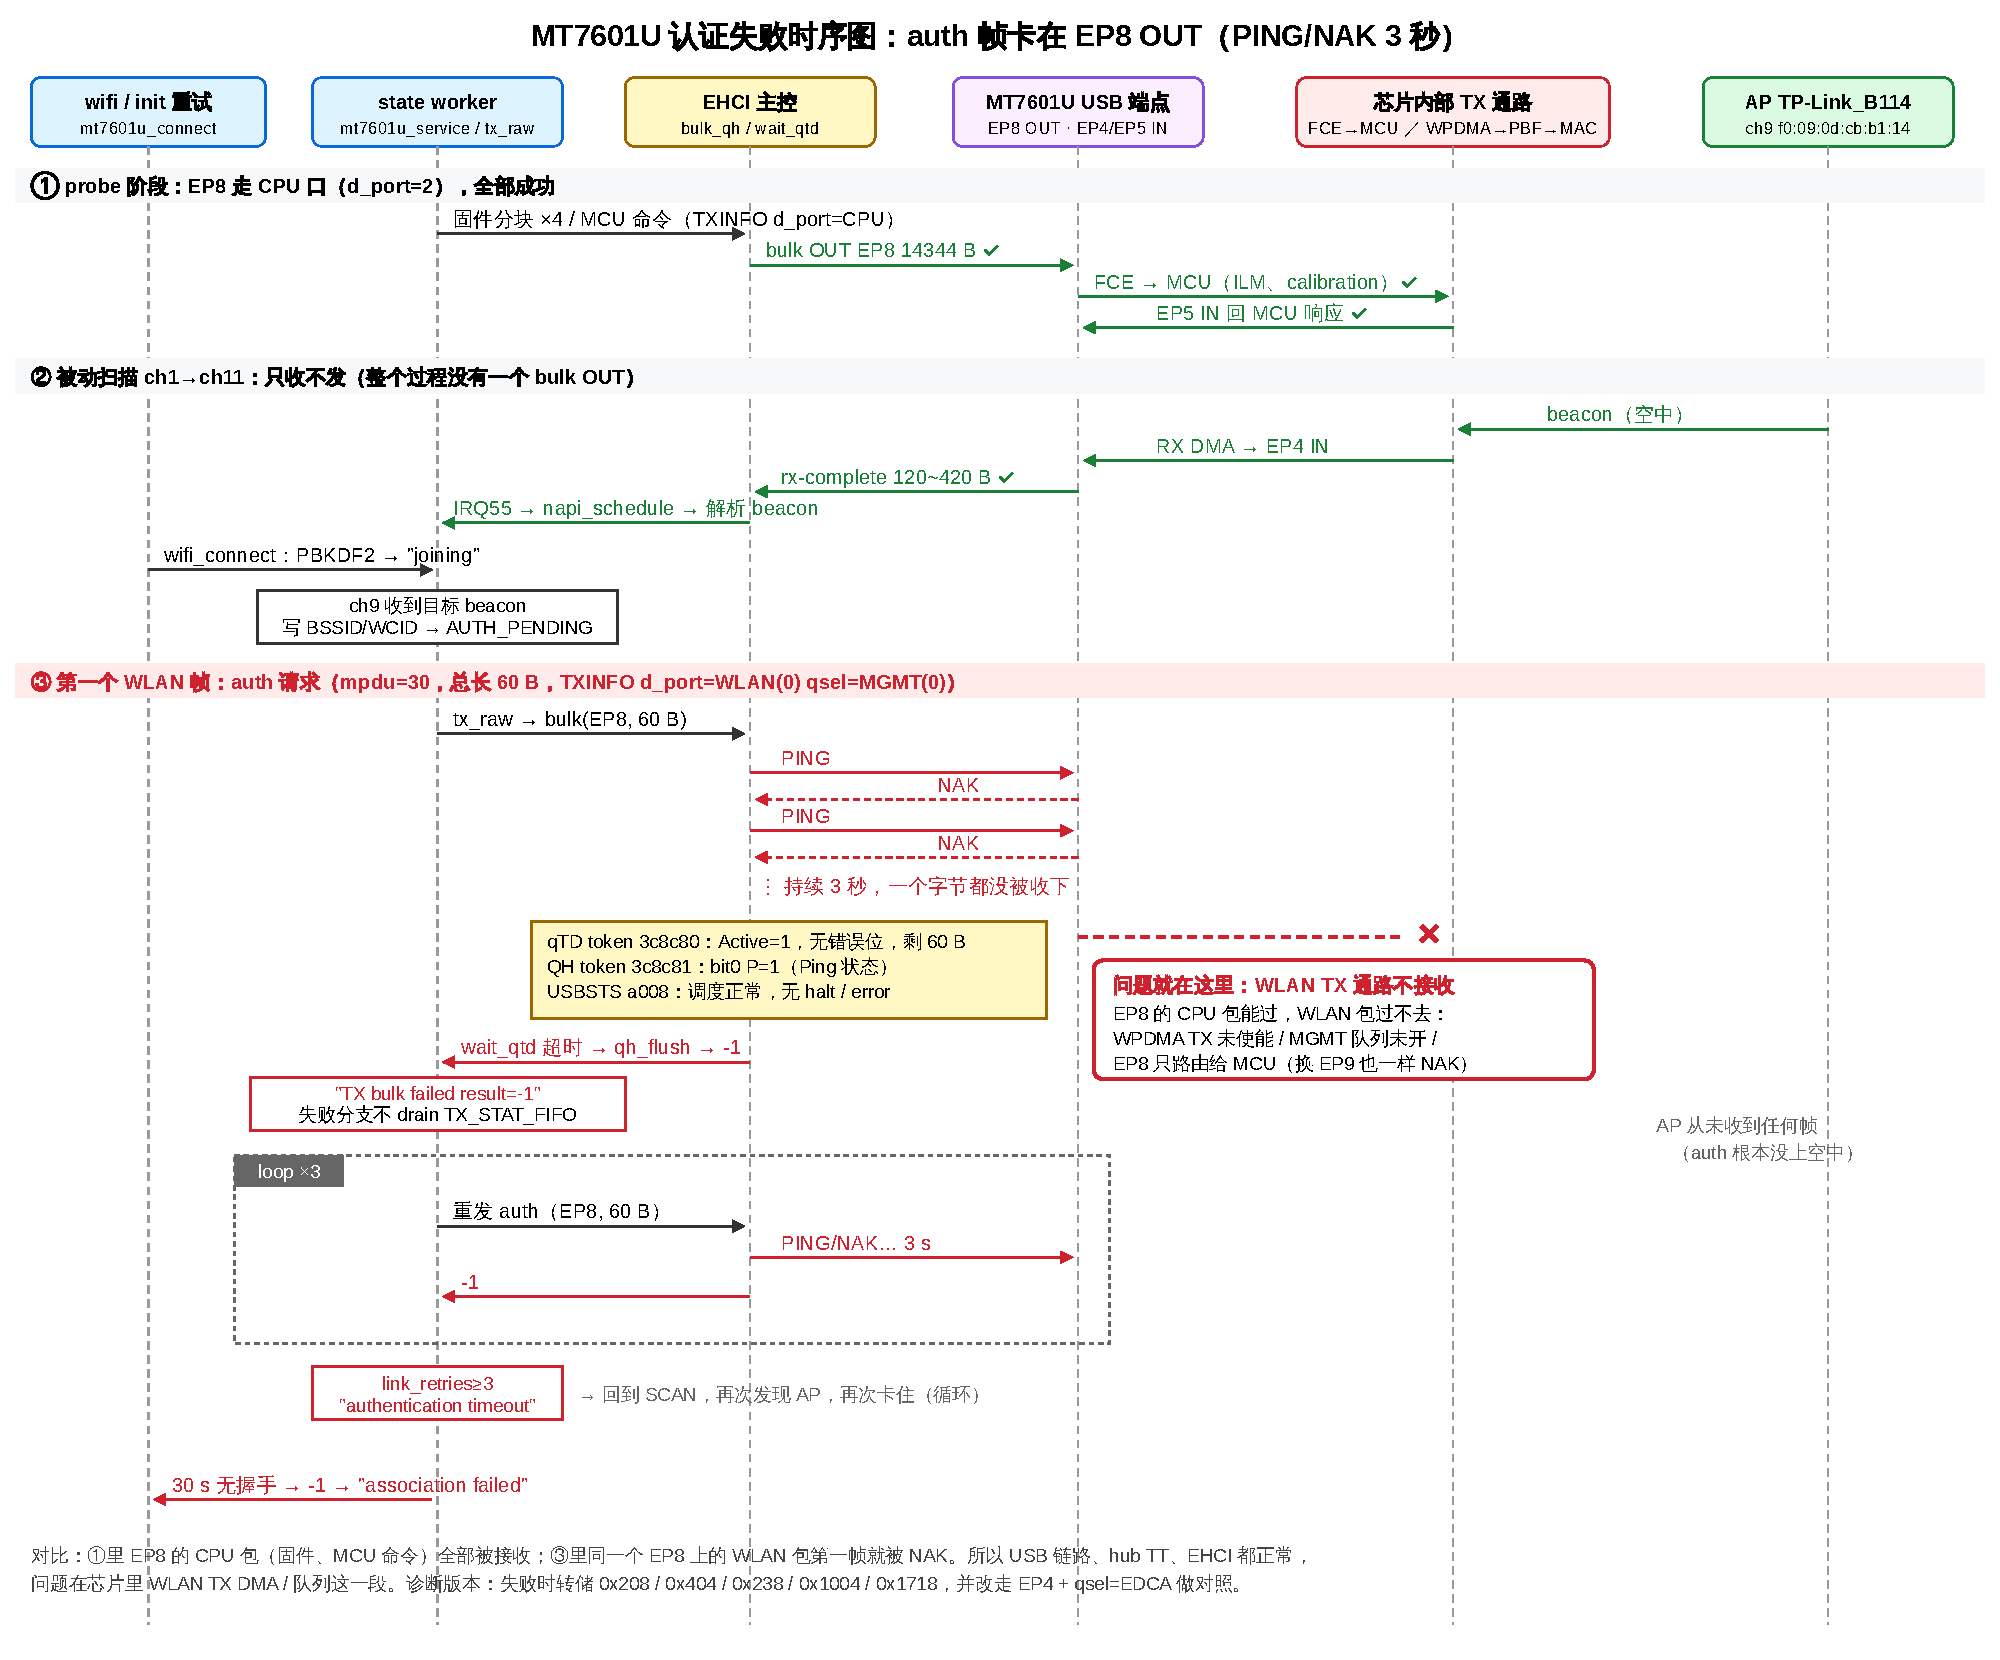
\includegraphics[width=\textwidth]{figures/mt7601u-tx-stall-seq.pdf}
\caption{时序图：auth 帧卡在 EP8 OUT（PING/NAK 3 秒）}\label{dbg:stall}
\end{figure}

现象：\fn{bulk ep8 out 60 bytes failed token=-1}，qTD 一直 Active，主机收到 PING/NAK 3 s 后超时，
\fn{authentication timeout}。加上 \fn{MT7601U\_WCID\_CLEAR=0}（跳过 3977211 引入的 WCID/key 表清零）后，
同样的 EP8/MGMT 路径连续两次上板都正常发完。

\subsubsection{第二阶段：固定 ch9 后 auth 成功、关联无效}

\begin{figure}[H]
\centering
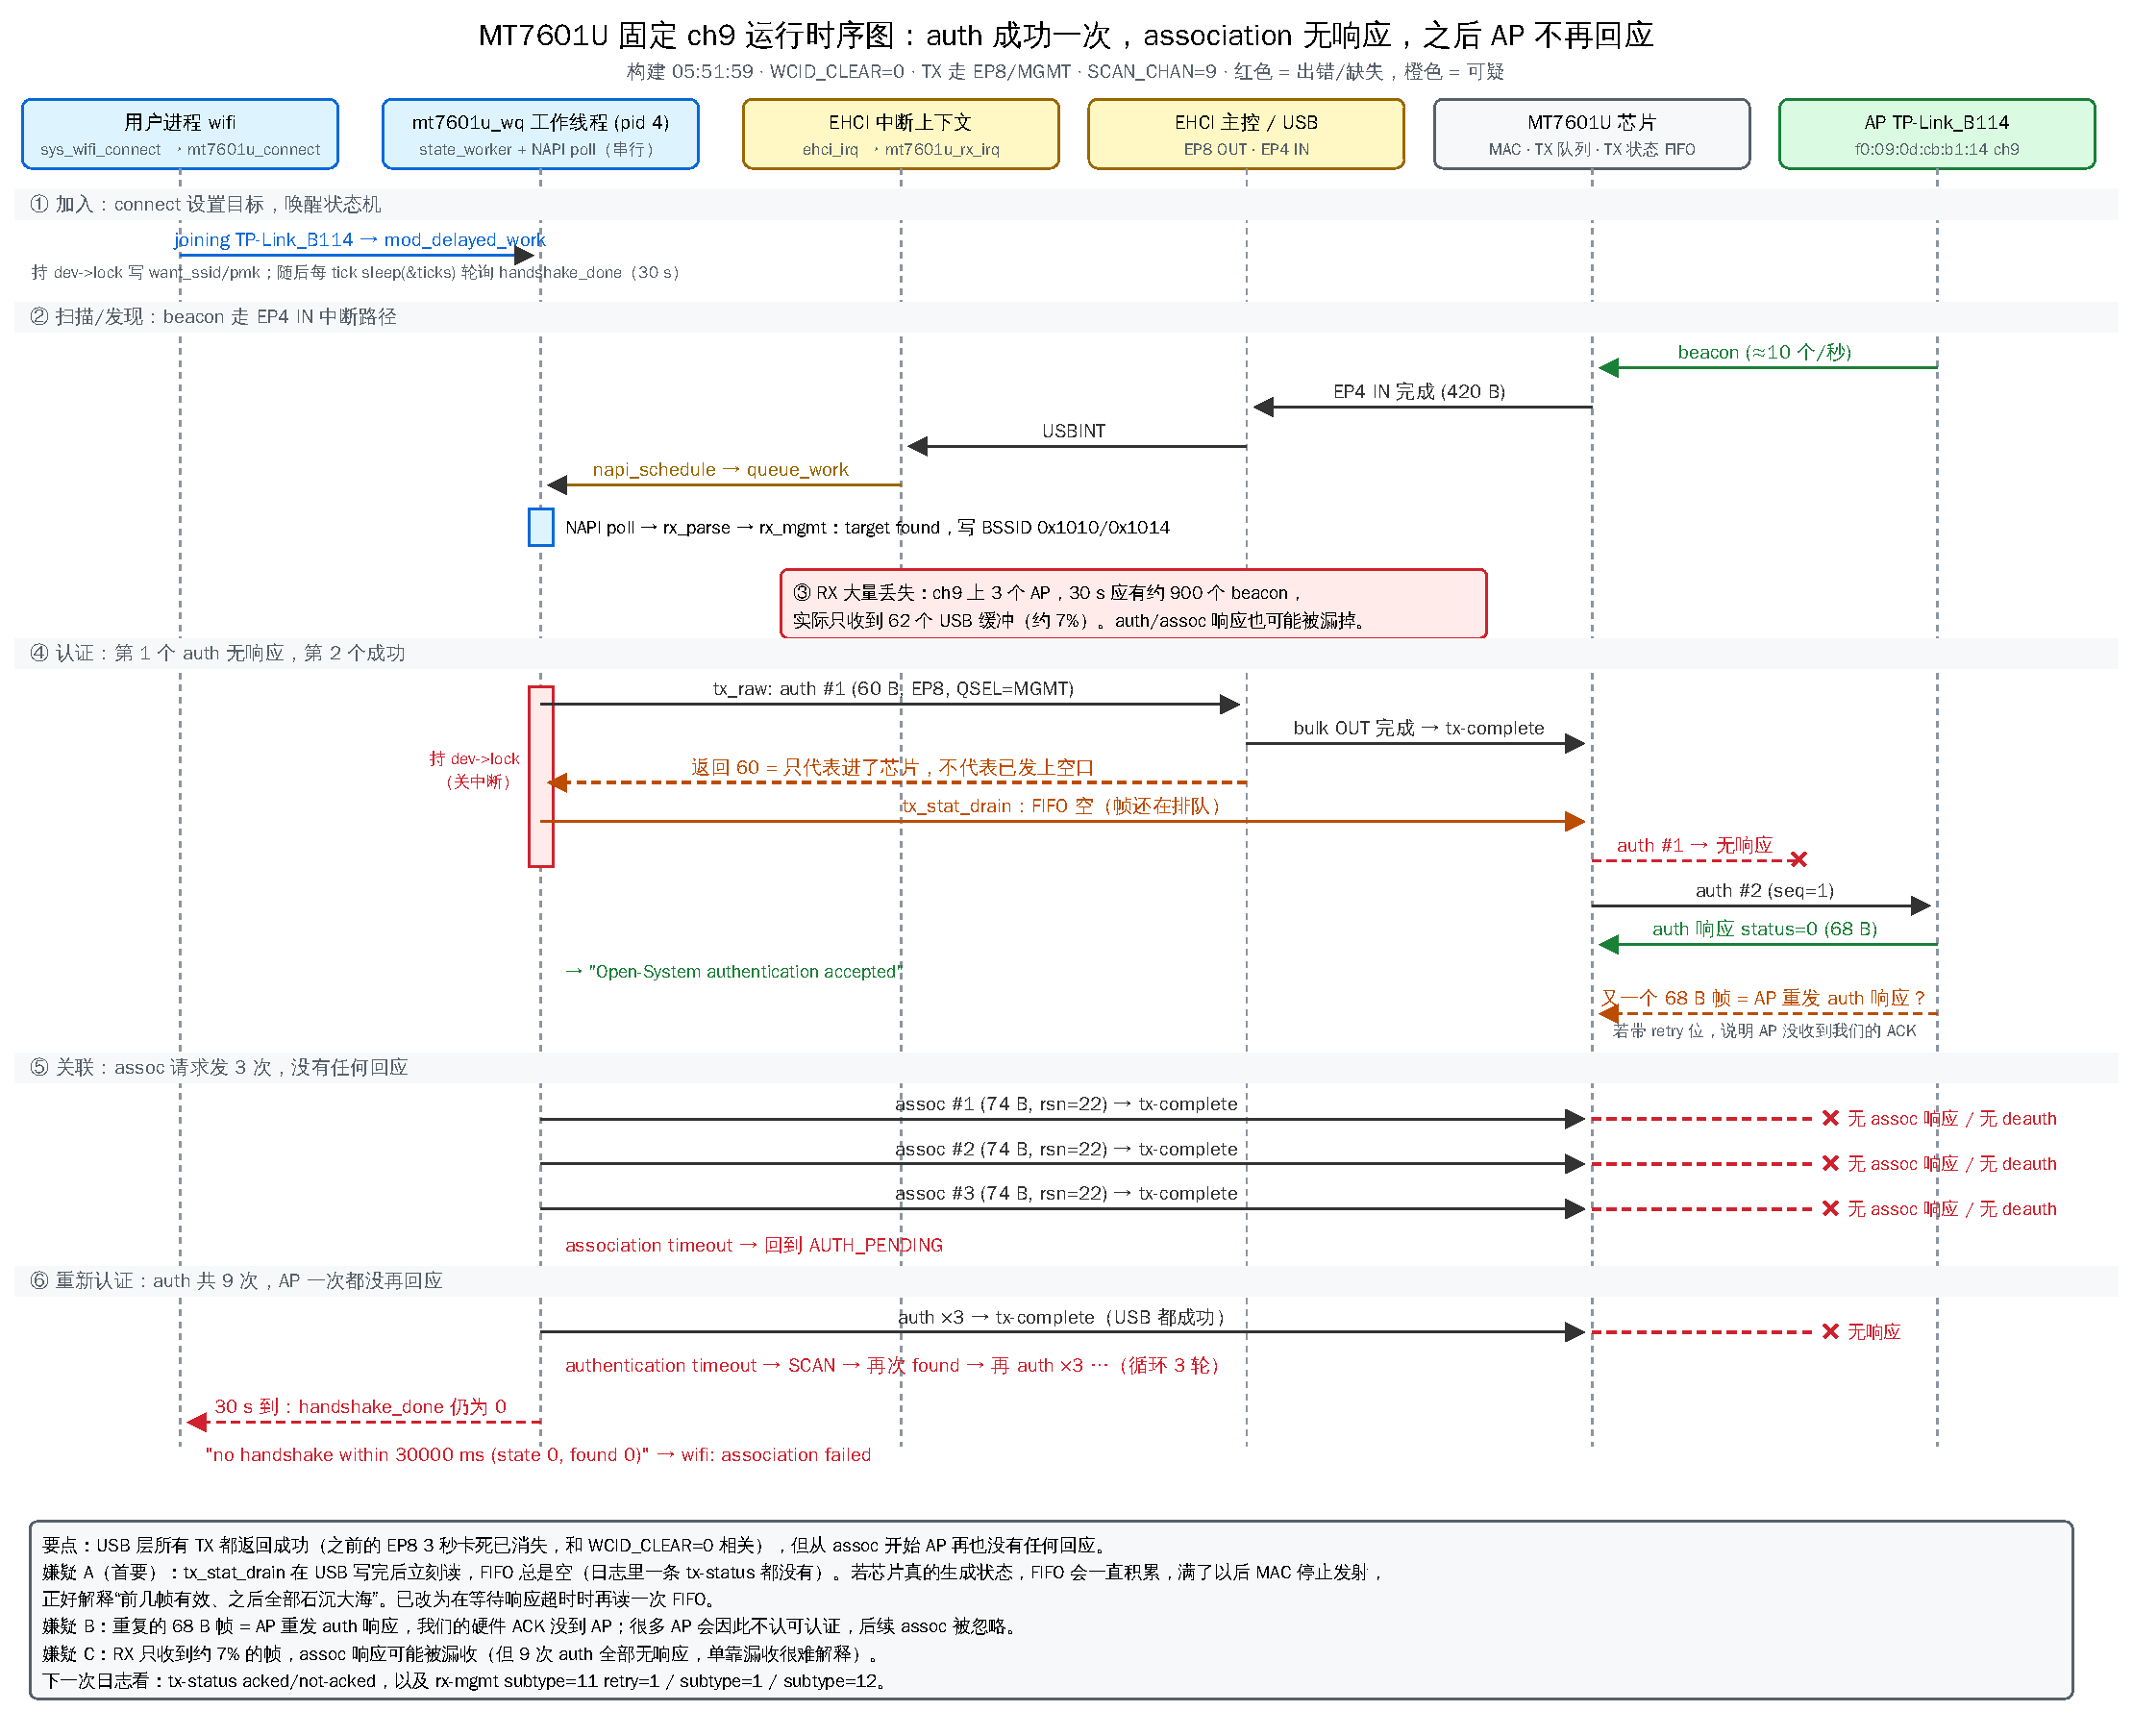
\includegraphics[width=\textwidth]{figures/mt7601u-ch9-assoc-seq.pdf}
\caption{时序图：固定 ch9，auth 成功一次，association 之后 AP 不再回应}\label{dbg:assoc}
\end{figure}

关键日志：

\begin{dbglog}
wifi-data: rx-mgmt subtype=11 retry=1 seq=95  from=cb:b1:14 len=30 body=0 2 0
mt7601u: Open-System authentication accepted
mt7601u: association request sent rsn=22 bytes
wifi-data: rx-mgmt subtype=11 retry=1 seq=103 ...      <- auth 响应仍在重发
wifi-data: rx-mgmt subtype=1  retry=1 seq=104 ... body=1c11 0 c00a
mt7601u: 802.11 associated aid=10; WPA2 handshake pending
wifi-data: rx-mgmt subtype=1  retry=0 seq=2 ...        <- assoc 响应 10 多个，序号各不相同
...
mt7601u: WPA2 M1 timeout; reassociating
\end{dbglog}

解读：AP 的 auth/assoc 响应全部带 retry=1 反复重发，说明 AP 收不到我们的 ACK；我们只发了 1 个 assoc 请求，
却收到十几个序号不同的 assoc 响应，说明我们的 MAC 也收不到 AP 的 ACK，按 \fn{TX\_RTY\_CFG}(0x134c)
自动重发了 assoc 请求。AP 只有在 assoc 响应被 ACK 后才发 EAPOL M1，所以 M1 永远不来。

\subsubsection{全部问题与处理}

\begin{longtable}{p{5mm}p{30mm}p{45mm}p{48mm}p{18mm}}
\toprule
\# & 现象 & 根因 & 处理 & 状态 \\ \midrule \endhead
1 & 开机立即 \fn{association failed} & init 首次调用时 USB 未枚举，驱动未注册 & init 自动重试 10 次 & 正常行为 \\
2 & connect 的 30 s 耗在 probe 上 & probe 一开始就置 \fn{used}，connect 立刻计时 & 新增 \fn{ready}，probe 结束才置 1；connect 先等 ready（$\le$60 s） & 已修，已验证 \\
3 & \fn{napi\_schedule} 日志刷屏 & 每个中断打印一行 & 只打前 4 次，之后每 256 次一行 & 已修 \\
4 & \fn{USB\_WIFI\_TRACE=1} 未打印全部 & level 1 只开 data/config；wifi-reg/frame 要 level 2 & 说明开关含义；改开关自动重编译 & 非 bug \\
5 & auth 卡在 EP8 OUT（PING/NAK 3 s） & 与 3977211 的 WCID/key 表清零相关 & \fn{MT7601U\_WCID\_CLEAR=0} 绕过；\fn{MT7601U\_TX\_EDCA\_EP4} 试验开关（不需要） & 绕过，默认值待定 \\
6 & 跳过清零仍打印 "tables cleared" & printf 在 \fn{\#if} 之外 & 打印随开关变化 & 已修 \\
7 & 扫描找不到 TP-Link\_B114 & 每信道 500 ms + RX 严重丢帧（AP 实际在 ch9） & \fn{MT7601U\_SCAN\_CHAN=9} 固定信道，同信道不再重复调谐 & 诊断手段 \\
8 & 怀疑 TX 状态 FIFO 积满停发 & — & 超时时读 FIFO：没有任何状态 & 已排除 \\
9 & 关联后 \fn{WPA2 M1 timeout} & 802.11 ACK 双向丢失：\fn{MAC\_ADDR\_DW1} 的 UNICAST\_TO\_ME 掩码为 0，芯片不自动回 ACK（曾怀疑频偏/供电，\fn{rx-phy} 已排除频偏） & \fn{MAC\_ADDR\_DW1} 补 UNICAST\_TO\_ME 掩码 0xff$\ll$16（同 Linux）；另加 \fn{rx-mgmt}、\fn{rx-phy} 诊断 & 已修，上板拿到 DHCP \\
10 & \fn{rx-drop icv=1 fc=4208} & 其他终端的加密广播数据，无密钥 & 忽略 & 正常 \\
11 & 锁 & \fn{dev->lock} 跨 USB 传输持有（关中断）；自旋锁内取睡眠锁 & 计划把 USB I/O 移出自旋锁或改为睡眠锁 & 未改 \\
\bottomrule
\end{longtable}

复现命令：

\begin{dbgcode}
make tiny210-sdimg USB_WIFI_TRACE=1 USB_XFER_TRACE=0 \
     MT7601U_TX_EDCA_EP4=0 MT7601U_WCID_CLEAR=0 MT7601U_SCAN_CHAN=9
\end{dbgcode}


\subsubsection{结果：UNICAST\_TO\_ME 掩码修复 ACK}

\fn{MAC\_ADDR\_DW1} 原来只写 MAC 的最后两字节，bits 23:16（UNICAST\_TO\_ME 掩码）为 0；改为与 Linux
\fn{mt7601u\_set\_macaddr} 相同的 0xff 后（日志 \fn{MAC=ff9495:1480de90}），同样的固定 ch9 运行：

\begin{dbglog}
mt7601u: 802.11 associated aid=10; WPA2 handshake pending
mt7601u: received WPA2 EAPOL M1 key-info=8a
mt7601u: sent WPA2 EAPOL M2 replay=0001
mt7601u: keys installed: PTK wcid=1 attr=9, GTK idx=1 skey-mode=40
mt7601u: WPA2 four-way handshake complete
wifi: associated
dhcp: dev=wlan0 address=192.168.0.219 gateway=192.168.0.1 dns=192.168.0.1
arp: dev=wlan0 gateway 192.168.0.1 is f0:9:d:cb:b1:14
\end{dbglog}

\begin{itemize}[leftmargin=2em]
\item \fn{rx-phy} 显示 \fn{freq\_off=15} 稳定、SNR 55--76，频偏校准不是问题。
\item 逐帧 RX 日志降到 level 2：level 1 下 115200 波特率串口本身让 EP4 环一直满（\fn{done=4 completed=0}）。
\item 遗留：M4 发了 3 次（AP 重发 M3），DHCP 首次重试时收到 \fn{deauth reason=6}，驱动自动重连后成功。
\item 待确认：默认参数（\fn{WCID\_CLEAR=1}、自动扫描）下是否同样能连上。
\end{itemize}


\subsubsection{成功连接的完整通信过程（对应通信图 0--8）}\label{dbg:steps}

下面每一步对应图~\ref{dbg:comm} 中的编号，日志全部取自 2026-11-16 06:23 构建（固定 ch9、\fn{WCID\_CLEAR=0}、UNICAST\_TO\_ME 已修）的成功运行。

\begin{dbgcode}
ehci-enum(probe) -0-> IRQ ready
wifi(connect) -1-> work A -2-> EHCI -EP8-> chip -6-> AP
AP -7-> chip -EP4-> EHCI -3-> IRQ -4-> work B -5-> rx_parse/rx_mgmt/rx_data
work A/B -8-> wifi(connect returns 0) -> DHCP -> ARP
\end{dbgcode}

\paragraph*{0. probe 完成，IRQ 交给 NAPI}
\begin{itemize}[leftmargin=2em,itemsep=1pt]
\item \textbf{方向}：ehci-enum kthread → mt7601u 驱动 → EHCI IRQ
\item \textbf{锁}：enum\_lock · dev->lock · xfer\_lock
\item \textbf{过程}：ehci\_enum\_thread → usb-core match → mt7601u\_probe：下载固件(EP8)、eFuse/MAC/BBP/RF 表(EP0)、挂 4 个 EP4 接收缓冲；最后 \_\_sync\_synchronize(); ready=1。此后 EHCI 的 USBINT 才转给 napi\_schedule。
\end{itemize}
\begin{dbglog}
wifi-config: basic init end USB_DMA_CFG=e08020 MAC=ff9495:1480de90   <- UNICAST_TO_ME=0xff
mt7601u: EP4 receive uses USB host IRQ with 4 buffers
mt7601u: transport and MCU ready; SoftMAC initialization pending
usb-core: probe end driver=mt7601u device=148f:7601 result=0
wifi-data: EHCI IRQ -> napi_schedule (#1)
\end{dbglog}

\paragraph*{1. connect 设置目标、唤醒状态机}
\begin{itemize}[leftmargin=2em,itemsep=1pt]
\item \textbf{方向}：用户进程 wifi → mt7601u\_wq（work A）
\item \textbf{锁}：dev->lock · wq->lock · delayed\_lock · tickslock
\item \textbf{过程}：/bin/wifi → sys\_wifi\_connect → mt7601u\_connect：等 ready → PBKDF2 算 PMK → 持 dev->lock 写 want\_ssid/pmk、link\_state=SCAN → mod\_delayed\_work(state\_work) → 每 tick sleep(\&ticks) 轮询 handshake\_done（30 s）。
\end{itemize}
\begin{dbglog}
wifi: connecting to TP-Link_B114
mt7601u: joining TP-Link_B114
\end{dbglog}

\paragraph*{2. work A 发起 USB 传输（调谐 + 发管理帧）}
\begin{itemize}[leftmargin=2em,itemsep=1pt]
\item \textbf{方向}：mt7601u\_wq work A → EHCI 主控（EP0 / EP8 OUT）
\item \textbf{锁}：dev->lock（关中断）· xfer\_lock（睡眠锁）· ehci\_lock
\item \textbf{过程}：state\_worker → mt7601u\_service(0,1)：set\_channel 用 EP0 写 RF bank0 R17–20、BBP62–64、VCO 校准；send\_auth/assoc → tx\_raw：TXINFO(QSEL=MGMT)+TXWI(20 B)+802.11 帧 → ehci\_usb\_bulk(EP8) → wait\_qtd 直到 qTD 完成。
\end{itemize}
\begin{dbglog}
wifi-config: set-channel begin old=1 new=9 gain=55
wifi-config: set-channel end channel=9
mt7601u: target TP-Link_B114 found bssid=f0:9:d:cb:b1:14 channel=9 WPA2 (radio on 9)
mt7601u: WLAN TX path EP8 qsel=MGMT
wifi-data: tx-complete EP8 usb-bytes=60 mpdu=30
mt7601u: authentication request sent
\end{dbglog}

\paragraph*{3. EP4 收到帧，主控产生 USBINT}
\begin{itemize}[leftmargin=2em,itemsep=1pt]
\item \textbf{方向}：EHCI 主控 → 中断上下文（IRQ 55）
\item \textbf{锁}：—（硬件）
\item \textbf{过程}：芯片把收到的 802.11 帧（RXINFO+RXWI+帧）经 EP4 IN 送进已挂好的 16 KB 缓冲，qTD 完成 → USBSTS.USBINT → VIC → ehci\_irq。日志按前 4 次、之后每 256 次打印一次。
\end{itemize}
\begin{dbglog}
wifi-data: EHCI IRQ -> napi_schedule (#2)
wifi-data: EHCI IRQ -> napi_schedule (#256)
wifi-data: EHCI IRQ -> napi_schedule (#512)
\end{dbglog}

\paragraph*{4. 中断里只调度 NAPI}
\begin{itemize}[leftmargin=2em,itemsep=1pt]
\item \textbf{方向}：中断上下文 → mt7601u\_wq（work B）
\item \textbf{锁}：napi->lock · wq->lock
\item \textbf{过程}：ehci\_irq → mt7601u\_rx\_irq（used \&\& ready）→ napi\_schedule：置 scheduled（已在跑则置 missed）→ queue\_work(napi->work)。中断里不做任何 USB 传输。
\end{itemize}
\begin{dbglog}
（每次中断一次；与第 3 步共用同一行日志）
\end{dbglog}

\paragraph*{5. work B 取帧、解析、重挂缓冲}
\begin{itemize}[leftmargin=2em,itemsep=1pt]
\item \textbf{方向}：EHCI 主控 → mt7601u\_wq work B
\item \textbf{锁}：dev->lock · ehci\_lock
\item \textbf{过程}：napi\_workfn → poll → mt7601u\_service(1,0) → bulk\_rx\_complete(EP4) → rx\_parse（按 dma\_len 拆聚合）→ rx\_mgmt（beacon/auth/assoc/deauth）或 rx\_data（EAPOL、IP）→ bulk\_rx\_arm 重挂。budget=4，满 4 个则再调度。
\end{itemize}
\begin{dbglog}
wifi-data: rx-frame #20 fc=80 from=cb:b1:14 seq=1635 len=383      <- beacon，seq 递增=真实流量
mt7601u: AP ssid=TP-Link_B114 bssid=f0:9:d:cb:b1:14 channel=9 WPA2
wifi-data: rx-phy from-ap subtype=8 snr=62 gain=d2 lna=3 vga=18 freq_off=15 rate=0
wifi-data: rx-decapsulate ethertype=806 ethernet-bytes=42 to-me=1
wifi-data: deliver ethernet bytes=42 -> net_rx_dev(wlan0)
\end{dbglog}

\paragraph*{6. 板子 → AP（空口发送）}
\begin{itemize}[leftmargin=2em,itemsep=1pt]
\item \textbf{方向}：MT7601U 芯片 → AP TP-Link\_B114
\item \textbf{锁}：—（芯片 MAC，硬件重试 TX\_RTY\_CFG）
\item \textbf{过程}：EP8 收到的帧进入 MAC 管理队列，1 Mbit/s CCK 发出，等待 AP 的 ACK；收不到会自动重发。依次：auth(seq=1)、assoc(SSID+8 速率+RSN 22 B)、EAPOL M2/M4（work A/B），连上后 DHCP/ARP 走 mt7601u\_net\_xmit。
\end{itemize}
\begin{dbglog}
mt7601u: authentication request sent
wifi-data: tx-complete EP8 usb-bytes=104 mpdu=74
mt7601u: association request sent rsn=22 bytes
wifi-data: tx-complete EP8 usb-bytes=184 mpdu=153
mt7601u: sent WPA2 EAPOL M2 replay=0001
mt7601u: sent WPA2 EAPOL M4
wifi-data: net-xmit ethertype=800 len=342 dst=ff:ff:ff:ff:ff:ff result=0   <- DHCP discover
\end{dbglog}

\paragraph*{7. AP → 板子（响应、握手、数据）}
\begin{itemize}[leftmargin=2em,itemsep=1pt]
\item \textbf{方向}：AP TP-Link\_B114 → MT7601U 芯片（再经第 3–5 步上交）
\item \textbf{锁}：—（芯片对发给自己的帧自动回 ACK）
\item \textbf{过程}：AP 的 auth/assoc 响应、EAPOL M1/M3、DHCP、ARP 都要被我们 ACK。UNICAST\_TO\_ME 掩码修好后，assoc 响应只重发 1 次，M1 随即到来；PTK/GTK 写入 WCID 1 / 共享密钥表，之后数据帧由硬件解密。
\end{itemize}
\begin{dbglog}
wifi-data: rx-mgmt subtype=11 retry=1 seq=8 from=cb:b1:14 len=30 body=0 2 0
mt7601u: Open-System authentication accepted
wifi-data: rx-mgmt subtype=1 retry=1 seq=9 from=cb:b1:14 len=107 body=1c11 0 c00a
mt7601u: 802.11 associated aid=10; WPA2 handshake pending
mt7601u: received WPA2 EAPOL M1 key-info=8a
mt7601u: keys installed: PTK wcid=1 attr=9, GTK idx=1 skey-mode=40
dhcp: dev=wlan0 address=192.168.0.219 gateway=192.168.0.1 dns=192.168.0.1
arp: dev=wlan0 gateway 192.168.0.1 is f0:9:d:cb:b1:14
\end{dbglog}

\paragraph*{8. 握手完成，connect 返回}
\begin{itemize}[leftmargin=2em,itemsep=1pt]
\item \textbf{方向}：mt7601u\_wq → 用户进程 wifi
\item \textbf{锁}：dev->lock · tickslock
\item \textbf{过程}：M4 发出后 handshake\_done=1、注册 wlan0；connect 的轮询循环看到 handshake\_done 返回 0，/bin/wifi 打印 associated，init 接着跑 DHCP。之后 AP 发 deauth reason=6，驱动自动重连并再次完成握手。
\end{itemize}
\begin{dbglog}
mt7601u: WPA2 four-way handshake complete
mt7601u: wlan0 registered mac=90:de:80:14:95:94
wifi: associated
mt7601u: deauthentication from AP reason=6 (link_state=5 handshake=1)
mt7601u: reconnecting
\end{dbglog}

\paragraph*{小结}

\begin{longtable}{p{12mm}p{30mm}p{25mm}p{22mm}p{62mm}}
\toprule
阶段 & 帧（方向） & 发送路径 & 接收路径 & 关键日志 \\ \midrule \endhead
扫描 & beacon（AP→板） & — & 3→4→5 & \fn{rx-frame ... from=cb:b1:14} \\
认证 & auth 请求/响应 & 2→6 & 7→3→4→5 & \fn{Open-System authentication accepted} \\
关联 & assoc 请求/响应 & 2→6 & 7→3→4→5 & \fn{associated aid=10} \\
WPA2 & M1/M3（AP→板）、M2/M4（板→AP） & 5 中调 \fn{tx\_raw} → 6 & 7→3→4→5 & \fn{received M1}、\fn{keys installed}、\fn{sent M4} \\
完成 & — & — & — & \fn{four-way handshake complete}、\fn{wifi: associated}（8） \\
DHCP/ARP & IP/ARP 数据帧 & \fn{net\_xmit} → EP8 → 6 & 7→3→4→5 & \fn{address=192.168.0.219}、\fn{gateway ... is f0:9:d:cb:b1:14} \\
\bottomrule
\end{longtable}

每一个从 AP 来的单播帧（auth/assoc 响应、M1/M3、DHCP、ARP）都需要芯片在 SIFS 内自动回 ACK，这一步依赖 \fn{MAC\_ADDR\_DW1} 的 UNICAST\_TO\_ME 掩码；掩码为 0 时第 7 步的帧虽能收到，AP 却收不到 ACK，会不停重发并且不发 M1。

\subsubsection{每一步的函数、USB 传输方式与数据格式}\label{dbg:steps-detail}

与图~\ref{dbg:comm} 卡片中的“函数 / USB 传输 / 数据格式”三行一致，均按源码（\fn{mt7601u.c}、\fn{ehci-hcd.c}）核对。

\paragraph*{0. probe 完成，IRQ 交给 NAPI}
\begin{itemize}[leftmargin=2em,itemsep=1pt]
\item \textbf{函数}：ehci\_enum\_thread → enumerate → usb-core match → mt7601u\_probe → mt7601u\_load\_firmware/mt7601u\_dma\_fw\_chunk → mt7601u\_read\_eeprom/mt7601u\_efuse\_read\_block → mt7601u\_basic\_hw\_init → mt7601u\_mcu\_command → mt7601u\_full\_hw\_init(mt7601u\_bbp\_write / mt7601u\_rf\_write) → mt7601u\_set\_channel → bulk\_rx\_arm×4
\item \textbf{USB 传输}：EP0 控制（ehci\_usb\_control → control\_qh：Setup+Data+Status 三个 qTD，wait\_qtd 同步）；EP8 bulk OUT 固件/MCU 命令（ehci\_usb\_bulk → bulk\_qh，同步）；EP5 bulk IN MCU 应答（同步）；EP4 bulk IN ×4 异步预挂（ehci\_usb\_bulk\_rx\_arm，qTD 带 IOC）
\item \textbf{数据格式}：读 32 位 Setup C0 07 0000 reg 0004 → 4 B 小端；写 32 位 40 02 lo reg / 40 02 hi reg+2（无数据阶段）；BBP\_CSR = val\textbar{}reg\textless{}\textless{}8\textbar{}WRITE\textbar{}BUSY；RF\_CSR = val\textbar{}reg\textless{}\textless{}8\textbar{}bank\textless{}\textless{}14\textbar{}WRITE\textbar{}KICK；固件：FCE(0x42) 写 DMA\_ADDR/DMA\_LEN，再 EP8 [TXINFO (2\textless{}\textless{}27)\textbar{}len][块][4B 0]；MCU：[TXINFO 1\textless{}\textless{}30\textbar{}2\textless{}\textless{}27\textbar{}cmd\textless{}\textless{}20\textbar{}seq\textless{}\textless{}16\textbar{}len][payload][4B 0]，EP5 回 16 B（如 4a010008）
\end{itemize}

\paragraph*{1. connect 设置目标、唤醒状态机}
\begin{itemize}[leftmargin=2em,itemsep=1pt]
\item \textbf{函数}：/bin/wifi → sys\_wifi\_connect → mt7601u\_connect → wpa\_pbkdf2 → mod\_delayed\_work(state\_work) → 循环 sleep(\&ticks)
\item \textbf{USB 传输}：无
\item \textbf{数据格式}：内存：want\_ssid、pmk[32]、link\_state=SCAN
\end{itemize}

\paragraph*{2. work A 发起 USB 传输}
\begin{itemize}[leftmargin=2em,itemsep=1pt]
\item \textbf{函数}：mt7601u\_state\_worker → mt7601u\_service(0,1) → mt7601u\_set\_channel ｜ mt7601u\_send\_auth/send\_assoc → mt7601u\_build\_mgmt\_header → mt7601u\_tx\_mgmt → mt7601u\_tx\_raw → ehci\_usb\_bulk(EP8)
\item \textbf{USB 传输}：调谐：EP0 控制（RF bank0 R17–20、BBP62–64、VCO R4/R5）；发帧：EP8 bulk OUT 同步，高速 OUT 由主控 PING/NAK 流控，3 s 超时
\item \textbf{数据格式}：[TXINFO 4B][TXWI 20B][802.11 MPDU][补齐 4B][4B 0]（位域见图末）；TXWI rate\_ctl=0（CCK 1M）ack\_ctl=1 wcid=0xff len\_ctl=MPDU 长；auth MPDU 30 B → USB 60 B，assoc 74 B → 104 B
\end{itemize}

\paragraph*{3. EP4 完成，主控产生 USBINT}
\begin{itemize}[leftmargin=2em,itemsep=1pt]
\item \textbf{函数}：主控硬件完成 qTD → USBSTS.USBINT → VIC → ehci\_irq
\item \textbf{USB 传输}：EP4 bulk IN：主控异步调度自动轮询设备，CPU 不参与
\item \textbf{数据格式}：USBSTS 写 1 清零（W1C）；EP4 数据落在预挂的 16 KB 缓冲（格式见第 5 步）
\end{itemize}

\paragraph*{4. 中断里只调度 NAPI}
\begin{itemize}[leftmargin=2em,itemsep=1pt]
\item \textbf{函数}：ehci\_irq → mt7601u\_rx\_irq（used \&\& ready）→ napi\_schedule → queue\_work(napi->work)
\item \textbf{USB 传输}：无
\item \textbf{数据格式}：只改 napi->scheduled / missed 标志
\end{itemize}

\paragraph*{5. work B 取帧、解析、重挂缓冲}
\begin{itemize}[leftmargin=2em,itemsep=1pt]
\item \textbf{函数}：napi\_workfn → mt7601u\_napi\_poll → mt7601u\_service(1,0) → ehci\_usb\_bulk\_rx\_complete → mt7601u\_rx\_parse → mt7601u\_rx\_mgmt ｜ mt7601u\_rx\_data → mt7601u\_rx\_eapol / net\_rx\_dev → ehci\_usb\_bulk\_rx\_arm
\item \textbf{USB 传输}：从 QH 摘下已完成 qTD（TOK\_ACTIVE=0），同一块 16 KB 缓冲再挂回
\item \textbf{数据格式}：一个 USB 缓冲可聚合多帧，每段 [DMA 头 4B dma\_len][RXWI 28B][MPDU][补齐][4B 尾]，段长 = dma\_len+8；RXINFO bit8 CRC、9 ICV、10 MIC、14 L2PAD、16 DECRYPT；RXWI 字节 16 SNR、18 增益、19 freq\_off
\end{itemize}

\paragraph*{6. 板子 → AP（空口发送）}
\begin{itemize}[leftmargin=2em,itemsep=1pt]
\item \textbf{函数}：管理帧同第 2 步；EAPOL：mt7601u\_rx\_eapol → mt7601u\_send\_m2/send\_m4 → mt7601u\_send\_llc → mt7601u\_tx\_raw；数据：mt7601u\_net\_xmit → mt7601u\_send\_llc → mt7601u\_tx\_raw
\item \textbf{USB 传输}：EP8 bulk OUT 同步；芯片 MAC 以 CCK 1 Mbit/s 发上空口，无 ACK 按 TX\_RTY\_CFG 重发
\item \textbf{数据格式}：auth fc=00b0 体 0 1 0；assoc fc=0000 体 能力+listen 10+SSID IE+8 速率+RSN IE 22B；EAPOL fc=0108（Data+ToDS）+ LLC aa aa 03 00 00 00 88 8e + EAPOL-Key（M2 153 B，WIV=1 不加密）；DHCP/ARP fc=4108（+Protected，WCID 1 的 PTK 硬件 CCMP），LLC 0800/0806
\end{itemize}

\paragraph*{7. AP → 板子（响应、握手、数据）}
\begin{itemize}[leftmargin=2em,itemsep=1pt]
\item \textbf{函数}：芯片自动回 ACK → 第 3→4→5 步 → mt7601u\_rx\_mgmt（auth/assoc 响应）｜ mt7601u\_rx\_data → mt7601u\_rx\_eapol（M1/M3 → mt7601u\_install\_ccmp\_keys：WCID 1 PTK + GTK）｜ net\_rx\_dev（DHCP/ARP）
\item \textbf{USB 传输}：EP4 bulk IN（异步）
\item \textbf{数据格式}：auth 响应 fc=00b0 体 0 2 0；assoc 响应 fc=0010 体 1c11 0 c00a（能力、状态 0、AID=10\textbar{}0xc000）；数据 fc=4208（Data+FromDS+Protected），RXINFO DECRYPT=1，跳过 8 B CCMP 头再解 LLC
\end{itemize}

\paragraph*{8. 握手完成，connect 返回}
\begin{itemize}[leftmargin=2em,itemsep=1pt]
\item \textbf{函数}：mt7601u\_send\_m4 → handshake\_done=1 → 注册 wlan0；mt7601u\_connect 循环看到 handshake\_done → return 0 → sys\_wifi\_connect → /bin/wifi 打印 associated
\item \textbf{USB 传输}：无
\item \textbf{数据格式}：共享变量 dev->handshake\_done
\end{itemize}

\paragraph*{描述符位域}
\begin{dbgcode}
TXINFO (EP8 每包前 4 B)
  31   30   29..27        26..25      24   23..20    19      18..16    15..0
  -    CMD  d_port         QSEL        WIV  cmd(MCU)  802.11  seq(MCU)  长度(TXWI+MPDU 补齐到 4)
            WLAN=0,CPU=2   MGMT=0,EDCA=2

EP8 OUT 一包: [TXINFO 4][TXWI 20: flags2 rate_ctl2 ack1 wcid1 len_ctl2 iv4 eiv4 aid/stream/ctl4][MPDU][补齐][0 x4]
EP4 IN 一段: [DMA 头 4: dma_len][RXWI 28: RXINFO4 ctl4(MPDU 长 b16-27) ... SNR@16 gain@18 freq_off@19][MPDU][补齐][尾 4]
RXINFO: bit8 CRC  bit9 ICV  bit10 MIC  bit14 L2PAD  bit16 DECRYPT
EP0 Setup: [bmRequestType C0读/40写][bRequest 7读/2写/0x42 FCE][wValue 写值 16 位][wIndex 寄存器][wLength 4/0]
\end{dbgcode}


\chapter{USB 主机栈：EHCI 数据传输与中断处理}\label{wa:ch-05b-usb-stack}
\section{USB 各层架构}

\begin{figure}[H]
\centering
\begin{tikzpicture}[font=\small,node distance=5mm]
\node[wbox=wamber,text width=128mm] (drv) {MT7601U 驱动：mt7601u\_read32 / write32 / tx\_raw / service};
\node[wbox=tinyblue,text width=128mm,below=of drv] (ops) {struct usb\_host\_ops：control · bulk · bulk\_rx\_arm · bulk\_rx\_complete};
\node[wbox=tinyblue,minimum width=36mm,below=of ops,xshift=-48mm] (c) {ehci\_usb\_control\\control\_qh\\SETUP/DATA/STATUS};
\node[wbox=tinyblue,minimum width=36mm,below=of ops] (b) {ehci\_usb\_bulk\\bulk\_qh（同步）\\wait\_qtd 1 s/3 s};
\node[wbox=tinyblue,minimum width=36mm,below=of ops,xshift=48mm] (r) {bulk\_rx\_arm\\bulk\_rx\_complete\\EP4 预挂 4 个 qTD};
\node[wbox=tinyblue,text width=128mm,below=of b] (qa) {qh\_append：dummy qTD 追加法（硬件始终看到一致链表）；出错时 async\_stop → qh\_flush（保留 DT）→ async\_start};
\node[wbox=tinyblue,text width=128mm,below=of qa] (ring) {异步调度环：head\_qh → ep0 QH(地址1) → ep0 QH(地址2) → EP4 IN QH → EP8 OUT QH → … → head\_qh};
\node[wbox=tinyred,text width=128mm,below=of ring] (hc) {EHCI 硬件：按 QH 取 qTD，DMA 读写 DDR，产生 IN/OUT/PING 事务，完成后清 Active，IOC → USBINT → IRQ 55};
\node[wbox=tinyred,text width=128mm,below=of hc] (phy) {PHY1 → USB2514 Hub → MT7601U};
\draw[warr] (drv) -- (ops);
\draw[warr] (ops) -- (c); \draw[warr] (ops) -- (b); \draw[warr] (ops) -- (r);
\draw[warr] (c) -- (qa); \draw[warr] (b) -- (qa); \draw[warr] (r) -- (qa);
\draw[warr] (qa) -- (ring); \draw[warr] (ring) -- (hc); \draw[wdarr] (hc) -- (phy);
\end{tikzpicture}
\caption{USB 软件分层}
\end{figure}

\subsection{平台层：PHY 与控制器启动}\label{wa:phy}

\fn{host\_phy\_init()}（参考 Linux \fn{phy-s5pv210-usb2.c}）：\fn{CLK\_GATE\_IP1}(0xE0100464) bit17 打开 USBHOST 时钟；
\fn{USB\_PHY\_CONTROL}(0xE010E80C) bit1 解除 PHY1 隔离；PHY 寄存器块 0xEC100000 中 \fn{UPHYCLK} 选 24 MHz，
\fn{UPHYPWR} 清 bit6/7 使 PHY1 上电，\fn{URSTCON} bit3/4 脉冲复位 PHY1 和 Host link。

\fn{ehci\_start()}：
\begin{enumerate}[leftmargin=2em,itemsep=0pt]
\item \fn{phy\_init()}；CAPLENGTH 得到操作寄存器基址，HCSPARAMS 得到端口数（1）。
\item Samsung 私有寄存器 INSNREG00（burst 使能），\textbf{INSNREG01 = 0x00800080}（OUT/IN 阈值均为 512 字节）。
\item 停止、复位控制器；建立异步环头 QH（H 位，halted overlay，指向自己）。
\item \fn{ASYNCLIST = head\_qh}，\fn{USBINTR = USBINT|ERR}，\fn{USBCMD = RUN|ASE|ITC(1)}，\fn{CONFIGFLAG = 1}；端口上电，等 100 ms。
\end{enumerate}
\begin{lstlisting}[basicstyle=\ttfamily\small\color{tinygreen!70!black},backgroundcolor=\color{tinygreen!4}]
ehci: s5p-ehci at -13e00000, enumeration deferred to ehci-enum
ehci: 1 port(s), running, async schedule on
\end{lstlisting}

\subsection{HCD 层：QH/qTD 与 dummy 追加法}

EHCI 异步调度是一个 QH（每端点一个）组成的环，每个 QH 下挂一串 qTD，每个 qTD 最多描述 5 个 4 KiB 页。

\begin{itemize}[leftmargin=2em,itemsep=0pt]
\item \fn{qh\_create(addr, ep, speed, mps, control, hub, port)}：填 epchar（地址、端点、速度、最大包长）、epcap（Hub 地址/端口），挂入环；初始挂一个不活动的 dummy qTD。
\item \fn{qh\_append(q, first, last)}：把新传输第一个 qTD 的内容拷进当前 dummy，在尾部接新 dummy；先激活后续 qTD，最后才置第一个的 Active。无需停异步调度。
\item \fn{wait\_qtd}：轮询最后一个 qTD 的 Active（IN 1 s，OUT 3 s，OUT 期间设备可 NAK/PING）。
\item \fn{qh\_flush}：超时/出错时丢弃排队的 qTD，QH 重新指向 dummy，\textbf{保留 data toggle}。
\item \fn{ehci\_usb\_bulk\_rx\_arm}：给 EP4 预挂带 IOC 的 IN qTD；\fn{ehci\_usb\_bulk\_rx\_}\allowbreak\fn{complete} 从 \fn{q->head} 取已完成的 qTD。
\item \fn{ehci\_irq}：USBSTS 的 USBINT/ERR 置位时调弱符号 \fn{mt7601u\_rx\_irq()}。
\end{itemize}

\subsection{总线上的包与事务}

USB 总线上被调度的最小单位是\textbf{事务}：主机发 Token 包声明“对哪个设备的哪个端点做什么”，接着是可选的 Data 包，
最后由接收方回 Handshake 包。主机发起一切，设备只能应答。

\begin{figure}[H]
\centering
\begin{tikzpicture}[font=\scriptsize]
\def\pk#1#2#3#4{\node[draw,fill=#4!14,minimum height=8mm,minimum width=#2mm,anchor=west,align=center] at (#1mm,0) {#3};}
\node[anchor=east,font=\small\bfseries] at (-1mm,0) {Token};
\pk{0}{14}{SYNC}{wgray}\pk{14}{24}{PID\\OUT/IN/SETUP/PING}{wamber}\pk{38}{26}{ADDR 7 位\\ENDP 4 位}{tinyblue}\pk{64}{12}{CRC5}{tinygreen}\pk{76}{10}{EOP}{tinyred}
\begin{scope}[yshift=-11mm]
\node[anchor=east,font=\small\bfseries] at (-1mm,0) {Data};
\pk{0}{14}{SYNC}{wgray}\pk{14}{24}{PID\\DATA0/DATA1}{wamber}\pk{38}{50}{负载 0--512 B（高速 bulk）}{tinyblue}\pk{88}{14}{CRC16}{tinygreen}\pk{102}{10}{EOP}{tinyred}
\end{scope}
\begin{scope}[yshift=-22mm]
\node[anchor=east,font=\small\bfseries] at (-1mm,0) {Handshake};
\pk{0}{14}{SYNC}{wgray}\pk{14}{50}{PID：ACK / NAK / NYET / STALL}{wamber}\pk{64}{10}{EOP}{tinyred}
\end{scope}
\end{tikzpicture}
\caption{USB 三种包（PID 本身带反码，所以不需要另加 CRC）}
\end{figure}

\begingroup\small\begin{longtable}{p{18mm}p{22mm}p{90mm}}
\toprule
类别 & PID & 含义与本驱动中的位置 \\ \midrule \endhead
Token & SETUP & 只用于 EP0，开始一次控制传输（枚举、MT7601U 寄存器读写） \\
Token & OUT & 主机写端点：EP0 的数据/状态阶段，EP8 的固件、MCU 命令和 802.11 帧 \\
Token & IN & 主机读端点：EP0 的数据阶段，EP4 接收帧，EP5 MCU 应答 \\
Token & PING & 只用于高速 bulk/控制 OUT：先问端点有没有空间，再发数据。EHCI 在 qTD 的 Ping 状态位里自动处理 \\
Data & DATA0 / DATA1 & 交替使用（data toggle），接收方据此识别重传的重复包。SETUP 恒为 DATA0 \\
Handshake & ACK & 正确收到 \\
Handshake & NAK & 暂时不能收/没有数据。是流控不是错误：EP4 空闲时设备对每个 IN 回 NAK，EHCI 按 QH 的 NAK reload 计数自动重试 \\
Handshake & NYET & 高速 OUT：这个包收下了但下一个可能放不下，主机下一次先 PING \\
Handshake & STALL & 端点出错停住，要软件 \fn{CLEAR\_FEATURE(HALT)}；qTD 上表现为 Halted \\
\bottomrule
\end{longtable}\endgroup

四种传输类型里本驱动用了两种：\textbf{控制传输}（EP0，可靠、双向、有 SETUP 阶段）和 \textbf{bulk 传输}（EP4/5/8，可靠、无时限、只用剩余带宽）。
中断传输只在 Hub 的状态端点上有（xv6 不轮询它，没做热插拔），等时传输没用。

\subsection{EHCI 数据结构：QH 与 qTD}

\begin{figure}[H]
\centering
\begin{tikzpicture}[font=\scriptsize,scale=0.95,transform shape]
\node[wbox=wgray,text width=25mm] (h) at (0,0) {head\_qh\\H=1，halted\\指向自己};
\node[wbox=tinyblue,text width=25mm] (q1) at (3.6,0) {QH 地址1 EP0\\(USB2514)};
\node[wbox=tinyblue,text width=25mm] (q2) at (7.2,0) {QH 地址2 EP0\\(MT7601U)};
\node[wbox=tinyblue,text width=25mm] (q3) at (10.8,0) {QH 地址2\\EP4 IN};
\node[wbox=tinyblue,text width=25mm] (q4) at (14.4,0) {QH 地址2\\EP8 OUT / EP5 IN};
\draw[warr] (h) -- (q1);
\draw[warr] (q1) -- (q2); \draw[warr] (q2) -- (q3); \draw[warr] (q3) -- (q4);
\draw[warr] (q4.north) -- ++(0,0.5) -| node[wlbl,pos=0.25]{horiz（异步环）} (h.north);
\node[wbox=tinygreen,text width=25mm] (t1) at (10.8,-1.8) {qTD 16 KiB\\Active, IOC};
\node[wbox=tinygreen,text width=25mm] (t2) at (10.8,-3.3) {qTD 16 KiB};
\node[wbox=tinygreen,text width=25mm] (t3) at (10.8,-4.8) {qTD 16 KiB};
\node[wbox=tinygreen,text width=25mm] (t4) at (10.8,-6.3) {qTD 16 KiB};
\node[wbox=wgray,text width=25mm] (t5) at (10.8,-7.8) {dummy qTD\\不活动};
\draw[warr] (q3) -- node[wlbl,right]{next} (t1); \draw[warr] (t1) -- (t2); \draw[warr] (t2) -- (t3); \draw[warr] (t3) -- (t4); \draw[warr] (t4) -- (t5);
\node[wbox=tinygreen,text width=25mm] (o1) at (14.4,-1.8) {qTD OUT\\388 B（DHCP）};
\node[wbox=wgray,text width=25mm] (o2) at (14.4,-3.3) {dummy};
\draw[warr] (q4) -- (o1); \draw[warr] (o1) -- (o2);
\node[wbox=tinygreen,text width=25mm] (c1) at (7.2,-1.8) {SETUP 8 B};
\node[wbox=tinygreen,text width=25mm] (c2) at (7.2,-3.3) {DATA IN 4 B};
\node[wbox=tinygreen,text width=25mm] (c3) at (7.2,-4.8) {STATUS OUT 0 B, IOC};
\node[wbox=wgray,text width=25mm] (c4) at (7.2,-6.3) {dummy};
\draw[warr] (q2) -- (c1); \draw[warr] (c1) -- (c2); \draw[warr] (c2) -- (c3); \draw[warr] (c3) -- (c4);
\end{tikzpicture}
\caption{异步调度环：每个端点一个 QH，传输是挂在 QH 下的 qTD 链（图中为一次寄存器读和 EP4 的 4 个接收缓冲）}
\end{figure}

\begingroup\small\begin{longtable}{p{13mm}p{27mm}p{94mm}}
\toprule
QH 字 & 字段 & 本驱动填的值（\fn{qh\_create}） \\ \midrule \endhead
0 & horiz & 下一个 QH 的物理地址 | Typ=QH(bit1)。新 QH 插在 head\_qh 后面，一次对齐写完成发布 \\
1 & epchar & [6:0] 设备地址；[11:8] 端点号；[13:12] 速度（2=高速）；[14] DTC（控制端点=1：toggle 取自 qTD）；[15] H（只有 head\_qh 置位）；[26:16] 最大包长（512 / EP0 64）；[27] 全/低速控制端点；[31:28] NAK 重载计数 8 \\
2 & epcap & [22:16] Hub 地址、[29:23] Hub 端口（仅 split）；[31:30] Mult=1 \\
3 & cur & 当前 qTD，HC 写 \\
4--11 & overlay & HC 正在执行的 qTD 副本：next、alt、token、buf[0..4] \\
12--16 & buf\_hi & 64 位扩展，HC 会回写，所以软件字段必须放在它后面 \\
\bottomrule
\end{longtable}\endgroup

\begingroup\small\begin{longtable}{p{13mm}p{27mm}p{94mm}}
\toprule
token 位 & 名称 & 含义 \\ \midrule \endhead
7 & Active & 1=交给 HC 执行；HC 完成后清零。\fn{wait\_qtd} 就是轮询这一位 \\
6 & Halted & 出错停止（STALL、错误计数耗尽、babble），整个 QH 停住 \\
5 & Data Buffer Error & 内存读写跟不上总线（欠载/溢出）。实板固件下载失败时就是 0xa0 = Active+这一位 \\
4 / 3 / 2 & Babble / XactErr / Missed µframe & 设备多发、CRC/超时、split 错过微帧 \\
0 & Ping state & 高速 OUT 处于 PING 状态 \\
9:8 & PID & 0 OUT，1 IN，2 SETUP \\
11:10 & CERR & 错误重试次数，填 3 \\
15 & IOC & 完成时置 USBSTS.USBINT，产生中断 \\
30:16 & Total Bytes & 要传的字节数；完成后剩余数，实际长度 = length − TOK\_LEFT \\
31 & DT & data toggle \\
\bottomrule
\end{longtable}\endgroup

每个 qTD 有 5 个页指针，覆盖最多 5 个 4 KiB 页；\fn{qtd\_fill} 按缓冲起始页内偏移算出能放下的长度（≥ 16 KiB），所以一个 16 KiB 的接收缓冲或一块 14 KiB 的固件都只要一个 qTD。

\subsection{EHCI 怎样执行异步调度}

\begin{enumerate}[leftmargin=2em,itemsep=0pt]
\item \fn{USBCMD.ASE=1} 后，HC 从 \fn{ASYNCLIST} 指向的 head\_qh 开始，沿 \fn{horiz} 一圈圈地走 QH。
\item 对每个 QH，看 overlay 的 token：不活动就沿 \fn{next} 取下一个 qTD 装进 overlay；活动就执行一次事务（IN/OUT/SETUP，按最大包长切包）。
\item 设备回 NAK：HC 把 NAK 计数减一，计数用完就跳到下一个 QH，下一圈再试。所以 EP4 上挂着接收缓冲但没数据时，HC 会一直对 EP4 发 IN 并收到 NAK，不占 CPU。
\item 一个 qTD 传完（或 IN 方向收到短包，长度不足 512）：HC 把 token 写回内存，清 Active，若有 IOC 则在当前微帧结束时置 \fn{USBSTS.USBINT}。
\item 出错且 CERR 减到 0：置 Halted 和对应错误位，置 \fn{USBSTS.ERR}，这个 QH 停在原地，直到软件修复。
\end{enumerate}

\fn{qh\_append} 用 Linux 的 dummy 法追加传输：HC 永远停在一个不活动的 dummy qTD 上；追加时把新传输第一个 qTD 的内容复制进这个 dummy，
在尾巴上接一个新 dummy，最后才把原 dummy 的 Active 置位。HC 下一次看这个 QH 时就会接着执行，软件不需要停异步调度，
也就不用 Interrupt-on-Async-Advance 门铃。只有出错修复时才 \fn{async\_stop()} → \fn{qh\_flush()} → \fn{async\_start()}。

\subsection{控制传输：MT7601U 的寄存器读写}

控制传输由 3 个 qTD 组成（\fn{control\_qh}）：SETUP（8 字节，DATA0）→ 可选的 DATA（DATA1）→ 方向相反的 0 字节 STATUS（DATA1，IOC）。
EP0 的 QH 置了 DTC，所以 toggle 来自每个 qTD 的 DT 位。读数据先落在对齐的 \fn{ctrl\_buf} 里再拷给调用者。
MT7601U 的寄存器全靠厂商请求访问：

\begin{table}[H]\centering\small
\begin{tabular}{p{40mm}p{18mm}p{23mm}p{23mm}p{16mm}}
\toprule
操作 & bmRequest\-Type & bRequest & wValue & wIndex \\ \midrule
读 32 位寄存器（DATA IN 4 B） & 0xC0 & 7 MULTI\_READ & 0 & 地址 \\
写 32 位寄存器（\fn{write32\_req}） & 0x40 & 2 WRITE & 值低 16 位 / 高 16 位 & 地址 / 地址+2 \\
写 FCE 寄存器（固件 DMA） & 0x40 & 0x42 WRITE\_FCE & 值 & 地址 \\
复位 / 启动 MCU & 0x40 & 1 DEV\_MODE & 模式 & 0 \\
\bottomrule
\end{tabular}
\end{table}

以 probe 第一行日志 \fn{ASIC=76010001} 为例，总线上是：
\begin{lstlisting}
SETUP 事务:  SETUP(addr 2, EP0) | DATA0 C0 07 00 00 00 00 04 00 | ACK
DATA  事务:  IN(addr 2, EP0)    | DATA1 01 00 01 76             | ACK     -> 0x76010001（小端）
STATUS事务:  OUT(addr 2, EP0)   | DATA1 （0 字节）              | ACK
\end{lstlisting}
BBP 和 RF 寄存器不能直接寻址：要把“寄存器号 + 值 + 写位 + 忙位/KICK”写进 \fn{BBP\_CSR\_CFG}(0x101c) 或 \fn{RF\_CSR\_CFG}(0x0500)，
再轮询忙位清零（\fn{mt7601u\_bbp\_write}、\fn{mt7601u\_rf\_write}）。一个 RF 写要 4--6 次控制传输，RF 表 138 项就是七八百次。

\subsection{Bulk OUT：一帧怎样从内存到网卡}

以 DHCP DISCOVER 为例（日志 \fn{data tx type=800 len=342}）：

\begin{lstlisting}
Ethernet 帧 342 B = 14 B 以太头 + 328 B (IP+UDP+BOOTP)
802.11 MPDU = 24 B 头 + 8 B LLC/SNAP + 328 B = 360 B            mt7601u_send_llc
EP8 包     = TXINFO 4 + TXWI 20 + MPDU 360 (+0 填充) + 4 B 0 = 388 B   mt7601u_tx_raw
qTD        = OUT, 388 B, IOC, CERR 3                            bulk_qh -> qh_append
总线       = [PING -> ACK] OUT + DATAx 388 B（短包，一个事务）+ ACK
\end{lstlisting}

固件块更大：14336 字节固件 + 首尾 8 字节 = 14344 字节，一个 qTD，在总线上是 28 个 512 字节包加一个 8 字节短包，DATA0/DATA1 交替。
网卡内部缓冲满时对 OUT 回 NAK/NYET，EHCI 自动 PING 等待；\fn{bulk\_qh} 对 OUT 最多等 3 s（IN 1 s），超时就打印 QH/qTD 现场，
停异步调度、\fn{qh\_flush}、重启。

\subsection{Bulk IN：EP4 的接收环}

\begin{enumerate}[leftmargin=2em,itemsep=0pt]
\item probe 末尾 \fn{bulk\_rx\_arm(EP4)} ×4：每次 \fn{qtd\_fill} 一个 16 KiB、IN、IOC 的 qTD，\fn{qh\_append} 到 EP4 的 QH。之后不等待。
\item HC 反复对 EP4 发 IN；网卡没有帧时回 NAK。
\item 网卡收到空中帧后，USB DMA 把一个或多个“DMA 长度 + RXWI + MPDU + 尾”段聚合成一次 bulk IN（\fn{USB\_DMA\_CFG} 里的聚合上限 0x80、超时 0x20），以短包结束。
\item HC 写回 qTD token，清 Active，置 USBINT → IRQ 55（第 \ref{wa:irq} 节）。
\item NAPI 里 \fn{ehci\_usb\_bulk\_rx\_}\allowbreak\fn{complete} 从 \fn{q->head} 摘下最老的已完成 qTD，返回实际长度和缓冲地址；
  \fn{mt7601u\_rx\_parse} 拆帧后，同一块缓冲立刻 \fn{bulk\_rx\_arm} 重新挂到队尾。
\end{enumerate}
4 个缓冲轮转，HC 处理一个完成的缓冲时，后面 3 个仍在接收，EP4 不会因为 CPU 没来得及处理而停。

\subsection{MCU 命令与 EP5}

MCU 命令和固件一样走 EP8，靠 TXINFO 区分（\fn{mt7601u\_mcu\_command}）：
\begin{lstlisting}
TXINFO = bit30 命令 | (2 << 27) 端口 CPU_TX | (cmd << 20) | (seq << 16) | 载荷长度
例：FUN_SET(Q_SELECT=1)   cmd 1，不要应答 —— 此后应答从 EP5 送出
    CALIBRATE(id, 0)      cmd 31，seq 1..15，在 EP5 上同步 bulk IN 等 16 B 应答，
                          核对应答的 seq（bit16-19）和事件类型（bit20-23 = 0）
\end{lstlisting}

\subsection{枚举请求序列}

\begingroup\small\begin{longtable}{p{5mm}>{\raggedright\arraybackslash}p{65mm}>{\raggedright\arraybackslash}p{59mm}}
\toprule
\# & 请求（bmRequestType/bRequest） & 作用 \\ \midrule \endhead
1 & 根端口复位 50 ms，看 PORTSC.PE & 高速握手成功 \\
2 & 80/06 GET\_DESCRIPTOR(设备, 8 B) @地址 0 & 拿 bMaxPacketSize0 \\
3 & 00/05 SET\_ADDRESS(1) & Hub 得到地址 1，之后用新 EP0 QH \\
4 & 80/06 设备描述符 18 B，配置描述符 9 B 再全长 & VID:PID 0424:2514，类 9 \\
5 & 00/09 SET\_CONFIGURATION & Hub 开始工作 \\
6 & A0/06 GET\_DESCRIPTOR(Hub, 0x29) & 端口数 4、上电时间 \\
7 & 23/03 SET\_FEATURE(PORT\_POWER) ×4 & 下行口上电 \\
8 & A3/00 GET\_STATUS(端口) & bit0 连接；bit10 高速 \\
9 & 23/01 CLEAR\_FEATURE\newline(C\_PORT\_CONNECTION)，\newline 23/03 SET\_FEATURE(PORT\_RESET) & 复位端口 3，轮询 bit4 复位结束、bit1 已使能 \\
10 & 对端口 3 的设备重复 2--5，地址 2 & VID:PID 148f:7601，8 个 bulk 端点 \\
11 & \fn{parse\_config} & 第一个 bulk IN=4，第二个=5，第一个 bulk OUT=8，记录全部 OUT \\
12 & \fn{usb\_device\_register} → \fn{usb\_match} & 按 id\_table 绑定 mt7601u \\
\bottomrule
\end{longtable}\endgroup

\subsection{出错处理与 data toggle}

\fn{TOK\_ERRMASK}（0x7c）覆盖 Halted、Buffer、Babble、XactErr、Missed。出错或超时后：
\fn{async\_stop()} 清 ASE 并等 ASS 归零（HC 不再访问 QH）；\fn{qh\_flush()} 把未完成的 qTD 全部丢弃、QH 重新指向 dummy；
\fn{async\_start()} 再打开。\fn{qh\_flush} 只清 token 里的 Active/Halted/Ping，\textbf{保留 DT 位}：设备那边的 toggle 没有复位，
主机若从 DATA0 重新开始，设备会把下一个新包当成重传的旧包，回 ACK 却丢掉——实板“握手后 EP8 永远 NAK”就是这样来的（f649f28）。

\subsection{枚举与 Hub}

\fn{ehci\_enum\_thread} → \fn{ehci\_start} → \fn{root\_ports()}：根端口连接 → 端口复位 → \fn{enumerate(HS, 0, 0)}：
地址 0 读设备描述符前 8 字节 → \fn{SET\_ADDRESS} → 读设备/配置描述符 → \fn{parse\_config} 记录端点 → \fn{SET\_CONFIGURATION}。
类 9（Hub）→ \fn{hub\_ports()}：读 Hub 描述符，各口 \fn{PORT\_POWER}，有设备则 \fn{PORT\_RESET} 并 \fn{enumerate(HS, 1, 3)}；
非 Hub → \fn{usb\_device\_register()} → usb 总线遍历驱动 \fn{id\_table} → \fn{mt7601u\_probe()}。
\begin{lstlisting}[basicstyle=\ttfamily\small\color{tinygreen!70!black},backgroundcolor=\color{tinygreen!4}]
ehci: port 0: high-speed device connected
ehci: high-speed device 424:2514 class 9 at address 1 (hub 0 port 0)
ehci:   bulk in 0,0/0 out 0/0 intr in 1
ehci: hub 1: 4 ports
ehci: high-speed device 148f:7601 class 255 at address 2 (hub 1 port 3)
ehci:   bulk in 4,5/512 out 8/512 intr in 0
\end{lstlisting}

\subsection{USB core 与设备驱动接口}

\begin{lstlisting}
struct usb_host_ops {                       /* kernel/usb.h */
  int (*control)(struct usb_device*, uint8 type, uint8 req, uint16 value,
                 uint16 index, void *data, uint16 len);
  int (*bulk)(struct usb_device*, int ep, int in, void *data, int len);
  int (*bulk_rx_arm)(struct usb_device*, int ep, void *data, int len);
  int (*bulk_rx_complete)(struct usb_device*, int ep, void **data);
};
\end{lstlisting}
MT7601U 驱动不知道 EHCI 的存在，只调用 \fn{udev->ops->...}；同一份驱动也能挂在 DWC2（OTG）上。

\section{中断与下半部：一帧怎样从 IRQ 55 走到协议栈}\label{wa:irq}

接收是唯一由中断驱动的方向。思路和 Linux 一样：上半部（硬中断）只确认中断、登记“有活要干”，
真正的 USB 收取、802.11 解析和协议处理放到内核线程里做，因为这些步骤要拿睡眠锁、可能等待 USB 传输。

\begin{figure}[H]
\centering
\begin{tikzpicture}[font=\scriptsize,node distance=3.5mm]
\node[wbox=tinyred,text width=58mm] (a1) {EHCI：EP4 qTD 完成，IOC → USBSTS.USBINT → IRQ 55};
\node[wbox=tinyred,text width=58mm,below=of a1] (a2) {VIC1 bit 23 有效 → CPU IRQ 异常（CPSR.I=0 时）};
\node[wbox=tinyred,text width=58mm,below=of a2] (a3) {\fn{vectors.S: irq\_entry}\\lr−4，在 IRQ 栈上暂存 r0--r12/lr/spsr，\\切到 SVC 模式，在内核栈上建 trapframe};
\node[wbox=tinyred,text width=58mm,below=of a3] (a4) {\fn{t113\_irq(tf)} → \fn{arch\_handle\_irq()}};
\node[wbox=tinyred,text width=58mm,below=of a4] (a5) {\fn{vic\_handle\_irq}：读 4 个 VIC 的 IRQSTATUS，\\对每个置位 bit 调 \fn{generic\_handle\_irq(32n+b)}，\\最后写 VICADDRESS};
\node[wbox=tinyred,text width=58mm,below=of a5] (a6) {\fn{ehci\_irq}：读 USBSTS，写 1 清除（W1C）；\\USBINT/ERR → \fn{mt7601u\_rx\_irq()}};
\node[wbox=tinyred,text width=58mm,below=of a6] (a7) {\fn{napi\_schedule}：scheduled=1（已排队则 missed=1）\\→ \fn{queue\_work(mt7601u\_wq)} → \fn{wakeup(wq)}};
\node[wbox=tinyred,text width=58mm,below=of a7] (a8) {回到 \fn{t113\_irq}：若需要重新调度则 \fn{yield()}；\\\fn{restore\_tf} 返回被打断的代码};
\foreach \a/\b in {a1/a2,a2/a3,a3/a4,a4/a5,a5/a6,a6/a7,a7/a8} \draw[warr] (\a) -- (\b);
\node[wbox=tinygreen,text width=62mm,right=14mm of a2] (b1) {kworker 线程（\fn{mt7601u\_wq}）被唤醒};
\node[wbox=tinygreen,text width=62mm,below=of b1] (b2) {\fn{napi\_workfn}：检查 enabled/scheduled，polls++};
\node[wbox=tinygreen,text width=62mm,below=of b2] (b3) {\fn{mt7601u\_napi\_poll(napi, budget=4)}\\循环调用 \fn{mt7601u\_service(1,0)}，直到无完成缓冲或用满预算};
\node[wbox=tinygreen,text width=62mm,below=of b3] (b4) {\fn{service}：持 \fn{dev->lock}\\\fn{bulk\_rx\_complete(EP4)} → \fn{rx\_parse} → \fn{rx\_mgmt}/\fn{rx\_data}\\→ \fn{bulk\_rx\_arm} 重挂；释放锁};
\node[wbox=tinygreen,text width=62mm,below=of b4] (b5) {锁外：\fn{net\_rx\_dev(\&wlan0, frame)}\\→ \fn{arp\_rx}/\fn{icmp\_rx}/\fn{dhcp\_rx}/\\\fn{udp\_rx}/\fn{tcp\_rx}\\→ 唤醒等待的系统调用（dhcp\_wait、ping、socket）};
\node[wbox=tinygreen,text width=62mm,below=of b5] (b6) {不足预算：\fn{napi\_complete\_done}\\missed=1 则再排一次，否则 scheduled=0};
\foreach \a/\b in {b1/b2,b2/b3,b3/b4,b4/b5,b5/b6} \draw[warr] (\a) -- (\b);
\draw[warr,dashed,wamber] (a7.east) -- ++(5mm,0) |- node[wlbl,pos=0.25,right]{唤醒} (b1.west);
\node[font=\small\bfseries,tinyred] at ($(a1.north)+(0,4mm)$) {上半部（中断上下文，关中断）};
\node[font=\small\bfseries,tinygreen] at ($(b1.north)+(0,4mm)$) {下半部（内核线程，可睡眠）};
\end{tikzpicture}
\caption{接收中断的上半部与下半部}
\end{figure}

\subsection{上半部为什么这么短}

\begin{itemize}[leftmargin=2em,itemsep=0pt]
\item \fn{ehci\_irq} 只做 W1C 清 USBSTS 和 \fn{napi\_schedule}，不碰 qTD，不调 USB 传输。EHCI 中断不是电平保持型的“设备里还有数据”信号，
  写 1 清掉状态位后线就撤销，所以不需要像 SDIO 卡中断那样先屏蔽、读空再打开（对比 xv6-book 的 BCM43455）。
\item 下半部要拿 \fn{dev->lock}，解析管理帧和 EAPOL 时还会发起 USB 控制/bulk 传输（\fn{rx\_mgmt} 写 BSSID 寄存器、\fn{rx\_eapol} 发 M2/M4），这些要拿睡眠锁 \fn{xfer\_lock} 并等待 HC 完成，中断上下文里做不了。
\item 中断返回前 \fn{t113\_irq} 检查 \fn{resched\_pending()}：被唤醒的 kworker 可以马上被调度，而不是等下一个时钟节拍。
\end{itemize}

\subsection{NAPI 的三个状态位}

\begingroup\small\begin{longtable}{p{22mm}p{112mm}}
\toprule
字段 & 作用 \\ \midrule \endhead
\fn{scheduled} & 已经排进工作队列或正在跑。重复的中断不会重复排队 \\
\fn{missed} & poll 正在跑时又来了中断：poll 结束时不清 scheduled，而是再排一次，防止“最后一个缓冲完成的中断”被吞掉 \\
\fn{weight} & 每轮预算，等于接收缓冲数 4。用满预算说明可能还有数据，\fn{napi\_workfn} 直接再排队，不经过中断 \\
\bottomrule
\end{longtable}\endgroup

工作队列本身也有防重入：work 正在跑时再 \fn{queue\_work}，只置 \fn{rerun}，跑完后再排一次，同一个 work 不会并发执行。

\subsection{时钟中断：状态机和超时的动力}

\begin{lstlisting}
PWM timer4 中断（100 Hz） -> VIC -> arm32_timer_tick()
   |- 每 10 次：ticks++，wakeup(&ticks)        mt7601u_connect 在这里 sleep 等握手
   |- workqueue_timer_tick()                    work_jiffies++，到期的 delayed_work 入队
   |      `- state_work 到期 -> mt7601u_wq -> mt7601u_state_worker -> mt7601u_service(0,1)
   `- sched_tick()                              时间片
\end{lstlisting}
扫描换信道（0.5 s）、认证/关联超时（1 s）、M1 看门狗（5 s）都是 delayed work。0bd029e 之前 ARM32 的时钟中断没调
\fn{workqueue\_timer\_tick()}，\fn{state\_work} 永不到期，所以扫描一直停在信道 1，握手 30 s 超时。

\subsection{发送方向：没有中断}

发送在调用者自己的上下文里同步完成：\fn{dhcp}/\fn{ping} 的系统调用、或 TCP 重传 work →
\fn{netdev\_xmit\_on} → \fn{mt7601u\_net\_xmit}（持 \fn{dev->lock}）→ \fn{mt7601u\_tx\_raw} → \fn{ehci\_usb\_bulk}（持 \fn{xfer\_lock}）
→ \fn{wait\_qtd} 轮询 Active 位直到 HC 完成。函数返回时帧已经进了网卡。OUT 的 qTD 也带 IOC，
它触发的 USBINT 会顺便调度一次 NAPI，NAPI 发现 EP4 没有完成的缓冲就立即结束。

\subsection{上下文与锁}

\begingroup\small\begin{longtable}{p{27mm}p{36mm}p{70mm}}
\toprule
锁 & 类型 & 保护什么 \\ \midrule \endhead
\fn{ehci\_lock} & 自旋锁 & qTD 池分配、QH 的 qTD 队列（\fn{qh\_append}、\fn{rx\_complete} 摘头） \\
\fn{xfer\_lock} & 睡眠锁 & 同一时刻只做一个同步控制/bulk 传输（共享 \fn{setup\_buf}/\fn{ctrl\_buf}） \\
\fn{dev->lock} & 自旋锁 & MT7601U 连接状态、密钥、接收槽、TX 序号 \\
\fn{napi->lock} & 自旋锁 & scheduled/missed/enabled \\
\fn{wq->lock} & 自旋锁 & 工作队列链表 \\
\bottomrule
\end{longtable}\endgroup

\section{用分层 Trace 对齐 USB 与 Wi-Fi 调用链}\label{wa:usb-wifi-trace}

第~\ref{tiny210-wifi-trace} 节给出了完整开关表。对 USB 主机栈分析最有用的
三个前缀是 \fn{usb-enum:}、\fn{usb-core:} 和 \fn{usb-xfer:}：前两项回答
“发现了什么设备、为何绑定这个驱动”，后一项回答“哪个端点的哪笔 QH/qTD
完成或失败”。它们和 MT7601U 的两个驱动层前缀可以按下列顺序对齐：

\begin{lstlisting}
ehci_enum_thread
  -> ehci_enumerate_device        usb-enum:
  -> usb_device_register          usb-core:
  -> mt7601u_probe                wifi-config: / wifi-reg:
  -> control or bulk transfer     usb-xfer:

ehci_irq                          usb-xfer:
  -> mt7601u_rx_irq
  -> napi_workfn
  -> mt7601u_napi_poll            wifi-data:
  -> mt7601u_rx_parse             wifi-frame: (level 2)
  -> net_rx_dev
\end{lstlisting}

常规实板调试先用 \fn{USB\_WIFI\_TRACE=1}。如果串口被 qTD 日志淹没，可附加
\fn{USB\_XFER\_TRACE=0}；只有定位寄存器时序或某一帧格式时才使用等级 2。
这些宏只包围诊断输出，不改变枚举、DMA、锁或 NAPI 的执行路径。


\chapter{MT7601U 与 802.11/WPA2 协议实现}\label{wa:ch-05c-wifi-protocol}
\section{MT7601U 硬件层}

\begin{figure}[H]
\centering
\begin{tikzpicture}[font=\small,scale=0.9,transform shape]
\node[wbox=tinyblue] (usb) at (-0.6,0) {USB 设备控制器\\EP0 / IN 4,5 / OUT 4--9};
\node[wbox=tinyblue] (dma) at (4.0,0) {USB DMA 引擎\\DMA 头 + TXWI/RXWI};
\node[wbox=wamber] (mcu) at (8.8,1.4) {MCU\\ILM/DLM 固件};
\node[wbox=wamber] (mac) at (8.8,-1.4) {MAC\\WCID/密钥表\\ACK 重传, TX 状态 FIFO};
\node[wbox=wamber] (sec) at (8.8,-3.8) {AES-CCMP 引擎};
\node[wbox=tinygreen] (bbp) at (13.0,-1.4) {BBP 基带\\OFDM/CCK};
\node[wbox=tinygreen] (rf) at (13.0,1.4) {RF 收发\\2.4 GHz 信道 1--11};
\node[wbox=wgray] (ef) at (4.0,-2.6) {eFuse\\MAC 地址、校准值};
\draw[wdarr] (usb) -- (dma);
\draw[wdarr] (dma) -- (mcu);
\draw[wdarr] (dma) -- (mac);
\draw[wdarr] (mac) -- (sec);
\draw[wdarr] (mac) -- (bbp);
\draw[wdarr] (bbp) -- (rf);
\draw[wdarr] (mcu) -- node[wlbl,above]{校准/命令} (rf);
\draw[warr] (ef) -- (mac);
\end{tikzpicture}
\caption{MT7601U 芯片内部}
\end{figure}

\subsection{probe 时的初始化}

\begingroup\small\begin{longtable}{p{4mm}p{36mm}p{54mm}p{38mm}}
\toprule
\# & 函数 & 做什么 & 日志 \\ \midrule \endhead
1 & \fn{read32}\newline (ASIC\_VERSION) & EP0 厂商请求读寄存器，确认 0x7601 & \fn{ASIC=76010001} \\
2 & \fn{validate\_firmware} & \fn{request\_firmware}：读 /boot/mt7601u.bin，检查 ILM/DLM & \fn{firmware v0.1.0 build=7640} \\
3 & \fn{load\_firmware}\newline → \fn{dma\_fw\_range}\newline → \fn{dma\_fw\_chunk} & 每块 14 KiB：EP0 \fn{WRITE\_FCE} 写 DMA 地址/长度，EP8 送 TXINFO+数据，\fn{CPU\_DESC\_IDX}+1，轮询 \fn{COM\_REG1} bit31；ILM 后 DLM，启动 MCU & \fn{ILM firmware upload ...}，\fn{MCU firmware running} \\
4 & \fn{read\_eeprom}\newline → \fn{efuse\_read\_block} & eFuse 读 MAC、频偏、温度补偿 & \fn{mac=90:de:80:}\newline\fn{14:95:94} \\
5 & \fn{basic\_hw\_init} & WLAN 时钟/PLL、BBP 就绪、RF 引导 & \fn{bootstrap ready; rx-ep=4} \\
6 & \fn{mcu\_channel\_init} & MCU 命令走 EP8、响应走 EP5 & \fn{tx-ep=8 resp-ep=5} \\
7 & \fn{full\_hw\_init} & MAC 44 项 / BBP 59 项 / RF 138 项，\fn{calibrate} & \fn{RF calibration complete} \\
8 & \fn{set\_channel(1)} & 从信道 1 开始扫描 & \\
9 & \fn{bulk\_rx\_arm} ×4 & EP4 挂 4 个 16 KiB 接收缓冲 & \fn{EP4 receive uses ...} \\
10 & \fn{queue\_delayed\_}\newline\fn{work} & 启动状态机，每 0.5 s 换信道 & \fn{initialization}\newline\fn{pending} \\
\bottomrule
\end{longtable}\endgroup

\subsection{USB 上的帧格式}

MT7601U 是 SoftMAC：802.11 帧由主机驱动组好，芯片只负责 PHY 头、调制、ACK、重传和可选的加解密。

\begin{figure}[H]
\centering
\begin{tikzpicture}[font=\scriptsize]
\def\f#1#2#3#4{\node[draw,fill=#4!12,minimum height=9mm,minimum width=#2mm,anchor=west,align=center] at (#1mm,0) {#3};}
\node[anchor=west,font=\small\bfseries] at (0,0.9) {发送（mt7601u\_tx\_raw → EP8）};
\f{0}{18}{DMA 头\\4B}{tinyblue}
\f{18}{30}{TXWI 20B\\CCK1M ack wcid len}{wamber}
\f{48}{70}{802.11 MPDU\\FC Dur A1 A2 A3 Seq | LLC/SNAP | 载荷}{tinygreen}
\f{118}{14}{填充}{wgray}
\f{132}{14}{0\\4B}{wgray}
\begin{scope}[yshift=-17mm]
\node[anchor=west,font=\small\bfseries] at (0,0.9) {接收（EP4 缓冲中的一段）};
\f{0}{18}{DMA 长度\\4B}{tinyblue}
\f{18}{30}{RXWI 28B\\rxinfo ctl RSSI}{wamber}
\f{48}{70}{802.11 MPDU\\FC ... | [QoS] [填充] CCMP 头 8B | LLC | 载荷}{tinygreen}
\f{118}{14}{填充}{wgray}
\f{132}{14}{4B}{wgray}
\end{scope}
\end{tikzpicture}
\caption{USB 帧封装}
\end{figure}

\begin{itemize}[leftmargin=2em,itemsep=0pt]
\item \fn{MT\_TXD\_PKT\_INFO\_80211}：载荷是原始 802.11 帧。\fn{WIV}（Without IV）置位表示不做硬件加密。
  管理帧和握手前 EAPOL 置 WIV；\textbf{握手后数据帧不置 WIV，wcid=1}，MAC 用 WCID 1 的 TK 做 CCMP，自动插入 CCMP 头和 MIC。
\item 发完后 \fn{mt7601u\_tx\_stat\_drain} 读空 TX\_STAT\_FIFO。
\item RXINFO：bit8 CRC 错、bit9 ICV 错、bit10 MIC 错、bit14 L2 填充、\textbf{bit16 DECRYPT}、bit4 单播给我、bit5 组播、bit6 广播、bit7 本 BSS。
  实板 \fn{rxinfo=1520e2} = DECRYPT+本 BSS+广播+组播+数据；\fn{112092} = DECRYPT+本 BSS+单播给我（ARP 回复）。
\end{itemize}

\subsection{WCID 与密钥表}

\begin{table}[H]\centering\small
\begin{tabular}{lll}
\toprule
寄存器区 & 地址 & 内容（\fn{mt7601u\_install\_ccmp\_keys}） \\ \midrule
单播密钥表 & 0x8000 + WCID×32 & WCID 1（AP）的 TK = PTK[32..47] \\
IV/EIV 表 & 0xA000 + WCID×8 & 初始 PN，KeyID 字节 0x20（ExtIV） \\
WCID 属性 & 0xA800 + WCID×4 & cipher=4（AES-CCMP），pairwise=1 \\
共享（组）密钥 & 0xAC00 + idx×32 & GTK（从 M3 解出） \\
共享密钥模式 & 0xB000 & 每个 key index 4 位，填 4 \\
\bottomrule
\end{tabular}
\end{table}

\section{802.11 与 WPA2：网卡如何和路由器通信}

\subsection{连接状态机}

\begin{figure}[H]
\centering
\begin{tikzpicture}[font=\small,node distance=12mm and 20mm,
  st/.style={draw=tinyblue,fill=tinyblue!8,rounded corners=6pt,minimum width=28mm,minimum height=8mm,align=center}]
\node[st] (scan) {SCAN};
\node[st,right=of scan] (ap) {AUTH\_PENDING};
\node[st,right=of ap] (as) {AUTH\_SENT};
\node[st,below=of as] (sp) {ASSOC\_PENDING};
\node[st,left=of sp] (ss) {ASSOC\_SENT};
\node[st,left=of ss] (asd) {ASSOCIATED};
\node[st,below=of asd,fill=tinygreen!15,draw=tinygreen] (run) {RUNNING\\wlan0 已注册};
\draw[warr] (scan) to[loop above] node[wlbl]{0.5 s 换信道} (scan);
\draw[warr] (scan) -- node[wlbl,above]{SSID 匹配} (ap);
\draw[warr] (ap) -- node[wlbl,above]{send\_auth} (as);
\draw[warr] (as) to[bend right=30] node[wlbl,above]{1 s 超时} (ap);
\draw[warr] (as) -- node[wlbl,right]{Auth seq2 ok} (sp);
\draw[warr] (sp) -- node[wlbl,above]{send\_assoc} (ss);
\draw[warr] (ss) to[bend right=30] node[wlbl,below]{超时} (sp);
\draw[warr] (ss) -- node[wlbl,above]{Assoc resp AID} (asd);
\draw[warr] (asd) to[loop left] node[wlbl,align=center]{M1→M2\\M3→M4} (asd);
\draw[warr] (asd) -- node[wlbl,right]{handshake\_done} (run);
\draw[warr,dashed] (asd.south east) to[bend right=25] node[wlbl,below]{5 s 无 M1} (sp.south west);
\end{tikzpicture}
\caption{mt7601u 连接状态机（\fn{mt7601u\_service}）}
\end{figure}

时间常量（jiffy=10 ms）：扫描驻留 50（0.5 s），响应超时 100（1 s），WPA 看门狗 500（5 s），认证/关联最多重试 3 次。
状态机完全靠 delayed work 推进，所以必须有 \fn{workqueue\_timer\_tick()}。

\subsection{各阶段帧}

\begingroup\small\begin{longtable}{p{9mm}p{15mm}p{36mm}p{32mm}p{34mm}}
\toprule
阶段 & 方向 & 802.11 帧 & 驱动函数 & 关键字段 \\ \midrule \endhead
扫描 & AP→STA & Beacon (FC 0x0080) & \fn{rx\_mgmt} & SSID、DS 参数（信道）、RSN IE \\
认证 & STA→AP & Authentication (0x00B0) & \fn{send\_auth} & Open System, seq 1 \\
 & AP→STA & Authentication & \fn{rx\_mgmt} & seq 2, status 0 \\
关联 & STA→AP & Assoc Request (0x0000) & \fn{send\_assoc} & SSID、速率、RSN IE 22 字节 \\
 & AP→STA & Assoc Response (0x0010) & \fn{rx\_mgmt} & status 0, AID 1 \\
M1 & AP→STA & Data+LLC+EAPOL-Key (0x888e) & \fn{rx\_data}→\newline\fn{rx\_eapol} & ANonce, key-info 0x008a \\
M2 & STA→AP & Data（未加密） & \fn{send\_m2} & SNonce、RSN IE、MIC \\
M3 & AP→STA & Data & \fn{rx\_eapol} & MIC、Install、加密 GTK \\
M4 & STA→AP & Data & \fn{send\_m4} & MIC \\
数据 & 双向 & Data, Protected, CCMP & \fn{send\_llc}/\fn{rx\_data} & ToDS/FromDS、CCMP 头 \\
\bottomrule
\end{longtable}\endgroup

\subsection{WPA2-PSK 密钥推导（wpa\_crypto.c）}

\begin{lstlisting}
PMK    = PBKDF2-HMAC-SHA1(passphrase, SSID, 4096, 32)       wpa_pbkdf2     (mt7601u_connect)
SNonce = PRF(PMK, ANonce, counter)                           wpa_make_snonce (收到 M1)
PTK    = PRF-512(PMK, "Pairwise key expansion",
                 min(AA,SPA)|max(AA,SPA)|min(AN,SN)|max(AN,SN))   wpa_derive_ptk
  PTK[0..15]  = KCK -> EAPOL MIC (HMAC-SHA1 截 16 字节)      wpa_eapol_mic
  PTK[16..31] = KEK -> 解 M3 中的 GTK (AES Key Wrap)        wpa_aes_unwrap
  PTK[32..47] = TK  -> 写入芯片 WCID 1 密钥表，硬件 CCMP
GTK    = AES-Unwrap(KEK, M3 Key Data) 中 00-0f-ac type 1 的 KDE -> 共享密钥表
\end{lstlisting}

\subsection{802.11 帧头}

所有 802.11 帧都以同一个 MAC 头开始（多字节字段小端，\fn{mt\_put16}/\fn{mt\_get16}）：

\begin{lstlisting}
偏移  0  Frame Control 2 B     2  Duration 2 B（硬件填）
      4  Address 1  6 B        10 Address 2  6 B       16 Address 3  6 B
     22  Sequence Control 2 B（高 12 位序号，低 4 位分片号）  [24  QoS Control 2 B]
\end{lstlisting}

\begingroup\small\begin{longtable}{p{20mm}p{36mm}p{77mm}}
\toprule
FC 位 & 含义 & 本驱动 \\ \midrule \endhead
{[3:2]} & 类型：0 管理，1 控制，2 数据 & \fn{rx\_parse} 按此分流到 \fn{rx\_mgmt}/\fn{rx\_data} \\
{[7:4]} & 子类型 & 管理：0 关联请求、1 关联应答、5 探测应答、8 Beacon、11 认证、10/12 解除关联/认证；数据：8 = QoS 数据 \\
bit8 (0x0100) & ToDS & STA 发往 AP 的数据帧置位（0x0108） \\
bit9 (0x0200) & FromDS & AP 发来的数据帧置位（日志 fc=4208） \\
bit11 (0x0800) & Retry & 重传帧（日志 fc=4a08） \\
bit13 (0x2000) & More Data & AP 缓存了更多帧（日志 fc=6208） \\
bit14 (0x4000) & Protected & 帧体已加密（CCMP） \\
\bottomrule
\end{longtable}\endgroup

三个地址的含义取决于 ToDS/FromDS：

\begin{table}[H]\centering\small
\begin{tabular}{llll}
\toprule
帧 & A1（接收者） & A2（发送者） & A3 \\ \midrule
管理帧（STA↔AP） & 目的 & 源 & BSSID \\
数据 ToDS（STA→AP） & BSSID & 本机 SA & 最终目的 DA \\
数据 FromDS（AP→STA） & DA（本机或组播） & BSSID & 原始源 SA \\
\bottomrule
\end{tabular}
\end{table}

\subsection{硬件替主机做的事}

\begin{itemize}[leftmargin=2em,itemsep=0pt]
\item \textbf{地址过滤与自动 ACK}：找到目标 AP 后，\fn{rx\_mgmt} 把 BSSID 写进 \fn{0x1010/0x1014}（MAC BSSID）和 WCID 1 的地址表 \fn{0x1800+8}，
  MAC 收到发给本机的单播帧会在 SIFS（10 µs）内自动回 ACK。接收过滤 \fn{0x1400 = 0x17f97} 先放得很宽，好让扫描看到所有 Beacon。
\item \textbf{发送}：芯片加 PHY 前导、算 FCS、等 AP 的 ACK，收不到就按重传计数重发；结果进 TX 状态 FIFO，\fn{tx\_stat\_drain} 每帧后读空。
\item \textbf{Duration/NAV}：TXWI 让硬件填 Duration 字段。
\item \textbf{加解密}：握手完成后的数据帧由 MAC 用 WCID 表里的密钥做 CCMP（见 \ref{wa:ccmp}）。
\end{itemize}

\subsection{扫描：Beacon 解析}

Beacon/探测应答的帧体是 12 字节固定字段（时间戳 8、间隔 2、能力 2），之后是一串 IE（\fn{id, len, 内容}）。\fn{rx\_mgmt} 逐个解析：

\begingroup\small\begin{longtable}{p{13mm}p{27mm}p{94mm}}
\toprule
IE id & 名称 & 用途 \\ \midrule \endhead
0 & SSID & 和 \fn{want\_ssid} 逐字节比较；长度 0 是隐藏网络（日志 \fn{ssid=<hidden>}） \\
3 & DS Parameter Set & AP 实际所在信道（相邻信道也能听到 Beacon，所以以它为准） \\
48 & RSN & 有它就是 WPA2；整段原样保存，关联请求和 M2 里要逐字节回送，防降级攻击 \\
221 & 厂商（00:50:f2 type 1） & 老式 WPA \\
\bottomrule
\end{longtable}\endgroup

能力字段 bit4（Privacy）置位但无 RSN/WPA IE 即 WEP。TP-Link\_B114 的 RSN IE 为 22 字节（日志 \fn{rsn=22 bytes}），典型内容：
\begin{lstlisting}
30 14 | 01 00 | 00 0f ac 04 | 01 00 00 0f ac 04 | 01 00 00 0f ac 02 | 0c 00
 id 长   版本1    组密码 CCMP    1 个成对密码 CCMP     1 个 AKM：PSK      RSN 能力
\end{lstlisting}

\subsection{认证与关联：逐字节}

\begin{lstlisting}
Authentication（STA->AP，30 B）  mt7601u_send_auth
  b0 00 | 00 00 | A1=f0:09:0d:cb:b1:14 | A2=90:de:80:14:95:94 | A3=f0:09:0d:cb:b1:14 | seq
  00 00 (算法 Open System) | 01 00 (事务序号 1) | 00 00 (状态)
Authentication（AP->STA）：算法 0，事务序号 2，状态 0 = 成功      rx_mgmt subtype 11

Association Request（STA->AP，74 B）  mt7601u_send_assoc
  00 00 | 地址同上 | seq
  能力 = (AP 能力 & 0x0531) | 0x0001(ESS)  | 监听间隔 0a 00
  00 0c "TP-Link_B114"                        SSID IE（取自 wifi_connect 的参数）
  01 08 82 84 8b 96 0c 12 18 24               速率 IE：1/2/5.5/11 Mb/s(基本) + 6/9/12/18
  30 14 ...                                   AP 的 RSN IE 原样（22 B）
  24 + 2 + 2 + 14 + 10 + 22 = 74
Association Response（AP->STA）：能力 2 B | 状态 2 B | AID 2 B（高两位恒为 1，& 0x3fff = 1）
\end{lstlisting}

\subsection{EAPOL-Key 帧结构}

四次握手的报文都是数据帧，帧体是 LLC/SNAP \fn{aa aa 03 00 00 00 88 8e} 加 EAPOL。EAPOL 头 4 字节（版本、类型 3=Key、长度），
后面是 95 字节固定部分和可变的 key data：

\begin{lstlisting}
偏移  0  描述符类型 2(RSN)   1-2 key-info          3-4 密钥长度 16
      5  重放计数器 8 B      13  nonce 32 B
     45  EAPOL-Key IV 16 B   61  RSC 8 B             69  保留 8 B
     77  MIC 16 B            93  key data 长度 2 B   95  key data
\end{lstlisting}

\begingroup\small\begin{longtable}{p{16mm}p{36mm}p{81mm}}
\toprule
key-info 位 & 含义 & \\ \midrule \endhead
0--2 & 描述符版本 & 2 = HMAC-SHA1 MIC + AES key wrap \\
3 (0x0008) & Pairwise & 成对密钥 \\
6 (0x0040) & Install & M3：装密钥 \\
7 (0x0080) & ACK & 认证者要求应答（M1、M3） \\
8 (0x0100) & MIC & MIC 有效（M2、M3、M4） \\
9 (0x0200) & Secure & M3、M4 \\
12 (0x1000) & Encrypted Key Data & M3 的 key data 用 KEK 包裹 \\
\bottomrule
\end{longtable}\endgroup

\fn{rx\_eapol} 的识别规则：\fn{(info \& 0x0088) == 0x0088} 且 MIC 位为 0 → M1（日志 0x008a）；\fn{(info \& 0x0188) == 0x0188} → M3。
M2 的 key-info 是 \fn{0x0108 | 版本}，M4 是 \fn{0x0308 | 版本}。重放计数器由 AP 递增：M1 为 1，M2 原样回显（日志 \fn{replay=0001}），
M3 为 2，M4 回显 M3 的值（\fn{m3\_replay}）。每收到一个结构正确的 EAPOL-Key，5 s 看门狗就往后推。

\subsection{密码学细节（\fn{wpa\_crypto.c}，全部软件实现）}

\begingroup\small\begin{longtable}{p{25mm}p{108mm}}
\toprule
步骤 & 实现 \\ \midrule \endhead
PMK & \fn{wpa\_pbkdf2}：PBKDF2-HMAC-SHA1(口令, SSID, 4096 轮)，输出 32 B 需要两个 20 B 块，共 8192 次 HMAC-SHA1。在 \fn{mt7601u\_connect} 里算一次，Cortex-A8 不开 D-cache 时要几秒 \\
SNonce & \fn{wpa\_make\_snonce}：HMAC-SHA1(PMK, ANonce ‖ 计数器值 \fn{r\_cntvct\_el0()} 8 B) 取 20 B，末字节异或 0xa5 再算一次取 12 B，拼成 32 B。AP 重发同一个 ANonce 时复用旧 SNonce \\
PTK & \fn{wpa\_derive\_ptk}：PRF-512 = 4 次 HMAC-SHA1(PMK, "Pairwise key expansion" ‖ 0 ‖ min(AA,SPA) ‖ max(AA,SPA) ‖ min(AN,SN) ‖ max(AN,SN) ‖ i)，i=0..3，拼成 64 B 取前 48 B \\
KCK / KEK / TK & PTK[0..15] / [16..31] / [32..47] \\
MIC & \fn{wpa\_eapol\_mic}：HMAC-SHA1(KCK, MIC 字段清零的整个 EAPOL 帧) 取前 16 B。M3 先把收到的 MIC 存起来、清零、重算、比较 \\
GTK & \fn{wpa\_aes\_unwrap}：RFC 3394 AES Key Unwrap（KEK 做 AES-128 解密，6×n 轮，校验 A6A6A6A6A6A6A6A6），得到 RSN IE + GTK KDE \fn{dd len 00 0f ac 01 | keyid | 00 | GTK 16 B} \\
\bottomrule
\end{longtable}\endgroup

握手里不传任何密钥：AP 用同样的公式算出同一个 PTK，M2 的 MIC 验证通过就证明双方口令一致。

\subsection{CCMP：数据帧加密（硬件完成）}\label{wa:ccmp}

\begin{lstlisting}
加密后的 MPDU:  MAC 头 24 B | CCMP 头 8 B | 密文（LLC + 载荷） | MIC 8 B | FCS 4 B
CCMP 头:       PN0 PN1 | 00 | (KeyID<<6)|0x20(ExtIV) | PN2 PN3 PN4 PN5      PN = 48 位包序号
Nonce:         优先级 1 B | A2 6 B | PN 6 B
AAD:           MAC 头里会变的位（Retry、PwrMgt、MoreData、序号）清零后的字段
算法:          AES-128-CCM，CTR 模式加密 + CBC-MAC 得到 8 B MIC
\end{lstlisting}

\begin{itemize}[leftmargin=2em,itemsep=0pt]
\item \textbf{发送}：\fn{send\_llc(..., encrypted=1)} 在 FC 置 Protected（0x4108），\fn{tx\_raw(..., hardware\_iv=1)} 不置 WIV、用 WCID 1。
  MAC 从 IV 表 \fn{0xA008} 取 PN（初值 1，每帧自动加一），插入 CCMP 头，用 TK 加密并追加 MIC。
\item \textbf{接收}：单播用 WCID 1 的 TK 解密，组播/广播按 KeyID 用共享密钥槽里的 GTK。RXWI 的 DECRYPT 位（bit16）表示已解密，
  MIC 已去掉，但 Protected 位和 8 字节 CCMP 头还在，\fn{rx\_data} 要跳过——这就是 b2326c2 修的 DHCP 问题。
\item \textbf{M4 的顺序}：先用明文发 M4，再装密钥。AP 收到 M4 才装自己的密钥，加了密的 M4 它解不开。
\end{itemize}

\subsection{Tiny210 上尚未实现的部分}

\begin{itemize}[leftmargin=2em,itemsep=0pt]
\item \textbf{deauth/disassoc}：子类型 12/10 没有处理，AP 踢掉客户端后不会自动重连（RPi3 版已处理）。
\item \textbf{组密钥更新}：AP 定期发的 Group Key Handshake（EAPOL-Key 1/2，非 Pairwise）没有处理，GTK 过期后组播/广播会解不开。
\item \textbf{保活与省电}：不发 null-data 保活，不做 PS-Poll。
\item \textbf{速率}：所有发送都用 CCK 1 Mbit/s。
\item \textbf{切信道}：找到目标后没有显式切到 DS 参数 IE 给出的信道（RPi3 版会切）；实板上能连上是因为在信道 9 驻留时找到的。
\item \textbf{接收队列}：单槽 \fn{net\_rx}，一个 USB 聚合包里有多个数据帧时只交付第一个；RPi3 版是 8 帧环。
\item \textbf{锁}：\fn{mt7601u\_service} 持自旋锁 \fn{dev->lock} 时会经 \fn{rx\_mgmt}/\fn{rx\_eapol} 发起 USB 传输（拿睡眠锁 \fn{xfer\_lock}），单核且无竞争时不会出事，但不规范。
\end{itemize}

\subsection{802.11 数据帧与 Ethernet 帧的转换}

\begin{lstlisting}
发送 mt7601u_send_llc:
 Ethernet | DA | SA | type | payload |
 802.11   | FC=0x4108 Data,ToDS,Protected | Dur | A1=BSSID | A2=本机 | A3=DA | Seq |
          | AA AA 03 00 00 00 | type | payload |      (CCMP 头/MIC 由硬件插入)
接收 mt7601u_rx_data:
 802.11   | FC=0x4208 Data,FromDS,Protected | Dur | A1=DA | A2=BSSID | A3=SA | Seq |
          | [QoS 2] | [L2 填充 2] | CCMP 头 8 | AA AA 03 00 00 00 | type | payload |
 Ethernet | DA=A1 | SA=A3 | type | payload |  -> net_rx_dev(&wlan0)
\end{lstlisting}
\fn{type == 0x888e}（EAPOL）交给 \fn{mt7601u\_rx\_eapol}，其它在握手完成后交给协议栈。

\section{网络协议层}

\begingroup\small\begin{longtable}{p{13mm}p{18mm}p{50mm}p{52mm}}
\toprule
层 & 协议 & 实现函数（net.c） & 本链路中的作用 \\ \midrule \endhead
L2 设备 & net\_device & \fn{register\_netdev}, \fn{netdev\_find}, \fn{netdev\_xmit\_on}, \fn{net\_rx\_dev} & wlan0 对上层就是一块以太网卡 \\
L2 & ARP & \fn{arp\_request}, \fn{arp\_rx}, \fn{arp\_lookup} & 解析网关 192.168.0.1 的 MAC（即 AP BSSID） \\
L3 & IPv4/路由 & \fn{net\_output\_path}, \fn{route\_lookup}, \fn{checksum} & 选接口与下一跳 \\
L4 & UDP & \fn{net\_udp\_send}, \fn{udp\_rx} & DHCP 67/68、DNS \\
L4 & ICMP & \fn{net\_icmp\_send}, \fn{icmp\_rx} & ping \\
L4 & TCP & \fn{tcp\_rx}, \fn{tcp\_send\_*} & socket 程序 \\
应用 & DHCP & \fn{net\_dhcp\_dev}, \fn{dhcp\_send}, \fn{dhcp\_rx}, \fn{dhcp\_wait} & DISCOVER → OFFER → REQUEST → ACK \\
\bottomrule
\end{longtable}\endgroup

\fn{net\_rx\_dev} 分发：type 0x0806 → \fn{arp\_rx}；0x0800 → 校验 IP 头 → proto 1 \fn{icmp\_rx}、6 \fn{tcp\_rx}、
17 且源 67/目的 68 → \fn{dhcp\_rx}，再交 \fn{udp\_rx}。

\begin{lstlisting}
DISCOVER 0.0.0.0:68 -> 255.255.255.255:67  dst ff:ff:ff:ff:ff:ff  (data tx type=800 len=342)
OFFER    192.168.0.1:67 -> 广播             GTK 解密             (rxinfo=1520e2)
REQUEST  广播，选项 50=192.168.0.219, 54=服务器
ACK      -> 设置 ip_addr、网关、DNS，加默认路由
ARP      who-has 192.168.0.1 (data tx type=806 len=42) -> reply 单播, PTK 解密 (rxinfo=112092)
\end{lstlisting}

\section{时序图}

\subsection{枚举与固件下载}
\begin{figure}[H]
\centering
\begin{tikzpicture}[scale=0.92,transform shape]
\seqhead{0}{a}{ehci-enum}
\seqhead{3}{b}{EHCI}
\seqhead{6}{c}{USB2514}
\seqhead{9}{d}{usb core}
\seqhead{12}{e}{mt7601u.c}
\seqhead{15}{f}{MT7601U}
\foreach \x in {0,3,6,9,12,15} {\seqline{\x}{12.4}}
\seqmsg{0}{3}{1.0}{ehci\_start: PHY, INSNREG01, RUN}
\seqmsg{0}{3}{1.6}{root\_ports: PORTSC 复位}
\seqmsg{0}{6}{2.2}{enumerate: SET\_ADDRESS 1}
\seqmsg{0}{6}{2.8}{hub\_ports: PORT\_POWER/RESET(3)}
\seqmsg{0}{15}{3.4}{enumerate(hub1,port3): SET\_ADDRESS 2, 描述符, SET\_CONFIG}
\seqmsg{0}{9}{4.0}{usb\_device\_register}
\seqmsg{9}{12}{4.6}{usb\_match → probe}
\seqmsg{12}{15}{5.2}{EP0 read32 ASIC}
\seqself{12}{5.3}{request\_firmware}
\seqnote{12.2}{15.8}{5.95}{循环 ILM/DLM，每块 14 KiB}
\seqmsg{12}{15}{7.0}{EP0 WRITE\_FCE 地址/长度}
\seqmsg{12}{15}{7.6}{EP8 bulk OUT 固件}
\seqret{15}{12}{8.2}{COM\_REG1 bit31 完成}
\seqmsg{12}{15}{8.8}{启动 MCU}
\seqmsg{12}{15}{9.4}{eFuse, MAC/BBP/RF 表, 校准}
\seqmsg{12}{3}{10.0}{bulk\_rx\_arm(EP4) ×4}
\seqself{12}{10.6}{queue\_delayed\_work}
\end{tikzpicture}
\caption{上电枚举与固件下载}
\end{figure}

\subsection{连接与 WPA2 四次握手}
\begin{figure}[H]
\centering
\begin{tikzpicture}[scale=0.92,transform shape]
\seqhead{0}{u}{/bin/wifi}
\seqhead{3}{s}{connect}
\seqhead{6}{w}{state\_work}
\seqhead{9}{r}{RX/NAPI}
\seqhead{12}{m}{MT7601U}
\seqhead{15}{ap}{TP-Link}
\foreach \x in {0,3,6,9,12,15} {\seqline{\x}{17.4}}
\seqmsg{0}{3}{1.0}{wifi\_connect}
\seqself{3}{1.4}{PBKDF2 → PMK}
\seqmsg{3}{6}{2.2}{mod\_delayed\_work}
\seqself{3}{2.6}{sleep(\&ticks)}
\seqmsg{6}{12}{3.4}{set\_channel(n)}
\seqret{15}{12}{4.0}{Beacon}
\seqret{12}{9}{4.6}{EP4 → IRQ → NAPI}
\seqself{9}{5.0}{rx\_mgmt: 找到 ch 9}
\seqmsg{6}{12}{6.0}{send\_auth}
\seqmsg{12}{15}{6.6}{Auth seq 1}
\seqret{15}{9}{7.2}{Auth seq 2 ok}
\seqmsg{6}{12}{7.8}{send\_assoc}
\seqmsg{12}{15}{8.4}{Assoc Req (RSN)}
\seqret{15}{9}{9.0}{Assoc Resp AID 1}
\seqret{15}{9}{9.8}{EAPOL M1 (ANonce)}
\seqself{9}{10.2}{SNonce, PTK}
\seqmsg{9}{12}{11.0}{send\_m2}
\seqmsg{12}{15}{11.6}{M2 (SNonce, MIC)}
\seqret{15}{9}{12.2}{M3 (MIC, GTK)}
\seqself{9}{12.6}{验 MIC, AES unwrap}
\seqmsg{9}{12}{13.4}{install\_ccmp\_keys}
\seqmsg{9}{12}{14.0}{send\_m4}
\seqmsg{12}{15}{14.6}{M4}
\seqself{9}{15.0}{handshake\_done, register\_netdev}
\seqret{3}{0}{16.2}{0: wifi: associated}
\end{tikzpicture}
\caption{扫描、认证、关联与四次握手}
\end{figure}

\subsection{DHCP 与 ARP 数据路径}
\begin{figure}[H]
\centering
\begin{tikzpicture}[scale=0.92,transform shape]
\seqhead{0}{d}{/bin/dhcp}
\seqhead{3}{n}{net.c}
\seqhead{6}{m}{mt7601u.c}
\seqhead{9}{e}{ehci-hcd.c}
\seqhead{12}{h}{MT7601U}
\seqhead{15}{ap}{AP/DHCP}
\foreach \x in {0,3,6,9,12,15} {\seqline{\x}{12.2}}
\seqmsg{0}{3}{1.0}{net\_dhcp → net\_dhcp\_dev}
\seqself{3}{1.4}{dhcp\_send(DISCOVER)}
\seqmsg{3}{6}{2.2}{netdev\_xmit\_on → net\_xmit}
\seqself{6}{2.6}{send\_llc: Eth → 802.11}
\seqmsg{6}{9}{3.4}{tx\_raw → bulk(EP8)}
\seqmsg{9}{12}{4.0}{qTD DMA}
\seqmsg{12}{15}{4.6}{CCMP 加密 Data (TK)}
\seqret{15}{12}{5.4}{OFFER (GTK 加密)}
\seqret{12}{9}{6.0}{解密 + RXWI → EP4}
\seqret{9}{6}{6.6}{ehci\_irq → napi\_schedule}
\seqself{6}{7.0}{rx\_parse → rx\_data 去 CCMP 头}
\seqret{6}{3}{7.8}{net\_rx\_dev → dhcp\_rx}
\seqmsg{3}{15}{8.6}{REQUEST（同发送路径）}
\seqret{15}{3}{9.2}{ACK: 192.168.0.219}
\seqmsg{3}{15}{10.0}{arp\_request(192.168.0.1)}
\seqret{15}{3}{10.6}{ARP reply (PTK) → arp\_rx}
\seqret{3}{0}{11.4}{返回 0}
\end{tikzpicture}
\caption{DHCP 与 ARP}
\end{figure}

\section{函数调用链与日志对照}

\subsection{驱动注册与 probe}
\begin{lstlisting}
do_initcalls()
 |- mt7601u_driver_init() -> usb_register_driver(&mt7601u_driver)   id_table 148f:7601...
 `- ehci_probe("s5p-ehci") -> kthread ehci_enum_thread()
     |- ehci_start(): host_phy_init(), INSNREG01=0x800080, RUN, ASE
     `- root_ports()               "ehci: port 0: high-speed device connected"
         `- enumerate(HS,0,0)      "ehci: high-speed device 424:2514 class 9 at address 1"
             `- hub_ports()        "ehci: hub 1: 4 ports"
                 `- enumerate(HS,1,3)
                      "ehci: high-speed device 148f:7601 class 255 at address 2"
                     |- parse_config()  "ehci:   bulk in 4,5/512 out 8/512 intr in 0"
                     `- usb_device_register() -> usb_match() -> usb_probe()
                         `- mt7601u_probe()   (见下)

mt7601u_probe(udev)
 |- mt7601u_read32() -> ops->control -> ehci_usb_control -> control_qh
 |        "mt7601u: USB device 148f:7601 ASIC=76010001 MAC=76010500"
 |- mt7601u_validate_firmware() -> request_firmware -> FAT32 /mt7601u.bin
 |        "mt7601u: firmware v0.1.0 build=7640 size=45412 validated"
 |- mt7601u_load_firmware() -> dma_fw_range() -> dma_fw_chunk()
 |   `- ops->bulk(EP8) -> ehci_usb_bulk -> bulk_qh -> qh_append -> wait_qtd
 |        "mt7601u: ILM firmware upload 14336/45316" ... "MCU firmware running"
 |- mt7601u_read_eeprom() -> efuse_read_block()
 |        "mt7601u: permanent mac=90:de:80:14:95:94"
 |- basic_hw_init() / mcu_channel_init() / full_hw_init() -> calibrate()
 |        "mt7601u: RF calibration complete; bulk endpoints ready"
 |- set_channel(1), netif_napi_add(), init_delayed_work(state_work)
 |- ehci_usb_bulk_rx_arm(EP4) x4
 `- queue_delayed_work(state_work, 50)
          "mt7601u: transport and MCU ready; SoftMAC initialization pending"
\end{lstlisting}

\subsection{接收路径}
\begin{lstlisting}
EHCI 完成 EP4 IN qTD (IOC)
 `- IRQ 55 -> VIC -> ehci_irq()                         清 USBSTS
     `- mt7601u_rx_irq() -> napi_schedule() -> queue_work(mt7601u_wq)
        ... 工作队列线程 ...
        napi_workfn() -> mt7601u_napi_poll(budget)
         `- mt7601u_service(1, 0)
             |- ops->bulk_rx_complete(EP4) = ehci_usb_bulk_rx_complete
             |- mt7601u_rx_parse(buf, len)               逐段：DMA 长度 + RXWI
             |   |- 管理帧 -> mt7601u_rx_mgmt()          Beacon / Auth / Assoc resp
             |   `- 数据帧 -> mt7601u_rx_data(frame, len, rxinfo)
             |        |- Protected 且 DECRYPT -> 跳过 CCMP 头 8 字节
             |        |- type 0x888e -> mt7601u_rx_eapol()   M1 / M3
             |        `- 其他 -> 组成 Ethernet 帧放入 dev->net_rx
             |- ops->bulk_rx_arm(EP4, 同一缓冲)          重新挂回接收环
             `- net_rx_dev(&wlan0) -> arp_rx / icmp_rx / dhcp_rx / udp_rx
                    "arp: dev=wlan0 gateway 192.168.0.1 is f0:9:d:cb:b1:14"
\end{lstlisting}

\subsection{连接：系统调用与状态机}
\begin{lstlisting}
init -> fork -> exec /bin/wifi (读 /etc/wifi.conf)
 `- wifi_connect(ssid, psk)   [usys.S: r7=SYS_wifi_connect; svc 0]
     `- sys_wifi_connect()                          "wifi: connecting to TP-Link_B114"
         `- mt7601u_connect(ssid, psk, 30000)
             |- wpa_pbkdf2(psk, ssid, pmk)
             |- link_state=SCAN; mod_delayed_work()  "mt7601u: joining TP-Link_B114"
             `- sleep(&ticks) until handshake_done

arm32_timer_tick -> workqueue_timer_tick -> state_work 到期
 `- mt7601u_state_worker() -> mt7601u_service(0, 1)
     |- SCAN 超时  -> mt7601u_set_channel(next)
     |- AUTH_PENDING  -> send_auth -> tx_mgmt -> tx_raw(wcid 0xff, WIV)
     |                                   "mt7601u: authentication request sent"
     `- ASSOC_PENDING -> send_assoc -> tx_mgmt -> tx_raw
                                         "mt7601u: association request sent rsn=22 bytes"
mt7601u_rx_mgmt():
 |- Beacon SSID 匹配  "mt7601u: target TP-Link_B114 found bssid=f0:9:d:cb:b1:14 channel=9 WPA2"
 |- Auth seq2 ok      "mt7601u: Open-System authentication accepted"
 `- Assoc resp ok     "mt7601u: 802.11 associated aid=1; WPA2 handshake pending"
mt7601u_rx_eapol():
 |- M1: wpa_make_snonce, wpa_derive_ptk   "mt7601u: received WPA2 EAPOL M1 key-info=8a"
 |   `- send_m2 -> wpa_eapol_mic -> send_llc(0x888e, enc=0) -> tx_raw(WCID 1, WIV)
 |                                         "mt7601u: sent WPA2 EAPOL M2 replay=0001"
 `- M3: 校验 MIC -> wpa_aes_unwrap(KEK) -> GTK
     |- install_ccmp_keys()   TK->0x8000+32, IV->0xA000+8, attr->0xA800+4, GTK->0xAC00
     |- send_m4 -> send_llc(enc=1)          "mt7601u: sent WPA2 EAPOL M4"
     `- handshake_done=1                    "mt7601u: WPA2 four-way handshake complete"
mt7601u_service -> register_netdev(&wlan0)  "mt7601u: wlan0 registered mac=90:de:80:14:95:94"
mt7601u_connect 返回 0                      "wifi: associated"
\end{lstlisting}

\subsection{发送路径（DHCP）}
\begin{lstlisting}
init -> /bin/dhcp wlan0
 `- net_dhcp("wlan0") -> sys_net_dhcp -> netdev_find -> net_dhcp_dev(dev)
     `- dhcp_send(DISCOVER)
         `- netdev_xmit_on(dev, frame, 342) -> ops->start_xmit = mt7601u_net_xmit()
             `- mt7601u_send_llc(ff:ff.., 0x0800, enc=1)        FC=0x4108
                 `- mt7601u_tx_raw(frame, n, MT_WCID_AP, hw_iv=1)  无 WIV -> 硬件 CCMP
                     |- ops->bulk(EP8) -> ehci_usb_bulk -> bulk_qh -> qh_append -> wait_qtd(3 s)
                     `- mt7601u_tx_stat_drain()
                     "mt7601u: data tx type=800 len=342 dst=ff:ff:ff:ff:ff:ff -> 0"
 OFFER (接收路径)    "mt7601u: data rx fc=4208 len=616 rxinfo=1520e2 a1=ff:ff:ff:ff:ff:ff"
 REQUEST -> ACK      "dhcp: dev=wlan0 address=192.168.0.219 gateway=192.168.0.1 dns=192.168.0.1"
 arp_request(gw)     "mt7601u: data tx type=806 len=42 dst=ff:ff:ff:ff:ff:ff -> 0"
 arp_rx(reply)       "mt7601u: data rx fc=4a08 len=68 rxinfo=112092 a1=90:de:80:14:95:94"
                     "arp: dev=wlan0 gateway 192.168.0.1 is f0:9:d:cb:b1:14"
\end{lstlisting}

\subsection{完整实板日志（成功的一次）}
\begin{lstlisting}[basicstyle=\ttfamily\small\color{tinygreen!70!black},backgroundcolor=\color{tinygreen!4}]
mt7601u: firmware v0.1.0 build=7640 size=45412 validated
mt7601u: ILM firmware upload 14336/45316
mt7601u: ILM firmware upload 45316/45316
mt7601u: MCU firmware running
mt7601u: EEPROM ver=d fae=0 country=ff freq=96 rssi=0,0 temp=-7 lna=0
mt7601u: permanent mac=90:de:80:14:95:94
mt7601u: MAC/BBP/RF bootstrap ready; rx-ep=4 data, 5 MCU
mt7601u: MCU command channel ready tx-ep=8 resp-ep=5
mt7601u: MAC register table initialized (44 entries)
mt7601u: BBP register table initialized (59 entries)
mt7601u: RF register table initialized (138 entries)
mt7601u: RF calibration complete; bulk endpoints ready
mt7601u: transport and MCU ready; SoftMAC initialization pending
mt7601u: joining TP-Link_B114
mt7601u: target TP-Link_B114 found bssid=f0:9:d:cb:b1:14 channel=9 WPA2
mt7601u: authentication request sent
mt7601u: Open-System authentication accepted
mt7601u: association request sent rsn=22 bytes
mt7601u: 802.11 associated aid=1; WPA2 handshake pending
mt7601u: received WPA2 EAPOL M1 key-info=8a
mt7601u: sent WPA2 EAPOL M2 replay=0001
mt7601u: sent WPA2 EAPOL M4
mt7601u: WPA2 four-way handshake complete
mt7601u: wlan0 registered mac=90:de:80:14:95:94
wifi: associated
mt7601u: data tx type=800 len=342 dst=ff:ff:ff:ff:ff:ff -> 0
mt7601u: rx so far: usb buffers 244, frames 244 (mgmt 236 data 8), dropped 0
mt7601u: data rx fc=4208 len=616 rxinfo=1520e2 a1=ff:ff:ff:ff:ff:ff
dhcp: dev=wlan0 address=192.168.0.219 gateway=192.168.0.1 dns=192.168.0.1
mt7601u: data tx type=806 len=42 dst=ff:ff:ff:ff:ff:ff -> 0
arp: dev=wlan0 gateway 192.168.0.1 is f0:9:d:cb:b1:14
mt7601u: data rx fc=4a08 len=68 rxinfo=112092 a1=90:de:80:14:95:94
\end{lstlisting}

日志字段：\fn{key-info=8a} 即 0x008a = 版本 2 + Pairwise + ACK（M1）；\fn{fc=4208} = Data+FromDS+Protected，
\fn{6208} 多 More Data，\fn{4a08} 多 Retry；\fn{rxinfo=1520e2} 的 bit16 DECRYPT=1；
\fn{dropped 0} 表示没有 CRC/ICV/MIC 错误帧；\fn{-> 0} 表示 EP8 bulk OUT 整帧送达。

\section{实板调试中的问题与所在层}\label{wa:bugs}

\begingroup\small\begin{longtable}{p{13mm}p{36mm}p{47mm}p{38mm}}
\toprule
层 & 现象 & 根因 & 修复 \\ \midrule \endhead
HCD & 固件下载 \fn{bulk ep8 out 14344 bytes failed}，qTD 0xa0 & CPU 不开 cache 占满 DDR，EHCI 默认阈值下发包欠载 & INSNREG01=0x800080 + 开 I-cache（f9bfbc6） \\
内核定时 & 扫描停在信道 1，30 s 无握手 & ARM32 时钟中断未调 \fn{workqueue\_timer\_tick()} & 在 \fn{arm32\_timer\_tick} 中调用（0bd029e） \\
HCD & 握手后 EP8 永远 NAK & \fn{qh\_flush} 清零 data toggle，设备把新包当重传丢弃 & 保留 \fn{TOK\_DT}（f649f28） \\
设备驱动 & 改 EP 0x09 后首帧即 NAK & OUT\#5 在本驱动初始化方式下不可用 & 回 EP 0x08 + 读空 TX 状态 FIFO（5ac8c59） \\
802.11 & 握手成功但 \fn{dhcp: no offer} & 硬件解密后仍保留 Protected 位和 8 字节 CCMP 头，LLC 校验失败 & DECRYPT 时跳过 8 字节（b2326c2）→ DHCP 成功 \\
802.11 & 连其他 SSID 时关联被拒 & \fn{send\_assoc} 的 SSID IE 写死为 TP-Link\_B114 & 改用 \fn{want\_ssid}（本次修改，未上板） \\
\bottomrule
\end{longtable}\endgroup

尚未完成：实板 ping 外网确认；去掉或开关化 \fn{data tx}、\fn{data rx}、\fn{rx so far}、\fn{rx drop} 调试打印。


\chapter{Tiny210 根文件系统、bcache
与日志}\label{tiny210-ux6839ux6587ux4ef6ux7cfbux7edfbcache-ux4e0eux65e5ux5fd7}

\section{当前根文件系统来源}\label{ux5f53ux524dux6839ux6587ux4ef6ux7cfbux7edfux6765ux6e90}

Tiny210 的根文件系统格式仍是 xv6fs，但后端按以下优先级选择：

\begin{lstlisting}
SD 卡原始 xv6 分区
  -> FAT32 启动分区中的 FS.IMG
  -> 都不可用时，回退到内核 .ramdisk 中的内嵌 fs.img
\end{lstlisting}

实板构建已经编入 SDHCI、FAT32、VFS 和只读 ext2。FAT32 启动分区可挂载到
\passthrough{\lstinline!/boot!}；兼容 ext2 分区可通过 VFS 挂载读取。QEMU
替身构建没有 S5PV210 SDHCI， 仍使用内嵌 RAM 镜像。

\section{镜像生成}\label{ux955cux50cfux751fux6210}

\href{../../../ports/tiny210/Makefile}{\passthrough{\lstinline!ports/tiny210/Makefile!}}
先编译 ARM32 用户程序，再调用
\href{../../../mkfs/mkfs.c}{\passthrough{\lstinline!mkfs/mkfs.c!}}：

\begin{lstlisting}
UPROGS
  -> _init, _armcheck, _sh, _echo, _cat, _ls, ...
  -> mkfs fs.img UPROGS...
       创建根 inode 1
       创建 /bin inode
       所有命令放到 /bin
       /init 与 /bin/init 是同一 inode 的两个硬链接
  -> .incbin "fs.img"
  -> kernel .ramdisk
\end{lstlisting}

默认 \passthrough{\lstinline!TINY210\_FSBLOCKS=4096!}，块大小
\passthrough{\lstinline!BSIZE=1024!}，总容量 4 MiB。可在构建时调整：

\begin{lstlisting}[language=sh]
make -f ports/tiny210/Makefile TINY210_FSBLOCKS=8192
\end{lstlisting}

增大文件系统也会直接增大内核/uImage 和 BL1 从 SD
读取的扇区数，必须确保镜像仍 位于预留原始区内。

\section{磁盘格式}\label{ux78c1ux76d8ux683cux5f0f}

xv6fs 使用固定布局：

\begin{lstlisting}
block 0       boot/reserved
block 1       superblock
block 2..     redo log
随后          inode blocks
随后          free-block bitmap
随后          data blocks
\end{lstlisting}

superblock 字段定义在
\href{../../../kernel/fs.h}{\passthrough{\lstinline!kernel/fs.h!}}：

\begin{lstlisting}
magic, size, nblocks, ninodes,
nlog, logstart, inodestart, bmapstart
\end{lstlisting}

根目录 inode 号是 \passthrough{\lstinline!ROOTINO=1!}。每个 inode 有 12
个直接块和 1 个一级间接块， 最大文件块数为
\passthrough{\lstinline!12 + BSIZE/4 = 268!}，约 268
KiB。目录本身也是普通 inode， 数据是一组
\passthrough{\lstinline!\{inum, name[30]\}!} 目录项。

\section{运行时 I/O 层次}\label{ux8fd0ux884cux65f6-io-ux5c42ux6b21}

\begin{figure}[htbp]
\centering
\begin{tikzpicture}[node distance=6mm]
  \node[hbox] (sys) {系统调用\\open/read/write/unlink};
  \node[box,below=of sys] (name) {namei/nameiparent\\路径与目录项};
  \node[box,below=of name] (inode) {inode cache\\ilock/readi/writei/bmap};
  \node[box,below left=7mm and 13mm of inode] (log) {redo log\\begin\_op/log\_write/end\_op};
  \node[box,below right=7mm and 13mm of inode] (bc) {bcache\\bread/bwrite/brelse};
  \node[box,below=20mm of inode] (backend) {xv6fs block backend\\原始 SD / FAT32 FS.IMG / 内嵌 ramdisk};
  \draw[arr] (sys)--(name); \draw[arr] (name)--(inode); \draw[arr] (inode)--(log);
  \draw[arr] (inode)--(bc); \draw[arr] (log)--(bc); \draw[arr] (bc)--(backend);
\end{tikzpicture}
\caption{xv6fs 从 VFS/系统调用到块设备后端的 I/O 层次}
\label{fig:tiny-fs-io}
\end{figure}


\passthrough{\lstinline!fat32rw()!} 是当前 xv6fs
的兼容后端入口。它根据启动探测结果，把同一个 xv6fs 逻辑块映射到原始 SD
分区、FAT32 文件 \passthrough{\lstinline!FS.IMG!} 的 cluster
chain，或最终交给
\href{../../../kernel/drivers/block/ramdisk_embed.c}{\passthrough{\lstinline!ramdisk\_embed.c!}}
访问内嵌镜像。

\section{bcache}\label{bcache}

\href{../../../kernel/bio.c}{\passthrough{\lstinline!bio.c!}}
提供块缓存：

\begin{itemize}
\tightlist
\item
  key 是 \passthrough{\lstinline!(dev, blockno)!}；
\item
  cache miss 时复用 LRU 链表尾部且 \passthrough{\lstinline!refcnt==0!}
  的 buffer；
\item
  每个 buffer 用 sleeplock 保证同一块只有一个使用者修改；
\item
  \passthrough{\lstinline!bread()!} 在
  \passthrough{\lstinline!valid==0!} 时调用底层
  \passthrough{\lstinline!fat32rw(..., read)!}；
\item
  \passthrough{\lstinline!bwrite()!} 同步调用底层写；
\item
  日志中的脏块通过 \passthrough{\lstinline!bpin()!} 防止提交前被回收。
\end{itemize}

它缓存的是 1 KiB 文件系统块，不是文件级 page cache。使用 SD/FAT32
后端时，bcache 还会避免重复的介质访问；日志中的脏块通过 pin
保证提交前不会被替换。

\section{redo log}\label{redo-log}

\href{../../../kernel/log.c}{\passthrough{\lstinline!log.c!}} 实现物理块
redo log。文件系统修改调用：

\begin{lstlisting}
begin_op()
  -> 修改 inode/bitmap/directory/data 对应的 cached block
  -> log_write(buf)                 记录 home block，pin buffer
end_op()
  -> 最后一个 outstanding 操作触发 commit()
       1. write_log()               cache -> log data blocks
       2. write_head()              写 log header；事务提交点
       3. install_trans()           log blocks -> home blocks
       4. write_head(n=0)           清事务
\end{lstlisting}

启动时 \passthrough{\lstinline!initlog()!} 调用
\passthrough{\lstinline!recover\_from\_log()!}：若 log header 的
\passthrough{\lstinline!n>0!}，把日志块 重新安装到 home block，再清
header。

使用 SD 原始分区或 FAT32 \passthrough{\lstinline!FS.IMG!} 时，日志能让
xv6fs 修改跨重启恢复；使用内嵌 ramdisk
兜底时，重启会重新装入构建时镜像，因此运行时写入不会持久化。

\section{文件系统何时初始化}\label{ux6587ux4ef6ux7cfbux7edfux4f55ux65f6ux521dux59cbux5316}

\passthrough{\lstinline!x210\_main()!} 先完成
\passthrough{\lstinline!binit()!}、\passthrough{\lstinline!iinit()!} 和
\passthrough{\lstinline!fileinit()!}，然后创建
\passthrough{\lstinline!initproc!}。 第一次调度到普通用户进程时：

\begin{lstlisting}
forkret()
  -> fsinit(ROOTDEV)
       -> bread(dev, 1) 读取 superblock
       -> 校验 FSMAGIC
       -> initlog() / recover_from_log()
  -> usertrapret()
  -> initcode exec("/init")
\end{lstlisting}

\passthrough{\lstinline!fsinit()!} 放在进程上下文，是因为 bcache 的
sleeplock 和日志路径可能睡眠，不能在 尚无当前进程的早期
\passthrough{\lstinline!x210\_main()!} 中执行。

\section{\texorpdfstring{\texttt{/init}
与设备节点}{/init 与设备节点}}\label{init-ux4e0eux8bbeux5907ux8282ux70b9}

Tiny210 使用
\href{../../../kernel/arch/arm/init.c}{\passthrough{\lstinline!kernel/arch/arm/init.c!}}：

\begin{enumerate}
\def\labelenumi{\arabic{enumi}.}
\tightlist
\item
  创建 \passthrough{\lstinline!/dev!}；
\item
  创建 \passthrough{\lstinline!/dev/console!}（major 1）和
  \passthrough{\lstinline!/dev/ttyS0!}（major 3）；
\item
  \passthrough{\lstinline!tty\_attach(0)!}，打开 ttyS0 并复制为 fd
  0/1/2；
\item
  fork 子进程并 \passthrough{\lstinline!exec("/bin/sh")!}；
\item
  shell 退出后重新启动。
\end{enumerate}

\passthrough{\lstinline!mkdir/mknod!}
遇到镜像中已存在的对象时返回失败；当前 init 没有严格检查 mkdir 和 mknod
的返回值，因此已有正确节点不会阻止继续启动，但错误类型/major 也不会被
自动修复。更稳定的方向是在 \passthrough{\lstinline!mkfs!}
时创建固定目录和设备命名空间。

\section{后续改进}\label{ux540eux7eedux6539ux8fdb}

当前已完成 SDHCI、FAT32、VFS、只读 ext2 和 xv6fs 后端选择。下一步应：

\begin{enumerate}
\def\labelenumi{\arabic{enumi}.}
\tightlist
\item
  把 xv6fs 的兼容 \passthrough{\lstinline!fat32rw()!} 入口替换为标准
  block-device operations。
\item
  让 bcache 按设备逻辑块大小工作，减少 FAT32 file-sector 的重复转换。
\item
  完善 ext2 写入、缓存一致性和挂载生命周期。
\item
  加入可靠的 flush/barrier，保证真实介质上 journal commit 的持久化顺序。
\item
  增加断电恢复测试，区分 xv6fs 日志、FAT32 容器元数据和 SD
  卡内部缓存三层风险。
\end{enumerate}

\chapter{Tiny210
设备模型与驱动开发}\label{tiny210-ux8bbeux5907ux6a21ux578bux4e0eux9a71ux52a8ux5f00ux53d1}

\section{分层}\label{ux5206ux5c42}

当前代码借鉴 Linux 的 bus/device/driver 和 initcall 思想，但保持 xv6
的小型实现：

\begin{figure}[htbp]
\centering
\begin{tikzpicture}[node distance=7mm]
  \node[hbox] (board) {\texttt{devices.c}\\platform device + resource};
  \node[box,right=18mm of board] (drv) {initcall\\\texttt{platform\_driver\_register()}};
  \coordinate (mid) at ($(board)!0.5!(drv)$);
  \node[box,below=of mid] (bus) {platform bus\\按 name 匹配};
  \node[box,below=of bus] (probe) {\texttt{driver->probe(device)}\\MMIO、clock、IRQ、DMA};
  \node[hbox,below left=7mm and 10mm of probe] (chr) {字符设备\\\texttt{file\_operations}};
  \node[hbox,below right=7mm and 10mm of probe] (net) {网络设备\\\texttt{net\_device}};
  \draw[arr] (board)--(bus); \draw[arr] (drv)--(bus); \draw[arr] (bus)--(probe);
  \draw[arr] (probe)--(chr); \draw[arr] (probe)--(net);
\end{tikzpicture}
\caption{Tiny210 的 platform device/driver 分层与绑定}
\label{fig:tiny-driver-model}
\end{figure}


板级代码只描述``有什么硬件和资源''；驱动只描述``如何操作这种控制器''。

\section{核心对象}\label{ux6838ux5fc3ux5bf9ux8c61}

定义位于
\href{../../../kernel/device.h}{\passthrough{\lstinline!kernel/device.h!}}：

\begin{lstlisting}[language=C]
struct resource {
  uint64 start, end;
  int type;                 // IORESOURCE_MEM / IORESOURCE_IRQ
  char *name;
};

struct device {
  char *name;
  int id;
  struct bus_type *bus;
  struct resource resource[DEVICE_RES_MAX];
  int nresource;
  struct device_driver *driver;
  void *driver_data;        // 板级参数或 probe 后私有数据
};

struct device_driver {
  char *name;
  struct bus_type *bus;
  int (*probe)(struct device *dev);
  void (*remove)(struct device *dev);
};
\end{lstlisting}

\passthrough{\lstinline!platform\_bus.match()!} 当前只比较
\passthrough{\lstinline!dev->name == drv->name!}。没有 device tree
compatible、ACPI、modalias 或延迟 probe。

\section{注册和匹配}\label{ux6ce8ux518cux548cux5339ux914d}

启动顺序是：

\begin{lstlisting}
device_init()
  -> 初始化静态 device_core
  -> bus_register(&platform_bus)

s5pv210_register_devices()
  -> platform_device_register(clock/wdt/vic/pwm/uart/gpio/fb)
  -> 此时大多数 driver 尚未注册，device 暂时 unbound

do_initcalls()
  -> 各驱动 platform_driver_register()
  -> driver_register() 遍历已存在 device
  -> name 匹配
  -> bus_probe()
  -> driver->probe(dev)
\end{lstlisting}

反过来，如果 driver 先存在，\passthrough{\lstinline!device\_register()!}
也会遍历驱动并立即匹配。
\href{../../../kernel/device.c}{\passthrough{\lstinline!device.c!}} 支持
device/driver/bus unregister，ARM32 IRQ 层也有
\passthrough{\lstinline!free\_irq()!}。不过多数 S5PV210
外设是不可热拔插的板载设备，驱动的 \passthrough{\lstinline!.remove!}
和资源 回滚仍不完整，不能把当前模型视为完整热拔插框架。

\section{initcall}\label{initcall}

\href{../../../kernel/module.h}{\passthrough{\lstinline!module.h!}}
把静态 \passthrough{\lstinline!module\_desc!} 放入链接器
\passthrough{\lstinline!.initcall.list!}，\href{../../../kernel/arch/arm/initcall.c}{\passthrough{\lstinline!initcall.c!}}
按 \passthrough{\lstinline!(level, order)!} 稳定排序执行：

{\def\LTcaptype{none} % do not increment counter
\begin{longtable}[]{@{}p{0.18\linewidth}p{0.26\linewidth}p{0.50\linewidth}@{}}
\toprule\noalign{}
level & 宏 & Tiny210 用途 \\
\midrule\noalign{}
\endhead
\bottomrule\noalign{}
\endlastfoot
1 core & \passthrough{\lstinline!core\_initcall!} & clock、关闭
watchdog \\
3 arch & \passthrough{\lstinline!arch\_initcall!} & 根 VIC \\
4 subsys & \passthrough{\lstinline!subsys\_initcall!} & PWM
clocksource/tick、input core \\
5 fs & \passthrough{\lstinline!fs\_initcall!} & 当前 Tiny210
无内置条目 \\
6 device & \passthrough{\lstinline!module\_init!} &
serial、K1-\/-K8、LCD；\passthrough{\lstinline!s3c-fb!} 用 order 1 \\
7 late & \passthrough{\lstinline!late\_initcall!} & 当前 Tiny210
无内置条目 \\
\end{longtable}
}

典型依赖关系是 clock → IRQ controller → timer → 普通设备。相同 level
有明确依赖时 使用
\passthrough{\lstinline!module\_init\_ord()!}，不要依赖目标文件链接顺序。

\section{当前 S5PV210 platform
devices}\label{ux5f53ux524d-s5pv210-platform-devices}

{\def\LTcaptype{none} % do not increment counter
\begin{longtable}[]{@{}p{0.15\linewidth}p{0.20\linewidth}p{0.20\linewidth}p{0.35\linewidth}@{}}
\toprule\noalign{}
device/driver name & resource & initcall & 当前行为 \\
\midrule\noalign{}
\endhead
\bottomrule\noalign{}
\endlastfoot
\passthrough{\lstinline!s5pv210-clock!} & clock MMIO
\passthrough{\lstinline!0xE0100000!} & core & 读取 APLL/MPLL
和总线频率 \\
\passthrough{\lstinline!s3c2410-wdt!} & WDT
\passthrough{\lstinline!0xE2700000!} & core &
\passthrough{\lstinline!WTCON=0!}，只关闭看门狗 \\
\passthrough{\lstinline!s5pv210-vic!} & VIC0..3
\passthrough{\lstinline!0xF2000000!} & arch & 安装 IRQ 0..127
根分派器 \\
\passthrough{\lstinline!s5pv210-pwm!} & PWM
\passthrough{\lstinline!0xE2500000!}, IRQ25 & subsys & Timer 4
tick/clocksource \\
\passthrough{\lstinline!s5pv210-uart!} & UART0, IRQ42 & device &
控制台；RX 当前按 tick 轮询 \\
\passthrough{\lstinline!s5pv210-gpio!} & GPIO
\passthrough{\lstinline!0xE0200000!} & --- & 只有 device，当前无匹配
driver \\
\passthrough{\lstinline!s5pv210-keys!} & GPIO/EINT, IRQ16 & device &
K1-\/-K8，中断 + 20 ms 延迟消抖，输出到
\passthrough{\lstinline!event0!} \\
\passthrough{\lstinline!s3c-fb!} & FIMD + framebuffer & device order 1 &
Window0 XRGB8888 + fbcon \\
\end{longtable}
}

此外 \passthrough{\lstinline!ramdisk\_embed.c!}
是构建时直接链接的块后端，没有 platform device/driver 和 initcall；它由
\passthrough{\lstinline!bread()!} 路径直接调用。

\section{MMIO 映射}\label{mmio-ux6620ux5c04}

\passthrough{\lstinline!devices.c!} 的
\passthrough{\lstinline!x210\_map\_devices()!} 在
\passthrough{\lstinline!kvminit()!} 阶段遍历每个
\passthrough{\lstinline!IORESOURCE\_MEM!}：

\begin{itemize}
\tightlist
\item
  普通控制器寄存器：1 MiB section、privileged RW、XN、strongly ordered；
\item
  名称为 \passthrough{\lstinline!framebuffer!} 的资源：privileged
  RW、XN、Normal non-cacheable。
\end{itemize}

因此 probe 中可直接把 \passthrough{\lstinline!resource.start!}
转为指针。当前是恒等映射，尚未实现 Linux 风格的
\passthrough{\lstinline!ioremap()!} 动态虚拟地址；新增资源若不进入 board
device 表，也不会自动 出现在页表中。

\section{字符设备与
file\_operations}\label{ux5b57ux7b26ux8bbeux5907ux4e0e-file_operations}

硬件 driver 如果需要用户接口，可调用：

\begin{lstlisting}[language=C]
register_chrdev(major, "name", &fops);
\end{lstlisting}

\href{../../../kernel/device.h}{\passthrough{\lstinline!file\_operations!}}
支持：

\begin{itemize}
\tightlist
\item
  简单的 \passthrough{\lstinline!read/write!}；
\item
  每次 open 的 \passthrough{\lstinline!open/release!}；
\item
  可看到 \passthrough{\lstinline!struct file!} 和
  \passthrough{\lstinline!private\_data!} 的
  \passthrough{\lstinline!fread!}。
\end{itemize}

文件系统中的 \passthrough{\lstinline!T\_DEVICE!} inode 保存
major/minor。\passthrough{\lstinline!open()!} 后由字符设备表找到 fops，
read/write 再分派到驱动。device core 不会自动创建
\passthrough{\lstinline!/dev!} 节点；Tiny210 的
\passthrough{\lstinline!/init!} 当前使用
\passthrough{\lstinline!mknod()!} 创建 console、ttyS0、fb0 和
\passthrough{\lstinline!input/event0!}。

\section{板载 K1-\/-K8：输入子系统和 event
接口}\label{ux677fux8f7d-k1--k8ux8f93ux5165ux5b50ux7cfbux7edfux548c-event-ux63a5ux53e3}

Tiny210 SDK 底板的按键是低电平有效的 GPIO 外部中断输入：

{\def\LTcaptype{none} % do not increment counter
\begin{longtable}[]{@{}p{0.15\linewidth}p{0.20\linewidth}p{0.20\linewidth}p{0.35\linewidth}@{}}
\toprule\noalign{}
按键 & GPIO & 外部中断 & event code \\
\midrule\noalign{}
\endhead
\bottomrule\noalign{}
\endlastfoot
K1-\/-K4 & GPH2{[}0:3{]} & EINT16-\/-19 &
\passthrough{\lstinline!KEY\_1!}-\/-\passthrough{\lstinline!KEY\_4!} \\
K5-\/-K8 & GPH3{[}0:3{]} & EINT24-\/-27 &
\passthrough{\lstinline!KEY\_5!}-\/-\passthrough{\lstinline!KEY\_8!} \\
\end{longtable}
}

EINT16-\/-31 在 VIC0 上共用 IRQ 16。驱动
\href{../../../kernel/drivers/input/keyboard/s5pv210-keys.c}{\passthrough{\lstinline!s5pv210-keys.c!}}
把 GPH2/GPH3
的前四个引脚配置为外部中断功能、内部上拉、双边沿触发。硬中断只完成三件事：读取
\passthrough{\lstinline!EXT\_INT\_*\_PEND!}、屏蔽并清除触发的按键、把 20
ms 延迟工作加入 \passthrough{\lstinline!system\_wq!}。它不在 IRQ
上下文中忙等。

\begin{lstlisting}
按下或释放 K1--K8（低电平为按下）
  -> GPH2/GPH3 检测双边沿，置 EXT_INT_2/3_PEND
  -> VIC0 IRQ 16
  -> keys_irq(): mask + acknowledge + schedule_delayed_work(20 ms)
  -> keys_debounce_work(): 读取稳定的 GPH2DAT/GPH3DAT，再解除 mask
  -> input_report_key(KEY_n, 1/0)
  -> input_sync(): EV_SYN / SYN_REPORT
  -> evdev_client 环形缓冲
  -> read(/dev/input/event0)
\end{lstlisting}

按一次 K1 会产生一个按下帧和一个释放帧，每帧以
\passthrough{\lstinline!SYN\_REPORT!} 结束：

\begin{lstlisting}
EV_KEY  code=KEY_1(2) value=1
EV_SYN  code=SYN_REPORT value=0
EV_KEY  code=KEY_1(2) value=0
EV_SYN  code=SYN_REPORT value=0
\end{lstlisting}

\passthrough{\lstinline!input.c!} 是设备无关的输入核心。每次打开
\passthrough{\lstinline!event0!} 都分配独立的
\passthrough{\lstinline!evdev\_client!}
环形缓冲，因此多个读者不会互相抢事件；读者落后时会收到
\passthrough{\lstinline!SYN\_DROPPED!}。驱动只调用
\passthrough{\lstinline!input\_report\_key()!}/\passthrough{\lstinline!input\_sync()!}，不直接了解字符设备或用户地址。

实板测试：

\begin{lstlisting}[language=sh]
/bin/evtest
# 或 /bin/evtest /dev/input/event0
\end{lstlisting}

预期启动日志包含：

\begin{lstlisting}
input: Tiny210 GPIO Keys registered as event0
input: Tiny210 K1-K8 GPIO keys on EINT16-19/24-27, IRQ 16
\end{lstlisting}

该接口是事件设备，不会自动把 K1-\/-K8 转成 shell
字符；需要控制菜单或窗口系统的用户 程序读取
\passthrough{\lstinline!event0!} 并解释
\passthrough{\lstinline!KEY\_1!}-\/-\passthrough{\lstinline!KEY\_8!}。

\section{新增一个 platform
driver}\label{ux65b0ux589eux4e00ux4e2a-platform-driver}

\subsection{描述板级资源}\label{ux63cfux8ff0ux677fux7ea7ux8d44ux6e90}

在
\href{../../../kernel/arch/arm/mach-s5pv210/devices.c}{\passthrough{\lstinline!devices.c!}}
增加：

\begin{lstlisting}[language=C]
{ .name = "s5pv210-demo",
  .resource = {
    MEM(0xE1230000, 0x1000, "demo"),
    IRQ(60, "demo")
  },
  .nresource = 2 },
\end{lstlisting}

这一步同时让 \passthrough{\lstinline!x210\_map\_devices()!} 建立 MMIO
映射。

\subsection{编写驱动}\label{ux7f16ux5199ux9a71ux52a8}

\begin{lstlisting}[language=C]
static void demo_irq(int irq, void *arg)
{
  struct device *dev = arg;
  /* 读取并清除设备 pending；不要睡眠 */
}

static int demo_probe(struct device *dev)
{
  uintptr regs = dev->resource[0].start;
  int irq = dev->resource[1].start;
  /* 配置时钟、pinmux 和控制器 */
  return request_irq(irq, demo_irq, dev);
}

static struct device_driver demo_driver = {
  .name = "s5pv210-demo",
  .probe = demo_probe,
};

static void demo_init(void)
{
  platform_driver_register(&demo_driver);
}

module_init("demo", demo_init);
\end{lstlisting}

\subsection{加入构建}\label{ux52a0ux5165ux6784ux5efa}

把不带 \passthrough{\lstinline!.c!} 的相对路径加入
\passthrough{\lstinline!ports/tiny210/Makefile!} 的
\passthrough{\lstinline!DRIVERS!}。若 QEMU 没有对应 设备，只加入非
\passthrough{\lstinline!QEMU\_TEST!} 分支，或者提供一个 QEMU 替代
driver。

\subsection{验证}\label{ux9a8cux8bc1}

\begin{enumerate}
\def\labelenumi{\arabic{enumi}.}
\tightlist
\item
  \passthrough{\lstinline!make tiny210-clean \&\& make tiny210!}，确保交叉编译和链接通过。
\item
  \passthrough{\lstinline!kernel.map!} 中确认 driver/initcall 未被
  \passthrough{\lstinline!--gc-sections!} 删除。
\item
  启动日志确认 \passthrough{\lstinline!initcall: demo!}。
\item
  确认 device 与 driver 名称完全相同且 probe 被调用。
\item
  读回关键寄存器；如果使用 IRQ，确认 pending 清除和中断计数。
\end{enumerate}

\section{当前模型与 Linux
的差异}\label{ux5f53ux524dux6a21ux578bux4e0e-linux-ux7684ux5deeux5f02}

{\def\LTcaptype{none} % do not increment counter
\begin{longtable}[]{@{}p{0.34\linewidth}p{0.60\linewidth}@{}}
\toprule\noalign{}
当前 xv6 & Linux \\
\midrule\noalign{}
\endhead
\bottomrule\noalign{}
\endlastfoot
静态数组，\passthrough{\lstinline!DEVICE\_MAX=16!} &
动态对象/kobject/klist \\
platform 只按 name 匹配 & OF/ACPI/platform id table \\
resource 直接恒等映射 & request\_mem\_region +
ioremap/devm\_ioremap\_resource \\
简单 \passthrough{\lstinline!request\_irq!} &
irqdomain、irqchip、shared/threaded IRQ、devm \\
内置 \passthrough{\lstinline!.initcall.list!} & 内置 initcall + 可装卸
\passthrough{\lstinline!.ko!} module \\
\passthrough{\lstinline!/init!} 手工 mknod & devtmpfs +
uevent/udev/mdev \\
基本 remove 框架 & 完整引用计数、runtime PM、热拔插生命周期 \\
\end{longtable}
}

Tiny210 bring-up
阶段应优先保持路径简单；新增复杂子系统时，应先补生命周期、资源
所有权和错误回滚，而不是只复制 Linux 结构体名称。

\chapter{Tiny210 上板调试记录：BL1、SD、USB
与串口}\label{tiny210-ux4e0aux677fux8c03ux8bd5ux8bb0ux5f55bl1sdusb-ux4e0eux4e32ux53e3}

本文记录在 FriendlyARM Tiny210（S5PV210）实板上调通 BL1 → xv6 启动链、
SD 卡 FAT32、EHCI/MT7601U 时遇到的问题、原因和解决办法。每一条都对应
一次实际的串口现象，便于以后遇到同类问题时对照。

相关代码：\passthrough{\lstinline!kernel/arch/arm/mach-s5pv210/bl1/!}（BL1）、
\passthrough{\lstinline!kernel/drivers/mmc/host/!}（SD）、\passthrough{\lstinline!kernel/drivers/usb/host/ehci-hcd.c!}、
\passthrough{\lstinline!ports/tiny210/!}（构建与烧录）。

\section{启动链与各阶段运行在哪里}\label{ux542fux52a8ux94feux4e0eux5404ux9636ux6bb5ux8fd0ux884cux5728ux54eaux91cc}

\begin{lstlisting}
上电 → iROM（BL0，片内 ROM 0xD0000000）
     → 从 SD 第 1 扇区读 16 KiB 到 iRAM 0xD0020000，校验 16 字节头
     → 跳到 0xD0020010：BL1（在 iRAM 中运行）
         时钟 / UART / DDR 初始化 → 读 MBR → FAT32 → xv6_tiny210.img
         → 读到 DDR 0x20007FC0（uImage 数据正好落在 0x20008000）
     → 跳到 0x20008000：xv6 内核（在 DDR 中运行）
         SDHCI → fat32init（FS.IMG 作根文件系统）→ init 挂载 /boot
\end{lstlisting}

\begin{itemize}
\item
  iROM 跳到 BL1 时 \textbf{DDR 还没有初始化}，能用的只有 iROM（只读）和
  iRAM（0xD0020000--0xD0037FFF，96 KiB 片内 SRAM）。所以 BL1 只能在 iRAM
  里运行，最大 16 KiB（含 16 字节头）。
\item
  BL1
  的地址分配（\passthrough{\lstinline!bl1/bl1.ld!}、\passthrough{\lstinline!bl1/start.S!}）：

  {\def\LTcaptype{none} % do not increment counter
  \begin{longtable}[]{@{}p{0.34\linewidth}p{0.60\linewidth}@{}}
  \toprule\noalign{}
  内容 & 地址 \\
  \midrule\noalign{}
  \endhead
  \bottomrule\noalign{}
  \endlastfoot
  代码入口 \passthrough{\lstinline!\_start!} & 0xD0020010（iROM
  固定跳转地址） \\
  代码、常量、数据、BSS & 紧随其后，约 13 KiB \\
  异常向量表（VBAR） & 单独的 \passthrough{\lstinline!.vectors!} 段，32
  字节对齐 \\
  栈 & 0xD0036000 向下 \\
  iROM 自用数据 & 0xD0037xxx（启动通道变量 0xD0037488、拷贝函数指针
  0xD0037F98） \\
  \end{longtable}
  }
\item
  DDR 初始化好以后，大块数据都放在 DDR：内核 0x20007FC0、扇区缓冲
  0x21000000、ATAG 0x20000100。
\end{itemize}

\section{串口：板子正常，终端显示乱码}\label{ux4e32ux53e3ux677fux5b50ux6b63ux5e38ux7ec8ux7aefux663eux793aux4e71ux7801}

\textbf{现象}：\passthrough{\lstinline!minicom!} 里每行只有 7
个左右固定的乱码，如 \passthrough{\lstinline!`J\&?C??!}。

\textbf{原因}：

\begin{enumerate}
\def\labelenumi{\arabic{enumi}.}
\tightlist
\item
  minicom 实际按 9600 接收，而板子按 115200 发送，速率差 12 倍，正好
  对应``一行约 90 个字符只收到 7 个''。
\item
  后台残留了好几个脱离终端的 minicom（甚至有 9600 的），同时抢读
  同一个串口。新开的 minicom 报
  \passthrough{\lstinline!Failed to lock!}，screen 报
  \passthrough{\lstinline!could not find a pty!}。
\end{enumerate}

\textbf{验证方法}：关掉所有 minicom 后，直接用 Python termios 在 115200
读
\passthrough{\lstinline!/dev/cu.usbserial-1110!}，能读到完整文字；改用
9600 读，得到的正是同样的乱码。

\textbf{做法}：

\begin{lstlisting}[language=sh]
screen /dev/cu.usbserial-1110 115200      # 退出：Ctrl-A K y
screen -ls ; screen -r <id>                # 接回已有会话
\end{lstlisting}

\passthrough{\lstinline!make -f ports/tiny210/Makefile uarttest!}
生成一个只打印、不加载内核的
BL1（\passthrough{\lstinline!tiny210-uarttest.bin!}），用来单独检查串口链路。

\section{LED 判断 BL1
走到哪一步}\label{led-ux5224ux65ad-bl1-ux8d70ux5230ux54eaux4e00ux6b65}

Tiny210 核心板的 LED1--4 接在 GPJ2{[}0:3{]}，低电平点亮。BL1
每完成一阶段就 多点亮一个：1 = BL1 在运行，2 = PLL 设好，3 = DDR
自检通过， 4 = 内核已读入、即将跳转。出错停下时，当前阶段的 LED 会闪烁。

注意：复位后 GPJ2 是带下拉的输入，四个灯默认就是全亮的，``全亮''本身
不能说明 BL1 在运行。要看开头是否先闪 3 下。

\section{EHCI 上第一个 bulk OUT
永远发不完}\label{ehci-ux4e0aux7b2cux4e00ux4e2a-bulk-out-ux6c38ux8fdcux53d1ux4e0dux5b8c}

\textbf{现象}：控制传输正常，MT7601U 固件上传的第一个 14 KiB bulk OUT
超时。 qTD 状态是 \passthrough{\lstinline!0xa0!} = Active + \textbf{Data
Buffer Error}。

\textbf{原因}：主机控制器发 OUT 包时，从 DRAM
取数据跟不上（欠载），于是不停 重试。当时 CPU 完全不开
cache，每条指令都要去 DRAM 取，总线被占满。

\textbf{解决}（f9bfbc6）：

\begin{itemize}
\tightlist
\item
  Synopsys EHCI 的 \passthrough{\lstinline!INSNREG01!}（cap+0x94）把
  OUT/IN 包缓冲阈值设成整包 512
  字节（\passthrough{\lstinline!0x00800080!}），整包到齐才开始发；
\item
  打开 I-cache 和分支预测（D-cache 仍关，DMA 不用维护缓存；exec 后会 清
  I-cache）。
\end{itemize}

\textbf{顺带修的隐患}：控制器若支持 64 位地址（HCCPARAMS bit0），会读写
qTD/QH 末尾的 \passthrough{\lstinline!buf\_hi[5]!}。软件字段必须放在这 5
个字之后，和 Linux 一样。 Tiny210 实测
\passthrough{\lstinline!hccparams a010!}，不支持 64
位，但布局已按规范留出位置。

\section{iROM 拷贝函数读第 0
扇区卡死}\label{irom-ux62f7ux8d1dux51fdux6570ux8bfbux7b2c-0-ux6247ux533aux5361ux6b7b}

\textbf{现象}：BL1 打印 \passthrough{\lstinline!SD channel 0!}
后不再有输出。

\textbf{原因}：iROM 的
\passthrough{\lstinline!CopySDMMCtoMem(0xD0037F98)!} 读第 49
扇区（原始内核） 一直正常，但读第 0
扇区（MBR）会卡死。最初还把目标放在了 iRAM 的静态 数组里，改到 DDR
后仍卡，说明问题在第 0 扇区本身。

\textbf{解决}（49da8ac）：不再依赖 iROM 读 FAT32。把内核 SD
驱动的协议部分拆成
\passthrough{\lstinline!kernel/drivers/mmc/host/sdcore.c!}（无内核依赖、无除法），BL1
和内核共用：

\begin{itemize}
\tightlist
\item
  时间基准用 PWM 定时器 3 自由计数（PCLK\_PSYS/16）；
\item
  引脚 GPG0、HSMMC0 时钟门控、SCLK\_MMC 取 24 MHz 晶振，和内核一致；
\item
  卡识别 375 kHz，数据 24 MHz、4 位、单块 PIO；
\item
  自己的初始化失败时，退回 iROM 函数（最后一个参数
  \passthrough{\lstinline!init=1!} 让它重新 初始化卡），读第 49
  扇区的后备内核。
\end{itemize}

\section{初始化``无声失败''：R1b 的 busy
结束判断}\label{ux521dux59cbux5316ux65e0ux58f0ux5931ux8d25r1b-ux7684-busy-ux7ed3ux675fux5224ux65ad}

\textbf{现象}：\passthrough{\lstinline!own SD init failed!}，但没有任何具体原因。

\textbf{原因}：CMD2/3/7 失败时原来不打日志。CMD7（SELECT\_CARD）是带
busy 的 R1b 响应，原来只等 Transfer Complete
中断，这个控制器在没有数据阶段时 不一定会产生它。

\textbf{解决}（0cec709）：每一步都打日志；R1b 的 busy 期以 Transfer
Complete \textbf{或} PRNSTS bit20（DAT0
电平）变高为结束。之后初始化成功：
\passthrough{\lstinline!SD 2.0 card, ocr 0xc0ff8000!}、\passthrough{\lstinline!SDHC/SDXC card, 4-bit 24 MHz, rca 0x21e1!}。

\section{没有异常向量表时，出错只会``卡死''}\label{ux6ca1ux6709ux5f02ux5e38ux5411ux91cfux8868ux65f6ux51faux9519ux53eaux4f1aux5361ux6b7b}

正常执行不需要向量表，CPU 只是顺序取指令；只有发生异常（data abort、
未定义指令、中断）时才会跳到``向量基址 + 偏移''。BL1 原来没有设置 VBAR，
异常会进入 iROM 自己的处理程序，表现为无输出卡死或重新启动，看不出原因。

\textbf{解决}（eb41bd3）：BL1 启动时设置 VBAR
指向自己的向量表，异常时打印：

\begin{lstlisting}
BL1: CPU exception: data abort lr=... dfar=... dfsr=... ifsr=...
\end{lstlisting}

内核另有自己的向量表（\passthrough{\lstinline!kernel/arch/arm/vectors.S!}），因为它依赖定时器
中断和 SVC 系统调用。

\section{\texorpdfstring{一行 \texttt{.balign\ 32} 让所有地址错开 16
字节}{一行 .balign 32 让所有地址错开 16 字节}}\label{ux4e00ux884c-balign-32-ux8ba9ux6240ux6709ux5730ux5740ux9519ux5f00-16-ux5b57ux8282}

\textbf{现象}：加上向量表后，从第一行起字符串就成了乱码，并走进各种错误分支，
最后触发异常、复位。

\textbf{原因}：VBAR 要求 32 字节对齐，向量表写在
\passthrough{\lstinline!.text.start!} 里并用了
\passthrough{\lstinline!.balign 32!}。链接器因此把整个
\passthrough{\lstinline!.text!} 对齐到 32 字节，起始地址变成
0xD0020020。但 iROM 总是把镜像放到 0xD0020010 再跳过去，于是所有绝对
地址（字符串、常量池、跳转表）都偏了 16 字节。

\textbf{解决}（fcdbbce）：向量表放进单独的
\passthrough{\lstinline!.bl1vectors!} 段，排在
\passthrough{\lstinline!.text!} 之后； \passthrough{\lstinline!bl1.ld!}
增加断言
\passthrough{\lstinline!ADDR(.text) == 0xD0020010!}，入口地址不对时编译直接报错。

检查办法：

\begin{lstlisting}[language=sh]
arm-none-eabi-objdump -h build/tiny210/bl1/bl1.elf   # .text 必须从 d0020010 开始
xxd -s 16 -l 16 build/tiny210/tiny210-bl1.bin        # 第一条指令 cpsid if = c0 00 0c f1
\end{lstlisting}

\section{解析 MBR
时的对齐错误}\label{ux89e3ux6790-mbr-ux65f6ux7684ux5bf9ux9f50ux9519ux8bef}

\textbf{现象}：

\begin{lstlisting}
BL1: sd: CMD17, lba 0 ... transfer complete
BL1: CPU exception: data abort lr=0xd00217fc dfar=0x210001c6 dfsr=0x00000001
\end{lstlisting}

\textbf{分析}：\passthrough{\lstinline!dfsr=0x1!} 是 alignment
fault；\passthrough{\lstinline!dfar=0x210001c6!} = 扇区缓冲 0x21000000 +
0x1C6，正是 MBR 第一个分区表项的起始 LBA（446+8）， 不是 4
字节对齐的地址。代码是逐字节读取的，但 clang 针对 Cortex-A8 把
它合并成了一条非对齐的 \passthrough{\lstinline!ldr!}；而 iROM 留下的
SCTLR.A=1（开着对齐检查）。

\textbf{解决}（6653ddc）：BL1 用
\passthrough{\lstinline!-mno-unaligned-access!} 编译，并在启动时清
SCTLR.A。内核的 \passthrough{\lstinline!entry.S!} 本来就清了 A 位。

\section{SD 卡布局与文件}\label{sd-ux5361ux5e03ux5c40ux4e0eux6587ux4ef6}

{\def\LTcaptype{none} % do not increment counter
\begin{longtable}[]{@{}p{0.34\linewidth}p{0.60\linewidth}@{}}
\toprule\noalign{}
位置 & 内容 \\
\midrule\noalign{}
\endhead
\bottomrule\noalign{}
\endlastfoot
第 0 扇区 & MBR（不动） \\
第 1--32 扇区 & BL1（16 KiB） \\
第 49 扇区起 & 后备内核（原始 uImage，约 8.6k 扇区） \\
第 31248 扇区起 & FAT32（\passthrough{\lstinline!/Volumes/bootfs!}） \\
FAT32 根目录 &
\passthrough{\lstinline!xv6\_tiny210.img!}（内核）、\passthrough{\lstinline!FS.IMG!}（根文件系统，可写）、\passthrough{\lstinline!mt7601u.bin!} \\
\end{longtable}
}

\begin{itemize}
\tightlist
\item
  \passthrough{\lstinline!xv6\_tiny210.img!} 是 VFAT 长文件名，BL1
  不区分大小写匹配。
\item
  内核镜像里还内嵌了一份 4 MiB 的 fs.img 作为后备根文件系统， 卡上没有
  \passthrough{\lstinline!FS.IMG!} 时使用（只在内存中，修改不保存）。
\item
  \passthrough{\lstinline!make tiny210!} 会把内核和固件拷到
  \passthrough{\lstinline!/Volumes/bootfs!}；\passthrough{\lstinline!FS.IMG!}
  只在卡上 没有时才写（\passthrough{\lstinline!BOOTFS\_FSIMG=1!}
  强制覆盖）。BL1 变化时需要手动：
\end{itemize}

\begin{lstlisting}[language=sh]
sudo dd if=build/tiny210/tiny210-bl1.bin of=/dev/rdisk4 bs=512 seek=1
\end{lstlisting}

\section{固件与文件的加载时机}\label{ux56faux4ef6ux4e0eux6587ux4ef6ux7684ux52a0ux8f7dux65f6ux673a}

\begin{itemize}
\tightlist
\item
  根文件系统挂载之前就要用的东西只能随内核一起带进来：\passthrough{\lstinline!mt7601u.bin!}
  的内置副本用 \passthrough{\lstinline!.incbin!}
  链接进内核（\passthrough{\lstinline!request\_firmware()!} 的后备）。
\item
  根文件系统之后：\passthrough{\lstinline!fat32init()!} 在 initcall
  之后运行，FAT32 卷在内核里 直接可读；init 把它挂到
  \passthrough{\lstinline!/boot!}。\passthrough{\lstinline!request\_firmware()!}
  先读 FAT32 根目录， 失败再用内置副本。
\item
  MT7601U 在 \passthrough{\lstinline!ehci-enum!}
  内核线程里枚举，此时调度器、中断和定时器都已 运行，FAT32 也已就绪。
\end{itemize}

\section{内核启动前的长时间停顿}\label{ux5185ux6838ux542fux52a8ux524dux7684ux957fux65f6ux95f4ux505cux987f}

\textbf{现象}：BL1 打印
\passthrough{\lstinline!starting xv6 at 0x20008000!}
之后，要停好几秒内核才有输出。

\textbf{原因}：初始化页分配器时，xv6 把 128 MiB
空闲内存每一页都填``垃圾值'' （\passthrough{\lstinline!kfree!} 里的
\passthrough{\lstinline!memset(va, 1, PGSIZE)!}，用来发现悬空指针）。内核的
\passthrough{\lstinline!memset!} 是逐字节循环，D-cache
又是关的，相当于对 DRAM 做了约 1.3 亿次 未缓存的单字节写。

\textbf{解决}（e1263cd）：\passthrough{\lstinline!memset!}/\passthrough{\lstinline!memmove!}
改成按对齐的 32 位字操作； \passthrough{\lstinline!freerange()!}
在启动时把从未用过的页交给分配器时跳过填充，之后正常
\passthrough{\lstinline!kfree!} 仍然填充。

\section{Wi-Fi 扫描永远停在信道
1：延时任务从来不执行}\label{wi-fi-ux626bux63cfux6c38ux8fdcux505cux5728ux4fe1ux9053-1ux5ef6ux65f6ux4efbux52a1ux4eceux6765ux4e0dux6267ux884c}

\textbf{现象}：扫描列出的 AP 全都是
\passthrough{\lstinline!channel=1!}；\passthrough{\lstinline!wifi!} 打印
\passthrough{\lstinline!joining TP-Link\_B114!} 后 30 秒超时，始终没有
\passthrough{\lstinline!target ... found!}。

\textbf{原因}：workqueue
的延时任务（\passthrough{\lstinline!queue\_delayed\_work!}）靠
\passthrough{\lstinline!workqueue\_timer\_tick()!} 推进
\passthrough{\lstinline!work\_jiffies!}。树莓派的定时器中断会调用它，
ARM32 移植时漏掉了，\passthrough{\lstinline!work\_jiffies!} 一直是
0。于是 MT7601U 的 \passthrough{\lstinline!state\_work!}
（定时换信道、认证/关联超时重试）和
\passthrough{\lstinline!wifi\_connect!} 安排的``立即开始连接''
都永远不会触发。

为什么系统其他部分完全正常：进程调度、\passthrough{\lstinline!sleep()!}、\passthrough{\lstinline!uptime!}
用的是另一套 计时（\passthrough{\lstinline!ticks!} 和
\passthrough{\lstinline!sched\_tick()!}，在
\passthrough{\lstinline!arm32\_timer\_tick()!} 里推进）；立即执行的
\passthrough{\lstinline!queue\_work()!}（例如 mt7601u 的收包
NAPI）也不依赖 \passthrough{\lstinline!work\_jiffies!}。只有延时
任务受影响，所以问题很隐蔽。

\textbf{解决}（0bd029e）：\passthrough{\lstinline!arm32\_timer\_tick()!}
每个节拍（10 ms，与树莓派相同） 调用一次
\passthrough{\lstinline!workqueue\_timer\_tick()!}。之后扫描覆盖 1--11
信道，在信道 9 找到 TP-Link\_B114，认证、关联成功，有一次 WPA2
四次握手完整完成。

\section{超时后清理 QH 把数据 toggle
复位了}\label{ux8d85ux65f6ux540eux6e05ux7406-qh-ux628aux6570ux636e-toggle-ux590dux4f4dux4e86}

\textbf{现象}：某个 bulk OUT 超时后重新连接，AP 反复发 M1，驱动反复回 M2
（replay 计数递增），AP 始终收不到。

\textbf{原因}：EHCI 驱动在超时后用 \passthrough{\lstinline!qh\_flush()!}
清理 QH，把 overlay 的 token 整个 清零，数据 toggle 也就回到了
DATA0。但设备端的 toggle 没变，于是之后每个 包都被设备当成重发包，ACK
之后又悄悄丢弃。主机这边看来全部``发送成功''。

\textbf{解决}（f649f28）：清理时只清除 Active/Halted/Ping，保留 DT 位；
bulk OUT 的超时从 1 秒放宽到 3 秒，给 PING/NAK 中的设备更多时间。

\section{MT7601U 发送端点一直
NAK（排查中）}\label{mt7601u-ux53d1ux9001ux7aefux70b9ux4e00ux76f4-nakux6392ux67e5ux4e2d}

\textbf{现象}：认证、关联、EAPOL 等前若干帧都能发出去，之后 EP8 的 bulk
OUT 一直不完成。qTD 状态 \passthrough{\lstinline!0x80!}（只有
Active），QH token 带 Ping 位，说明设备对 PING 一直回
NAK，即设备侧发送缓冲没有腾出来。

\textbf{尝试 1：换端点}（da79cff，已撤回）。MT7601U 有 6 个 bulk OUT
（0x08、0x04、0x05、0x06、0x07、0x09）。参照 Linux mt7601u，0x08 是 MCU
带内命令 端点，管理队列（QSEL\_MGMT）对应第 6 个端点 0x09，于是把 802.11
帧改到 EP9。 结果 EP9 从第一个认证帧就 NAK，比 EP8
更糟，说明在本驱动当前的初始化 状态下这个推测不成立。USB core
现在会记录全部 bulk OUT 端点
（\passthrough{\lstinline!usb\_device.bulk\_out\_eps[]!}），方便后续继续试验。

\textbf{尝试 2：读空 TX 状态 FIFO}（5ac8c59，待上板验证）。驱动从未读取
\passthrough{\lstinline!TX\_STAT\_FIFO\_EXT!}（0x1798）/\passthrough{\lstinline!TX\_STAT\_FIFO!}（0x1718），而
Linux 每次发送后都会读。 推测 FIFO 满后 MAC 不再接收新帧，于是端点一直
NAK，与``前几帧正常、之后 永远 NAK''的现象吻合。现在每发一帧就读空
FIFO，并打印前 8 条状态 （\passthrough{\lstinline!acked!} /
\passthrough{\lstinline!not acked!}）用于确认。

\section{经验小结}\label{ux7ecfux9a8cux5c0fux7ed3}

\begin{enumerate}
\def\labelenumi{\arabic{enumi}.}
\tightlist
\item
  先确认观察手段：串口终端设置、后台进程、LED 默认状态，都可能造成误判。
\item
  早期代码一定要有异常向量和逐步日志，否则所有问题看起来都是``卡死''。
\item
  位置相关的代码（BL1）要在链接脚本里断言入口地址。
\item
  iROM / Boot ROM 提供的函数只在它们被验证过的用法下可靠（这里：读 第 49
  扇区到 DDR），超出这个范围就自己实现。
\item
  iROM 留下的 CPU 状态（SCTLR.A、V 位、cache）要显式设成自己需要的值。
\item
  主机测试只能验证逻辑（FAT32 解析、CRC、ATAG），验证不了内存类型、
  对齐、时序这些硬件相关的问题。
\item
  从另一个平台移植代码时，要核对它依赖的``周期性调用''（定时器节拍里的
  \passthrough{\lstinline!workqueue\_timer\_tick()!}
  这类）是否都接上了，缺了往往不会崩溃，只会 让某些功能静静地失效。
\item
  出错恢复路径（超时、flush）本身也要正确：错误恢复时丢掉的协议状态
  （USB 数据 toggle）会让之后所有``成功''的传输变成无声丢包。
\item
  不熟悉的硬件行为（端点用途、状态 FIFO）先对照 Linux 驱动，但改动要能
  上板验证并且可以撤回，像第 15 节那样记录每一次尝试的结果。
\end{enumerate}

\chapter{参考资料与源码入口}

\section{硬件资料}

\begin{itemize}
  \item Samsung S5PV210 RISC Microprocessor User's Manual：Cortex-A8、VIC、PWM、
        FIMD、USB Host、USB PHY、SDHCI 和 GPIO 寄存器的主要依据。
  \item ARM Architecture Reference Manual ARMv7-A and ARMv7-R edition：异常模式、
        CP15、short-descriptor 页表、内存属性和屏障指令。
  \item USB 2.0 Specification 与 EHCI 1.0 Specification：控制传输、bulk endpoint、
        QH/qTD、data toggle、hub 与 split transaction。
  \item FriendlyARM Tiny210/Mini210 原理图与 BSP：DRAM、UART、LCD 面板和板级 pinmux。
\end{itemize}

\section{仓库入口}

\begin{longtable}{@{}p{0.40\linewidth}p{0.54\linewidth}@{}}
\toprule
路径 & 内容 \\
\midrule
\endhead
\path{ports/tiny210/Makefile} & ARM32 编译、BL1、uImage、根镜像与 bootfs 安装 \\
\path{kernel/arch/arm/} & ARMv7 通用异常、IRQ、MMU、系统调用和上下文切换 \\
\path{kernel/arch/arm/mach-s5pv210/} & Tiny210 启动、板级资源、BL1 与内存布局 \\
\path{kernel/drivers/irqchip/irq-vic.c} & 四级 PL192 VIC 根中断控制器 \\
\path{kernel/drivers/clocksource/samsung_pwm_timer.c} & PWM 时钟源和调度 tick \\
\path{kernel/drivers/video/fbdev/} & FIMD、framebuffer 与 LCD 文本控制台 \\
\path{kernel/drivers/mmc/host/} & S5PV210 SDHCI 与 SD/MMC 核心 \\
\path{kernel/drivers/usb/host/ehci-hcd.c} & Tiny210 USB-A 的 EHCI host \\
\path{kernel/drivers/net/wireless/mt7601u.c} & MT7601U 固件、SoftMAC、WPA2 与收发 \\
\path{doc/readme/tiny210/} & 本书各章对应的可快速更新专题文档 \\
\bottomrule
\end{longtable}

\section{阅读原则}

寄存器值以芯片手册和实际板级连线为准；协议状态机以 USB、IEEE 802.11 和 WPA2
规范为准；Linux 驱动适合用于理解完整生命周期，但不能直接假设其时钟、DMA、
cache 或设备树条件在本项目中已经成立。遇到 QEMU 与真机结论不一致时，优先检查
内存属性、cache 一致性、中断时序和外设复位顺序。


\backmatter
\chapter*{版本说明}
\addcontentsline{toc}{chapter}{版本说明}
本书与 \texttt{tiny210} 分支同步。驱动行为发生变化时，应先更新对应 Markdown，
再重新生成章节并编译本书，避免操作手册与代码分叉。

\end{document}
